\documentclass{book}

% ------------ PACKAGES ----------- %
\usepackage[a4paper, margin=2.5cm]{geometry} % For the margins
\usepackage[italian]{babel} % English for the bibliography and stuff like that
\usepackage[T1]{fontenc}
\usepackage[utf8]{inputenc}
\usepackage{comment}
\usepackage{amsthm} % Theorem styles
\usepackage{amssymb} % \mathbb and others
\usepackage{amsmath}
\usepackage{cite} % For multiple citations
\usepackage{caption}
\usepackage{subcaption} % For the images' captions
\usepackage[section]{placeins} % To not break (sub-)images in two
\usepackage{booktabs}
\usepackage{float} % Sempre per le immagini
\usepackage{soul} % For the \ul command, to use lists with less vertical spacing
\usepackage{enumerate} % For (i) list style
\usepackage[autostyle, english=american]{csquotes} % Per sistemare le "
\MakeOuterQuote{"}
%\MakeOuterQuote{'}
\usepackage[noend]{algpseudocode}
\algnewcommand\algorithmicforeach{\textbf{for each}}
\algdef{S}[FOR]{ForEach}[1]{\algorithmicforeach\ #1\ \algorithmicdo}

\usepackage{ragged2e}
\usepackage{algorithmicx}
\usepackage{algorithm}
\makeatletter
\renewcommand{\ALG@name}{Algoritmo}

\usepackage{unipitesi}
\usepackage[dvipsnames]{xcolor}
\usepackage{xparse}
\usepackage{xstring}
\usepackage{listings}
\usepackage{appendix}
\usepackage{array} % For the new column type
\usepackage{mathtools}
\newcolumntype{x}[1]{>{\centering\let\newline\\\arraybackslash\hspace{0pt}}p{#1}}
\usepackage[thinlines]{easybmat}
\usepackage[inline]{enumitem}
\usepackage[thinlines]{easytable}
\usepackage{qcircuit}
\usepackage{braket}



\usepackage{xurl}



%----------PER L'APPENDICE----------

\usepackage{listings}
\usepackage{xcolor}

\definecolor{codegreen}{rgb}{0,0.6,0}
\definecolor{codegray}{rgb}{0.5,0.5,0.5}
\definecolor{codepurple}{rgb}{0.58,0,0.82}
\definecolor{backcolour}{rgb}{0.95,0.95,0.92}

\lstdefinestyle{mystyle}{
    backgroundcolor=\color{backcolour},   
    commentstyle=\color{codegreen},
    keywordstyle=\color{magenta},
    numberstyle=\tiny\color{codegray},
    stringstyle=\color{codepurple},
    basicstyle=\ttfamily\footnotesize,
    breakatwhitespace=false,         
    breaklines=true,                 
    captionpos=b,                    
    keepspaces=true,                 
    numbers=left,                    
    numbersep=5pt,                  
    showspaces=false,                
    showstringspaces=false,
    showtabs=false,                  
    tabsize=2,
    linewidth=480,
    xleftmargin=-15
}

\lstset{style=mystyle}

%----------
\usepackage{ragged2e}

%\usepackage[backend=biber, style=alphabetic, sorting=ynt]{biblatex}

%\addbibresource{my_bibliography.bib}

% ------------ COMMANDS --------- %

\addto\captionsamerican{% Used to have "Table of Contents" instead of "contents" for TOC.
  \renewcommand{\contentsname}%
    {Table of Contents}%
}


\renewcommand{\baselinestretch}{1.1} % Line Spacing

\newcommand{\N}{$\mathcal{N}$}
\newcommand{\F}{$\mathcal{F}$}
\newcommand{\B}{$\mathcal{B}$}
\newcommand{\ceiling}[1]{\left\lceil #1 \right\rceil}
\newcommand{\floor}[1]{\left\lfloor #1 \right\rfloor}
\newcommand*\DNA{\textsc{dna} }
\newcommand*\for[3]{\For{$#1 \gets #2 \textbf{ to } #3 $}}
\newcommand*\Let[2]{\State #1 $\gets$ #2}

\definecolor{mGreen}{rgb}{0,0.6,0}
\definecolor{mGray}{rgb}{0.5,0.5,0.5}
\definecolor{mPurple}{rgb}{0.58,0,0.82}
\definecolor{backgroundColour}{rgb}{0.95,0.95,0.92}

\lstdefinestyle{customc}{
    %backgroundcolor=\color{backgroundColour},   
    %commentstyle=\color{mGreen},
    %keywordstyle=\color{magenta},
    %numberstyle=\tiny\color{mGray},
    %stringstyle=\color{mPurple},
    basicstyle=\scriptsize\ttfamily,
    breakatwhitespace=true,         
    breaklines=true,                 
    captionpos=b,                    
    keepspaces=true,                 
    numbers=left,                    
    numbersep=5pt,                  
    showspaces=false,                
    showstringspaces=false,
    showtabs=false,                  
    tabsize=2,
    language=C
}


\usepackage{askmaps}

% ----------------- INSERIRE PLA e BLIF ----------%
\usepackage{fancyvrb}

\RecustomVerbatimEnvironment{Verbatim}{Verbatim}{numbers=left,frame=single}


%-------------------------------------------------%

% ----------- TIKZ --------------------- %
\usepackage{tikz}
\usepackage{circuitikz}
\usepackage{karnaugh-map}
\usetikzlibrary{shapes.geometric}
\usetikzlibrary{positioning}
\usetikzlibrary{fit,shapes.geometric}
\usetikzlibrary{arrows,shapes.gates.logic.US,shapes.gates.logic.IEC,calc}

\newcounter{nodemarkers}
\newcommand\circletext[1]{%
    \tikz[overlay,remember picture] 
        \node (marker-\arabic{nodemarkers}-a) at (0,1.5ex) {};%
    #1%
    \tikz[overlay,remember picture]
        \node (marker-\arabic{nodemarkers}-b) at (0,0){};%
    \tikz[overlay,remember picture,inner sep=2pt]
        \node[draw,ellipse,fit=(marker-\arabic{nodemarkers}-a.center) (marker-\arabic{nodemarkers}-b.center)] {};%
    \stepcounter{nodemarkers}%
}

\usetikzlibrary{datavisualization}
\usetikzlibrary{datavisualization.formats.functions}
\usetikzlibrary{external}
%\usetikzlibrary{quantikz}
\tikzexternalize[prefix=tikz/]

% ----------- THEOREMS ----------- %
\makeatletter
\def\@endtheorem{\endtrivlist} % Don’t break the paragraph after a def, theorem etc.
\makeatother

\theoremstyle{definition}
\newtheorem{de}{Definizione}[chapter]

\theoremstyle{definition}
\newtheorem*{oss}{Osservazione}

\theoremstyle{definition}
\newtheorem*{ex}{Esempio}

\theoremstyle{plain}
\newtheorem{theorem}{Teorema}[chapter]

\theoremstyle{plain}
\newtheorem{prop}{Proprietà}[theorem]

\theoremstyle{plain}
\newtheorem{lemma}{Lemma}[chapter]

\theoremstyle{plain}
\newtheorem{corollary}{Corollario}[theorem]

\newenvironment{subproof}[1][\proofname]{% SUBPROOF
  \renewcommand{\qedsymbol}{$\blacksquare$}%
  \begin{proof}[#1]%
}{%
  \end{proof}%
}

\usepackage{pifont}% http://ctan.org/pkg/pifont
\newcommand{\cmark}{\ding{51}}%
\newcommand{\xmark}{\ding{55}}%

% ------------ DOCUMENT ---------- %
\begin{document}

\titolo{QUANTUM GAME DESIGN:\\ \LARGE{Esplorazione di labirinti con l'algoritmo di Grover}}
\relatore{Anna Bernasconi}%,\newline\\P\lowercase{rof.} Gianna M. Del Corso,\newline\\Alessandro berti}
\relatoretwo{Gianna M. Del Corso}
\relatorethree{Alessandro Berti}
\laureando{Alessio La Greca}
\dipartimento{Informatica}
\corsodilaureatriennale{Informatica}
\annoaccademico{2020 - 2021}
\author{Alessio La Greca}
\dedica{A Manu, un faro che non mi ha mai abbandonato in tutti questi anni. ``Sempre per sempre''.}
\autorededica{Alessio La Greca}


\maketitle
\frontmatter
\tableofcontents

\chapter*{Introduzione}
\markboth{Introduzione}{}
La necessità di computer più veloci e efficienti è sempre più richiesta oggigiorno per i più disparati motivi. La storia della crittografia ad esempio è stata fortemente influenzata dai miglioramenti tecnologici delle nostre macchine. Basti pensare che il cifrario di Vigenère, pubblicato nel 1586 e ritenuto estremamente sicuro per quasi trecento anni, oggi può essere forzato facilmente mediante un attacco di forza bruta svolto anche con un comune computer casalingo. Nel più recente periodo abbiamo invece la forzatura del cifrario DES, avvenuta nel 2008 con la macchina RIVYERA, un super-calcolatore costruito con il solo scopo di rompere il DES in meno di ventiquattr'ore (per maggiori informazioni si veda il Capitolo 7.3 di \cite{elementi_di_crittografia}). Alcuni scopi più nobili relativi ai miglioramenti dei nostri dispositivi sono ritrovabili nell'ambito del gaming videoludico, ove memorie più capienti, processori più performanti e schede grafiche migliori permettono la produzione di giochi sempre più capaci di stupire i giocatori. Tuttavia non possiamo più fare affidamento come una volta sulla sola legge di Moore\cite{wiki:Legge_di_Moore}, che afferma che il numero di transistor nei microprocessori va a raddoppiare ogni diciotto mesi circa, per ottenere calcolatori più potenti. Esistono infatti limiti fisici legati alle dimensioni dei transistor che non possono essere superati con mezzi classici. Ci sono quindi due strade percorribili: sfruttare la potenza di calcolo a più microprocessori offerta da servizi di cloud e calcolo parallelo, oppure iniziare a padroneggiare i principi della meccanica quantistica per la costruzione dei cosiddetti computer quantistici.
Il \textit{Quantum Computing} di fatto promette di velocizzare alcune operazioni di calcolo, basandosi su un modello di rappresentazione dei dati quantistico che ha come unità fondamentale i \textit{qubit} al posto dei bit. Gli sviluppi che questa tecnologia ha visto negli ultimi anni sono più che promettenti: nel 2019 IBM ha presentato il primo quantum computer commerciale da 20 qubit, il \emph{Q System One}\cite{wiki:IBM_Q_System_One}, mentre un anno prima Intel ha sviluppato \emph{Tangle Lake}, un processore quantistico da 49 qubit\cite{intel_quantum}.\\
Dato questo panorama, la tesi si concentrerà sulla possibilità di utilizzare algoritmi quantistici al servizio dei videogiochi, ed è sviluppata nel modo seguente:
\begin{enumerate}
    \item Nel Capitolo 1 introdurremo nozioni di base del Quantum Computing, come i concetti di \textit{qubit} e \textit{porte quantistiche}.
    \item Nel Capitolo 2 spiegheremo nel dettaglio il funzionamento dell'\textit{algoritmo di Grover}, un algoritmo quantistico che permette di cercare uno elemento che soddisfa certe proprietà all'interno di uno spazio di ricerca non ordinato, garantendo uno \textit{speedup} quadratico rispetto alle controparti classiche.
    \item Nel Capitolo 3 daremo uno sguardo al panorama dei videogiochi quantistici moderni, analizzando cosa è stato fatto e le direzioni future di questo mondo.
    \item Nel Capitolo 4 proporremo una nostra implementazione quantistica di un algoritmo che permette di simulare l'esplorazione di un labirinto ostile, dove l'ambiente è parzialmente osservabile e non deterministico. Confronteremo inoltre questo algoritmo con la sua versione classica, mostrando vantaggi e svantaggi dell'uno e dell'altro approccio.
\end{enumerate}

\addcontentsline{toc}{chapter}{Introduzione}
\mainmatter
\chapter{Fondamenti della computazione quantistica}
In questo capitolo andremo ad introdurre alcune nozioni necessarie alla comprensione del \emph{Quantum Computing}. Nella Sezione 1.1 parleremo dei qubit e delle loro proprietà. Nella Sezione 1.2 vedremo alcune porte quantistiche a singolo qubit. Nella Sezione 1.3 tratteremo di porte a più qubit, esaminando anche i concetti di \emph{entanglement} e \emph{uncomputation}. Concluderemo, nella Sezione 1.4, accennando i sistemi fisici che ad oggi permettono di implementare i qubit e gli effetti del rumore. Per i lettori più interessati all'argomento consigliamo la lettura di Quantum Country\cite{quantum_country} per un'introduzione al Quantum Computing, all'algoritmo di Grover e al teletrasporto. Per chi invece volesse consultare testi più avanzati consigliamo \cite{nielsen_chuang} e \cite{quantum_book_2}.

\section{Qubit}
\subsection{Qubit vs Bit}
Nei computer classici il \emph{bit} costituisce l'unità di informazione fondamentale. Questo vuol dire che qualunque programma, scritto in qualunque linguaggio, così come qualsiasi immagine, video, audio etc.. che conserviamo nella nostra memoria fisica può essere visto, a basso livello, come una sequenza di bit univoca. I bit possono trovarsi solo in uno di due stati: 0 o 1. %Da soli non servono a molto, ma se utilizzati insieme permettono di ottenere dati più complessi. Otto bit in sequenza ad esempio formano un \emph{byte}. 
Nella computazioni quantistica tuttavia l'unità fondamentale di informazione cambia; dai bit si passa ai \emph{qubit}, abbreviazione di \emph{quantum bit}. Un qubit può essere visto come un vettore nello spazio vettoriale $\mathbb{C}^{2}$, e può trovarsi in molti stati. Di questi, due corrispondono agli stati 0 o 1 del bit classico:

\begin{displaymath}
\ket{0} = 
\begin{bmatrix}
1\\
0
\end{bmatrix}
, \,
 \ket{1} = 
\begin{bmatrix}
0\\
1
\end{bmatrix}
,
\end{displaymath}
dove lo stato $\ket{0}$ di un qubit corrisponde allo stato 0 di un bit, e lo stato $\ket{1}$ di un qubit corrisponde allo stato 1 di un bit. Per differenziare un qubit da un bit abbiamo utilizzato la cosiddetta notazione \emph{bra-ket}, o notazione di \emph{Dirac}, dal nome del suo inventore. Il simbolo $\ket{0}$ può quindi essere letto come \emph{ket-0}, e indica lo stato di un qubit. Allo stesso modo il vettore $\bra{0}$, che si legge \emph{bra-0}, consiste nel trasposto coniugato di $\ket{0}$.\\
Gli stati $\ket{0}$ e $\ket{1}$ sono talmente importanti nel Quantum Computing che hanno un nome tutto loro: sono infatti chiamati \emph{stati di base computazionale}. Questo perché ogni qubit $\ket{q}$, nella sua forma vettoriale, può essere riscritto come una combinazione lineare di questi due stati:
\begin{displaymath}
\ket{q} = 
\begin{bmatrix}
\alpha\\
\beta
\end{bmatrix}
= \alpha \ket{0} + \beta \ket{1} ,
\end{displaymath}
dove i termini $\alpha$ e $\beta$ sono chiamati \emph{ampiezze} di $\ket{0}$ e $\ket{1}$, e sono numeri complessi sottoposti al vincolo $\left\lvert \alpha \right\rvert^{2} + \left\lvert \beta \right\rvert^{2} = 1$ (le ragioni di questo vincolo verranno spiegate nella Sezione 1.1.3).
Se ci fermiamo un attimo a pensare, di fatto, ci rendiamo conto che essendo i qubit dei vettori bidimensionali in uno spazio complesso, questi possono sempre essere espressi come una combinazione lineare dei vettori della base canonica. Tuttavia nulla ci vieta di cambiare base per esprimere i nostri qubit in modo diverso. In particolare, la base composta dai vettori $\ket{0}$ e $\ket{1}$ viene chiamata base Z, ma ne esistono altre due molto famose:
\begin{itemize}
    \item La base X è costituita dai vettori $\ket{+}$ e $\ket{-}$, ovvero:
    \begin{displaymath}
    \ket{+} = \frac{\ket{0} + \ket{1}}{\sqrt{2}} = 
    \frac{1}{\sqrt{2}}
    \begin{bmatrix}
    1\\
    1
    \end{bmatrix}
    , \,
    \ket{-} = \frac{\ket{0} - \ket{1}}{\sqrt{2}} = 
    \frac{1}{\sqrt{2}}
    \begin{bmatrix*}[r]
    1\\
    -1
    \end{bmatrix*}
    .
    \end{displaymath}
    
    \item La base Y è costituita dai vettori $\ket{R}$ e $\ket{L}$, ovvero:
    \begin{displaymath}
    \ket{R} = \frac{\ket{0} + i\ket{1}}{\sqrt{2}} = 
    \frac{1}{\sqrt{2}}
    \begin{bmatrix}
    1\\
    i
    \end{bmatrix}
    , \,
    \ket{L} = \frac{\ket{0} - i\ket{1}}{\sqrt{2}} = 
    \frac{1}{\sqrt{2}}
    \begin{bmatrix*}[r]
    1\\
    -i
    \end{bmatrix*}
    .
    \end{displaymath}
\end{itemize}
Usando coordinate sferiche polari è possibile visualizzare un singolo qubit come un vettore di lunghezza unitaria nella cosiddetta \emph{sfera di Bloch}, visibile nella Figura 1.1. Nella figura è possibile inoltre vedere le tre basi X, Y e Z, dove i semiassi positivi indicano rispettivamente gli stati $\ket{0}$, $\ket{+}$ e $\ket{R}$, mentre quelli negativi indicano $\ket{1}$, $\ket{-}$ e $\ket{L}$.
\begin{figure}[H]
\captionsetup{font=scriptsize}
\begin{center}
    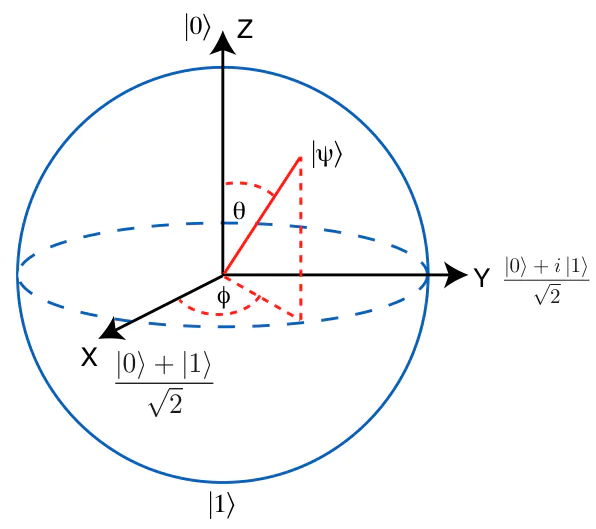
\includegraphics[width=0.6\textwidth]{Immagini troppo complicate/sfera_di_bloch.png}
\end{center}
\caption{\scriptsize La sfera di Bloch}\label{fig:sfera_di_bloch}
\end{figure} 
\noindent Se vogliamo rappresentare un byte, tutto ciò di cui abbiamo bisogno sono otto bit, ovvero otto cifre. Se invece vogliamo rappresentare un qubyte, abbiamo bisogno di un vettore appartenente allo spazio $\mathbb{C}^{2^8} = \mathbb{C}^{256}$. Quindi ci servirebbero 256 numeri complessi per rappresentare un qubyte. Questo aumento esponenziale delle cifre (e quindi della memoria) necessarie per la sola rappresentazione di un registro a più qubit rappresenta uno dei motivi per cui oggi si sta cercando di realizzare computer quantistici. È infatti possibile eseguire computazioni basate su qubit anche su computer classici, di fatto simulando l'esecuzione su computer quantistico, ma questo porta a una perdita esponenziale dell'efficienza.

\subsection{Sovrapposizione}
Abbiamo accennato al fatto che un qubit può trovarsi in molti più stati rispetto a un bit classico. In generale, un qubit $\ket{q}$ si troverà nello stato:
\begin{displaymath}
\ket{q} = 
\begin{bmatrix}
\alpha\\
\beta
\end{bmatrix}
= \alpha \ket{0} + \beta \ket{1}, \; \alpha, \beta \in \mathbb{C}, \; \left\lvert \alpha \right\rvert^{2} + \left\lvert \beta \right\rvert^{2} = 1.
\end{displaymath}
In particolare possiamo dire che l'ampiezza di $\ket{0}$ è $\alpha$, mentre quella di $\ket{1}$ è $\beta$. Quando $\alpha$ è pari a 1, $\beta$ è pari a 0, e il qubit si trova nello stato di base computazionale $\ket{0}$, mentre quando questi valori delle ampiezze si invertono, ovvero quando $\alpha = 0$ e $\beta = 1$, il qubit si trova nello stato di base computazionale $\ket{1}$. Quando sia $\alpha$ che $\beta$ hanno un valore diverso da 0, si dice che il qubit è in uno stato di \emph{sovrapposizione}. Per convenzione, le computazioni quantistiche partono con tutti i qubit nello stato $\ket{0}$, e passando attraverso specifiche porte, che vedremo nella prossima sezione di questo capitolo, possono entrare in uno stato di sovrapposizione. In tutto questo, vi è un vincolo che lo stato di un qubit deve rispettare: \emph{il vettore che lo rappresenta deve essere unitario}, ovvero la sua norma (lunghezza) deve essere pari a uno. In formule, stiamo chiedendo che:
\begin{displaymath}
\left\lVert \ket{q} \right\rVert = \left\lVert
\begin{bmatrix}
\alpha\\
\beta
\end{bmatrix}
\right\rVert
= \sqrt{\left\lvert \alpha \right\rvert^{2} + \left\lvert \beta \right\rvert^{2}} = 1 ,
\end{displaymath}
quindi ci basta verificare che:
\begin{displaymath}
\left\lvert \alpha \right\rvert^{2} + \left\lvert \beta \right\rvert^{2} = 1 .
\end{displaymath}
Il motivo di ciò verrà spiegato nella prossima sezione. È da notare inoltre che quindi gli stati di un qubit sono infiniti, ma non coincidono con gli infiniti vettori dello spazio $\mathbb{C}^{2}$.

\subsection{Misurazione}
In generale, se qualcuno ci fornisce un qubit preparato in uno stato di sovrapposizione, non abbiamo modo di scoprire i valori di $\alpha$ e $\beta$. %E questo è un peccato, dato che, se invece fossimo in grado di leggerli, vorrebbe dire che potremmo conservare informazioni classiche, codificate sotto forma di numeri complessi, all'interno delle ampiezze di un qubit. Possiamo tuttavia ottenere comunque dell'informazione classica partendo da un quantum bit, mediante un processo conosciuto col nome di \emph{misurazione}. 
Ma possiamo comunque ottenere dell'informazione classica da un qubit mediante un processo conosciuto col nome di \emph{misurazione}.
Misurando un qubit possiamo ottenere come risultato solo 0 oppure 1, anche se questo si trova in uno stato di sovrapposizione. In particolare, dato il qubit $\ket{q}$ nello stato:
\begin{displaymath}
\ket{q} = 
\begin{bmatrix}
\alpha\\
\beta
\end{bmatrix}
= \alpha \ket{0} + \beta \ket{1} ,
\end{displaymath}
la probabilità di misurarlo in un bit classico e ottenere come risultato 0 è pari a $\left\lvert \alpha \right\rvert^{2}$, mentre la probabilità di ottenere 1 come risultato della misurazione è pari a $\left\lvert \beta \right\rvert^{2}$. Dato che stiamo parlando di probabilità, la loro somma deve fare 1, ovvero:
\begin{displaymath}
    \left\lvert \alpha \right\rvert^{2} + \left\lvert \beta \right\rvert^{2} = 1,
\end{displaymath}
che è il motivo per cui avevamo richiesto che il vettore rappresentativo di un qubit fosse unitario. Facciamo notare, come ultima cosa, che nella misurazione di un qubit contano non solo le ampiezze, ma anche la base computazionale scelta. Prendiamo per esempio il qubit $\ket{q}$, dove:
\begin{displaymath}
    \ket{q} =
    \begin{bmatrix}
    1\\
    0
    \end{bmatrix} = 
    1 \ket{0} + 0 \ket{1} = 1 
    \begin{bmatrix}
    1\\
    0
    \end{bmatrix} + 0 
    \begin{bmatrix}
    0\\
    1
    \end{bmatrix}.
\end{displaymath}
Se misuriamo questo qubit rispetto alla base Z, sicuramente otteniamo come risultato 0. Lo stesso qubit lo possiamo però esprimere rispetto ai vettori $\ket{+}$ e $\ket{-}$ della base X, ovvero:
\begin{displaymath}
    \ket{q} =
    \begin{bmatrix}
    1\\
    0
    \end{bmatrix} = 
    \frac{1}{\sqrt{2}} \ket{+} + \frac{1}{\sqrt{2}} \ket{-} = 
    \frac{1}{\sqrt{2}} \frac{1}{\sqrt{2}} 
    \begin{bmatrix}
    1\\
    1
    \end{bmatrix} + 
    \frac{1}{\sqrt{2}} \frac{1}{\sqrt{2}} 
    \begin{bmatrix*}[r]
    1\\
    -1
    \end{bmatrix*},
\end{displaymath}
dove $\alpha = \beta = \frac{1}{\sqrt{2}}$. Quindi, se misuriamo il qubit $\ket{q}$ rispetto alla base X, la probabilità di leggere 0 è $\left\lvert \frac{1}{\sqrt{2}} \right\rvert^{2} = \frac{1}{2}$, così come quella di leggere 1. Essendo consapevoli di questo, nel resto del capitolo supporremo che tutte le nostre misurazioni vengano fatte rispetto alla base Z.

\section{Porte quantistiche a singolo qubit}
Un qubit che si trova sempre nello stesso stato non è molto interessante, pertanto ci piacerebbe avere a disposizione degli strumenti per manipolarli. Questi strumenti vengono chiamati \emph{porte}, e sono del tutto analoghe a quelle usate per i bit classici. Normalmente infatti un circuito classico è composto da una serie di bit che cambiano nel tempo attraversando porte NOT, AND, OR, XOR, etc.. Nel caso quantistico la cosa non è tanto diversa: possiamo costruire un circuito quantistico a uno o più qubit, modificando poi questi ultimi con delle porte. Analizzeremo pertanto in questa sezione alcune porte a singolo qubit, per poi concentrarci nella prossima in quelle che coinvolgono due o più qubit contemporaneamente.
\subsection{Porta NOT o X}
La prima porta che esaminiamo è la porta NOT, chiamata anche porta X, che è parzialmente analoga a quella classica. Essa infatti porta un qubit che si trova nello stato $\ket{0}$ nello stato $\ket{1}$ e viceversa. Ma cosa succede ad un qubit che si trova in uno stato di sovrapposizione? Per capirlo, dobbiamo prima esaminare la \emph{rappresentazione matriciale} della porta NOT:
\begin{displaymath}
X =
\begin{bmatrix}
0 & 1\\
1 & 0
\end{bmatrix}.
\end{displaymath}
Ogni porta quantistica infatti può essere rappresentata come una matrice quadrata. In generale, data una porta che accetta in ingresso $n$ qubit, questa avrà dimensione $2^{n} \times 2^{n}$. Nel caso delle porte a singolo qubit quindi abbiamo a che fare con matrici $2 \times 2$. Questa rappresentazione matriciale non dovrebbe stupirci più di tanto: dato che operiamo con dei vettori complessi, è naturale che per manipolarli ci sia bisogno di matrici a coefficienti complessi. Una cosa meno immediata da capire invece è che tutte le matrici che rappresentano porte quantistiche devono essere \emph{unitarie}. Una generica matrice quadrata $U$ si dice unitaria quando:
\begin{displaymath}
U^{\dagger} U = I ,
\end{displaymath}
dove con $I$ intendiamo la matrice identità, %che presenta zeri dappertutto tranne che sulla diagonale principale, popolata da uni, 
mentre con $U^{\dagger}$ intendiamo la matrice trasposta coniugata di $U$. Talvolta $U^{\dagger}$ viene anche chiamata l'\emph{aggiunta} di $U$. Il motivo per cui richiediamo che queste matrici siano unitarie è che, moltiplicandole per un qualunque vettore, la lunghezza di quest'ultimo rimane inalterata, ovvero:
\begin{displaymath}
\left\lVert \ket{\psi} \right\rVert = \left\lVert U \ket{\psi} \right\rVert = 1 ,
\end{displaymath}
dove con $\ket{\psi}$ intendiamo un generico vettore che abbia la stessa dimensione della matrice $U$, che nel nostro caso potrebbe essere un qubit o un registro di questi. Il fatto che un qubit passi attraverso una porta rappresentata da una matrice unitaria è un bene, perché ciò vuol dire che la sua lunghezza (pari a uno) rimane inalterata, e quindi la somma delle ampiezze sotto modulo e al quadrato (ovvero la somma delle probabilità) rimane sempre uno.\\
Fissati questi concetti, possiamo rispondere alla domanda iniziale: come si comporta la porta X quando applicata a un qubit in uno stato di sovrapposizione? Immaginiamo di avere il nostro solito qubit $\ket{q}$ dove le ampiezze sono $\alpha$ e $\beta$. Allora, applicando la porta X, otteniamo:
\begin{displaymath}
X \ket{q} = 
\begin{bmatrix}
0 & 1\\
1 & 0
\end{bmatrix}
\begin{bmatrix}
\alpha\\
\beta
\end{bmatrix} = 
\begin{bmatrix}
\beta\\
\alpha
\end{bmatrix}.
\end{displaymath}
Quindi l'effetto netto è che i valori delle ampiezze si invertono. L'ultima cosa che dobbiamo considerare per completezza è la rappresentazione circuitale della porta X:
\begin{displaymath}
\Qcircuit @C=1em @R=1em {
\lstick{\ket{q}} & \gate{X} \qw & \qw
}
\end{displaymath}
In generale, in un circuito quantistico, rappresenteremo con un quadrato una porta quantistica a singolo qubit, dove la lettera all'interno identifica la particolare porta usata, mentre con una linea orizzontale un semplice cavo, che può essere anche visto come l'applicazione della matrice identità I.

\subsection{Porta R_{x}}
La porta X in realtà è un caso particolare di una porta più generale, la porta $R_{x}$. Abbiamo infatti visto, con la Figura \ref{fig:sfera_di_bloch}, che un qubit può essere visualizzato come un vettore in una sfera unitaria, dove abbiamo anche evidenziato gli assi X, Y e Z. Ebbene, la porta $R_x(\phi)$, che vuole come parametro un angolo, da un punto di vista geometrico non fa altro che prendere il vettore rappresentativo di un qubit e ruotarlo di $\phi$ gradi rispetto all'asse X. La sua rappresentazione matriciale in particolare è:
\begin{displaymath}
    R_x(\phi) = 
    \begin{bmatrix*}[r]
    \cos(\frac{\phi}{2}) & -i\sin(\frac{\phi}{2})\\
    -i\sin(\frac{\phi}{2}) & \cos(\frac{\phi}{2})
    \end{bmatrix*},
\end{displaymath}
dove la porta X corrisponde alla porta $R_x(\phi)$ con $\phi = \pi$. Per esserne sicuri tuttavia svolgiamo un secondo i calcoli:
\begin{displaymath}
    R_x(\pi) = 
    \begin{bmatrix*}[r]
    \cos(\frac{\pi}{2}) & -i\sin(\frac{\pi}{2})\\
    -i\sin(\frac{\pi}{2}) & \cos(\frac{\pi}{2})
    \end{bmatrix*} =
    \begin{bmatrix*}[r]
    0 & -i\\
    -i & 0
    \end{bmatrix*} = -i
    \begin{bmatrix*}[r]
    0 & 1\\
    1 & 0
    \end{bmatrix*} .
\end{displaymath}
Otteniamo dunque che la porta $R_x(\phi)$ è uguale alla porta X, a meno di una costante moltiplicativa $-i$. Potremmo allora concludere che non è vero che le due porte sono uguali, ma saremmo nel torto, perché dobbiamo considerare un altro elemento della computazione quantistica: il \emph{fattore di fase globale}. Con questo termine andiamo ad indicare un numero complesso $e^{i\theta}$ che, se moltiplicato per il vettore rappresentativo di un qualunque qubit, non cambia le nostre probabilità di misura. Più formalmente dovremmo dire che, dato un generico qubit $\ket{\psi}$, il vettore $e^{i\theta}\ket{\psi}$ è equivalente al vettore $\ket{\psi}$ a meno di un fattore di fase globale. Questo vuol dire che la probabilità di misurare 0 nel prima caso è uguale a quella di misurare 0 nel secondo, e lo stesso dicasi per la probabilità di misurare 1. Infatti, applicando la porta X a un qubit $\ket{\psi}$, così come l'abbiamo conosciuta nella Sezione 1.2.1, otterremo il vettore $\ket{\psi}'$, dove:
\begin{displaymath}
    \ket{\psi}' = X \ket{\psi} = 
    \begin{bmatrix}
    0 & 1\\
    1 & 0
    \end{bmatrix}
    \begin{bmatrix}
    \alpha\\
    \beta
    \end{bmatrix} = 
    \begin{bmatrix}
    \beta\\
    \alpha
    \end{bmatrix} ,
\end{displaymath}
mentre applicando la porta $R_x(\pi)$ otterremo il vettore $\ket{\psi}''$, definito come:
\begin{displaymath}
    \ket{\psi}'' = R_x(\pi) \ket{\psi} = -i 
    \begin{bmatrix}
    0 & 1\\
    1 & 0
    \end{bmatrix}
    \begin{bmatrix}
    \alpha\\
    \beta
    \end{bmatrix} = -i 
    \begin{bmatrix}
    \beta\\
    \alpha
    \end{bmatrix} =
    \begin{bmatrix}
    -i \beta\\
    -i \alpha
    \end{bmatrix} .
\end{displaymath}
Ora, definendo $\alpha = a_1 + i a_2$, $\beta = b_1 + i b_2$ e facendo i calcoli, ci rendiamo conto che le probabilità di misura sono le stesse in entrambi i casi:
\begin{displaymath}
\left\lvert \alpha \right\rvert^{2} = \left\lvert a_{1} + i a_{2} \right\rvert^{2} = \left(\sqrt{a_{1}^{2} + a_{2}^2}\right)^{2} = a_{1}^{2} + a_{2}^2\, ,
\end{displaymath}
\begin{displaymath}
\left\lvert -i\alpha \right\rvert^{2} = \left\lvert -i(a_{1} + i a_{2}) \right\rvert^{2} =  \left\lvert -i a_{1} - i^{2} a_{2} \right\rvert^{2} = \left\lvert a_{2} -i a_{1} \right\rvert^{2} = \left(\sqrt{a_{1}^{2} + a_{2}^2}\right)^{2} = a_{1}^{2} + a_{2}^2\, ,
\end{displaymath}

\begin{displaymath}
\left\lvert \beta \right\rvert^{2} = \left\lvert b_{1} + i b_{2} \right\rvert^{2} = \left(\sqrt{b_{1}^{2} + b_{2}^2}\right)^{2} = b_{1}^{2} + b_{2}^2\, ,
\end{displaymath}
\begin{displaymath}
\left\lvert -i\beta \right\rvert^{2} = \left\lvert -i(b_{1} + i b_{2}) \right\rvert^{2} =  \left\lvert -i b_{1} - i^{2} b_{2} \right\rvert^{2} = \left\lvert b_{2} -i b_{1} \right\rvert^{2} = \left(\sqrt{b_{1}^{2} + b_{2}^2}\right)^{2} = b_{1}^{2} + b_{2}^2\, ,
\end{displaymath}
pertanto le due porte provocano lo stesso effetto. In generale applicare un fattore di fase globale a un qubit non cambia i risultati che otterremo dalla computazione, ma esamineremo nel prossimo capitolo, dedicato all'algoritmo di Grover, un caso in cui, all'interno di un sistema a più qubit, questo fattore fa la differenza. Segue la rappresentazione circuitale della porta:
\begin{displaymath}
\Qcircuit @C=1em @R=1em {
\lstick{\ket{q}} & \gate{R_{x}(\phi)} \qw & \qw
}
\end{displaymath}
Come ultima cosa, ci teniamo a mettere in evidenza un aspetto interessante di questa porta. Partendo da un qubit iniziale che si trova nello stato $\ket{0}$ e applicandogli la porta $R_x(\phi)$ con $\phi \neq \pi$ e $\phi \neq 2\pi$, portiamo il nostro qubit in uno stato di sovrapposizione. Talvolta porte $R_x$ come quella appena descritta vengono anche chiamate porte \emph{Partial-NOT}. Proviamo allora ad applicare, a scopo dimostrativo, la porta $R_x(\frac{\pi}{2})$ a un qubit nello stato $\ket{0}$:
\begin{displaymath}
\begin{bmatrix*}[r]
    \cos(\frac{\pi}{4}) & -i\sin(\frac{\pi}{4})\\
    -i\sin(\frac{\pi}{4}) & \cos(\frac{\pi}{4})
\end{bmatrix*}
\begin{bmatrix}
    1\\
    0
\end{bmatrix} = 
\begin{bmatrix*}[r]
    \frac{\sqrt{2}}{2} & -i\frac{\sqrt{2}}{2}\\
    -i\frac{\sqrt{2}}{2} & \frac{\sqrt{2}}{2}
\end{bmatrix*}
\begin{bmatrix}
    1\\
    0
\end{bmatrix} = 
\begin{bmatrix*}[r]
\frac{\sqrt{2}}{2}\\
-i \frac{\sqrt{2}}{2}
\end{bmatrix*} =
\begin{bmatrix*}[r]
\frac{1}{\sqrt{2}}\\
\frac{-i}{\sqrt{2}}
\end{bmatrix*} .
\end{displaymath}
Quello che otteniamo è uno stato di sovrapposizione in cui abbiamo la stessa probabilità di misurare 0 o 1.

\subsection{Porta H}

Un'altra porta molto interessante è la porta H, abbreviazione di porta di \emph{Hadamard}. La sua matrice associata è:
\begin{displaymath}
H = \frac{1}{\sqrt{2}}
\begin{bmatrix*}[r]
1 & 1\\
1 & -1
\end{bmatrix*} .
\end{displaymath}
Se applichiamo questa porta a un qubit che si trova in uno degli stati di base computazionale ($\ket{0}$ o $\ket{1}$), otteniamo una sovrapposizione in cui si ha la stessa probabilità di misurare 0 o 1. Infatti:
\begin{displaymath}
H \ket{0} = \frac{1}{\sqrt{2}}
\begin{bmatrix*}[r]
1 & 1\\
1 & -1
\end{bmatrix*}
\begin{bmatrix}
1\\
0
\end{bmatrix} = 
\begin{bmatrix}
\frac{1}{\sqrt{2}}\\
\frac{1}{\sqrt{2}}
\end{bmatrix} , \; 
H \ket{1} = \frac{1}{\sqrt{2}}
\begin{bmatrix*}[r]
1 & 1\\
1 & -1
\end{bmatrix*}
\begin{bmatrix}
0\\
1
\end{bmatrix} = 
\begin{bmatrix*}[r]
\frac{1}{\sqrt{2}}\\
-\frac{1}{\sqrt{2}}
\end{bmatrix*} .
\end{displaymath}
Notiamo tra l'altro che questi stati di sovrapposizione coincidono con i vettori della base X:
\begin{displaymath}
\ket{+} = \frac{\ket{0} + \ket{1}}{\sqrt{2}} =
\begin{bmatrix}
\frac{1}{\sqrt{2}}\\
\frac{1}{\sqrt{2}}
\end{bmatrix} , \;
\ket{-} = \frac{\ket{0} - \ket{1}}{\sqrt{2}} =
\begin{bmatrix*}[r]
\frac{1}{\sqrt{2}}\\
-\frac{1}{\sqrt{2}}
\end{bmatrix*} .
\end{displaymath}
Infine, la rappresentazione circuitale della porta di Hadamard:
\begin{displaymath}
\Qcircuit @C=1em @R=1em {
\lstick{\ket{q}} & \gate{H} \qw & \qw
}
\end{displaymath}

\subsection{Porte Y e Z}
Abbiamo detto che la porta $R_x$ ci permette di effettuare una rotazione del vettore unitario di un qubit rispetto all'asse X, e che la porta X non è altro che un caso particolare dell'applicazione della porta $R_x$, dove l'angolo di rotazione è pari a $\pi$ radianti. Analogamente a ciò, esistono delle porte che ci permettono di ruotare il vettore rispetto agli assi Y e Z, che non molto sorprendentemente si chiamano $R_y$ e $R_z$. Queste tuttavia non sono particolarmente interessanti per i nostri scopi, quindi non le approfondiremo. Citiamo però per completezza le porte Y e Z, anch'esse casi particolari delle rispettive porte di rotazione con angolo pari a $\pi$ radianti:
\begin{displaymath}
Y = 
\begin{bmatrix*}[r]
0 & -i\\
i & 0
\end{bmatrix*} , \;
Z = 
\begin{bmatrix*}[r]
1 & 0\\
0 & -1
\end{bmatrix*} .
\end{displaymath}
Le matrici X, Y e Z vengono inoltre raggruppate sotto il nome di \emph{matrici di Pauli}.

\section{Porte quantistiche a più qubit}
Così come un bit da solo non ci permette di fare molto, allo stesso modo un singolo qubit, anche se manipolato da diverse porte, non ci condurrà a dei risultati troppo interessanti. In questa sezione pertanto esamineremo alcune porte che manipolano contemporaneamente più qubit alla volta, esaminando anche i concetti di \emph{entanglement} e \emph{uncomputation}.
\subsection{Porta C-NOT}
La prima porta a più qubit che vediamo è forse quella più semplice di tutte: la porta \emph{C-NOT}, abbreviazione di \emph{Controlled-NOT}, che agisce su due qubit alla volta. In particolare, nell'utilizzo di questa porta, si definisce un qubit di controllo e uno target. Quando il qubit di controllo si trova nello stato $\ket{0}$, non succede nulla (di fatto la porta non si attiva). Quando però il suo stato è pari a $\ket{1}$, quello del qubit target si inverte, passando da $\ket{0}$ a $\ket{1}$ e viceversa. Indicando con $\ket{c}$ il qubit di controllo e con $\ket{t}$ quello target, l'effetto complessivo che questa porta applica al sistema a due qubit, che indicheremo con $\ket{ct} = \ket{c} \otimes \ket{t}$, è riassumibile come:
\begin{displaymath}
\ket{00} \rightarrow \ket{00}
\end{displaymath}
\begin{displaymath}
\ket{01} \rightarrow \ket{01}
\end{displaymath}
\begin{displaymath}
\ket{10} \rightarrow \ket{11}
\end{displaymath}
\begin{displaymath} 
\hspace{0.25cm} \ket{11} \rightarrow \ket{10} ,
\end{displaymath}
dove con $\ket{c} \otimes \ket{t}$ intendiamo il prodotto tensore tra due vettori, ovvero:
\begin{displaymath}
\ket{c} \otimes \ket{t} = 
\begin{bmatrix}
c_0\\
c_1
\end{bmatrix} \otimes
\begin{bmatrix}
t_0\\
t_1
\end{bmatrix} = 
\begin{bmatrix}
c_0 t_0\\
c_0 t_1\\
c_1 t_0\\
c_1 t_1
\end{bmatrix} .
\end{displaymath}
La sua forma circuitale invece è:
\begin{displaymath}
\Qcircuit @C=1em @R=1em {
\lstick{\ket{c}} & \ctrl{1} & \rstick{\ket{c}} \qw \\
\lstick{\ket{t}} & \targ & \rstick{\ket{c \oplus t}} \qw
}
\end{displaymath}
Prima di procedere è bene fissare la rappresentazione vettoriale di un sistema a più qubit. Cominciamo da un esempio. In un caso semplice come quello appena descritto, dove abbiamo a che fare con soltanto due qubit, vale la seguente associazione stato-vettore:
\begin{displaymath}
\ket{00} = 
\begin{bmatrix}
1\\
0\\
0\\
0
\end{bmatrix} , \;
\ket{01} = 
\begin{bmatrix}
0\\
1\\
0\\
0
\end{bmatrix} , \;
\ket{10} = 
\begin{bmatrix}
0\\
0\\
1\\
0
\end{bmatrix} , \;
\ket{11} = 
\begin{bmatrix}
0\\
0\\
0\\
1
\end{bmatrix}.
\end{displaymath}
In generale, dato un sistema a $n$ qubit, lo stato di questo sistema verrà rappresentato da un vettore complesso appartenente allo spazio $\mathbb{C}^{2^{n}}$. Inoltre questo vettore è sempre sottoposto al vincolo unitario, ovvero la sua norma deve essere uno, in formule:
\begin{equation}\label{norm_two}
\left\lVert v \right\rVert = \sqrt{\sum_{i=1}^{n}\left\lvert v_{i} \right\rvert^{2}} = 1,
\end{equation}
dove $v$ è un vettore dello spazio $\mathbb{C}^{2^{n}}$. Sapendo questo, possiamo ora mostrare la matrice associata alla porta C-NOT:
\begin{displaymath}
\mbox{C-NOT} = 
\begin{bmatrix}
1 & 0 & 0 & 0\\
0 & 1 & 0 & 0\\
0 & 0 & 0 & 1\\
0 & 0 & 1 & 0
\end{bmatrix} ,
\end{displaymath}
che ci spiega anche cosa succede a un generico stato del nostro sistema a due qubit $\ket{ct} = \alpha \ket{00} + \beta \ket{01} + \gamma \ket{10} + \delta \ket{11}$:
\begin{displaymath}
\begin{bmatrix}
1 & 0 & 0 & 0\\
0 & 1 & 0 & 0\\
0 & 0 & 0 & 1\\
0 & 0 & 1 & 0
\end{bmatrix} 
\begin{bmatrix}
\alpha\\
\beta\\
\gamma\\
\delta
\end{bmatrix} = 
\begin{bmatrix}
\alpha\\
\beta\\
\delta\\
\gamma
\end{bmatrix} .
\end{displaymath}
\subsection{Porta Toffoli}
Una porta che ci piacerebbe portare dall'ambito classico a quello quantistico è la porta AND, che normalmente prende in input due bit e ne restituisce uno che ha come valore 1 solo se i bit di ingresso erano a loro volta nello stato 1. Nel contesto quantistico purtroppo l'eleganza di questa porta non viene mantenuta, ed è necessario usare tre qubit anziché due per svolgere l'operazione di AND. Questo perché ogni circuito quantistico deve mantenere la proprietà di \emph{reversibilità}, che esamineremo più a fondo nella Sezione 1.3.4. In particolare questa porta viene chiamata \emph{porta di Toffoli}, e prende in ingresso tre qubit, che chiameremo $\ket{x}, \ket{y}$ e $\ket{z}$. L'operazione effettuata è quella di AND tra i qubit $\ket{x}$ e $\ket{y}$, ma il risultato viene conservato all'interno del qubit $\ket{z}$. In definitiva, quello che fa questa porta è applicare una porta NOT al qubit $\ket{z}$ quando gli altri due qubit si trovano nello stato $\ket{1}$. La sua forma circuitale forse rende meglio l'idea:
\begin{displaymath}
\Qcircuit @C=1em @R=1em {
\lstick{\ket{x}} & \ctrl{2} & \rstick{\ket{x}} \qw \\
\lstick{\ket{y}} & \ctrl{1} & \rstick{\ket{y}} \qw \\
\lstick{\ket{z}} & \targ & \rstick{\ket{z \oplus (x \land y)}} \qw
}
\end{displaymath}
Come abbiamo però ormai imparato, non c'è porta senza matrice, e quella della porta di Toffoli è:
\begin{displaymath}
\begin{bmatrix}
1 & 0 & 0 & 0 & 0 & 0 & 0 & 0 \\
0 & 1 & 0 & 0 & 0 & 0 & 0 & 0 \\
0 & 0 & 1 & 0 & 0 & 0 & 0 & 0 \\
0 & 0 & 0 & 1 & 0 & 0 & 0 & 0 \\
0 & 0 & 0 & 0 & 1 & 0 & 0 & 0 \\
0 & 0 & 0 & 0 & 0 & 1 & 0 & 0 \\
0 & 0 & 0 & 0 & 0 & 0 & 0 & 1 \\
0 & 0 & 0 & 0 & 0 & 0 & 1 & 0
\end{bmatrix} .
\end{displaymath}
È naturalmente possibile comporre più porte di questo tipo per ottenere una funzione di AND che prende in input un numero arbitrario di argomenti, proprio come nel caso classico. Ne vedremo un esempio nella Sezione 1.3.4.
\subsection{Entanglement}
Fino ad ora ci siamo concentrati su porte quantistiche a più qubit facendole però sembrare una trasposizione uno a uno della loro controparte classica. La loro vera potenza risiede tuttavia negli effetti che queste provocano su sistemi a più qubit quando abbiamo a che fare con stati di sovrapposizione. Può infatti verificarsi un fenomeno singolare tra di essi, che Einstein aveva chiamato ``\emph{spooky action at a distance}'': i qubit possono entrare in \emph{entanglement} tra loro. Ciò vuol dire che i qubit coinvolti in questo fenomeno condividono in qualche modo lo stesso ``destino'', ovvero un'azione compiuta su uno di essi avrà ripercussioni anche sugli altri, indipendentemente dalla distanza che li separa. Possiamo avere un'idea di cosa questo significhi dando uno sguardo a una porta costruibile a partire da due già viste: la \emph{porta C-NOT parziale}. Essa è ottenibile dalla composizione di una porta $R_x$ con una \textit{C-NOT}:
\begin{displaymath}
\Qcircuit @C=1em @R=1em {
\lstick{\ket{x}} & \gate{R_x(\phi)} & \ctrl{1} & \qw \\
\lstick{\ket{y}} & \qw              & \targ    & \qw
}
\end{displaymath}
Prima di studiarne gli effetti dobbiamo però capire che cosa succede quando applichiamo una porta a singolo qubit in un circuito multi-qubit. Abbiamo detto che il cavo quantistico può essere visto come un'applicazione della matrice identità $I$ a un qubit. Pertanto in questo caso stiamo applicando parallelamente una porta $R_x$ al primo qubit, e una $I$ al secondo. La matrice associata a questa trasformazione è ottenuta effettuando il prodotto di Kronecker, conosciuto anche come prodotto tensore, tra le matrici relative alle due porte coinvolte. In generale date due matrici $A$ e $B$ di dimensione qualsiasi, il loro prodotto tensore è definito come:
\begin{displaymath}
A \otimes B = 
\begin{bmatrix}
a_{11} B & a_{12} B & \dots  & a_{1m} B\\
a_{21} B & a_{22} B & \dots  & a_{2m} B\\
\vdots   & \vdots   & \ddots & \vdots\\
a_{n1} B & a_{n2} B & \dots  & a_{nm} B\\
\end{bmatrix} .
\end{displaymath}
Fissando a titolo dimostrativo l'angolo $\phi$ a $\frac{\pi}{2}$ radianti, pertanto, il prodotto tensore tra le matrici associate alle porte $R_x(\frac{\pi}{2})$ e $I$ risulta:
\begin{displaymath}
R_x\left(\frac{\pi}{2}\right) \otimes I = 
\begin{bmatrix*}[r]
\frac{\sqrt{2}}{2} I & -i \frac{\sqrt{2}}{2} I\\
-i \frac{\sqrt{2}}{2} I & \frac{\sqrt{2}}{2} I
\end{bmatrix*} =
\begin{bmatrix*}[r]
\frac{\sqrt{2}}{2} & 0 & -i \frac{\sqrt{2}}{2} & 0\\
0 & \frac{\sqrt{2}}{2} & 0 & -i \frac{\sqrt{2}}{2}\\
-i \frac{\sqrt{2}}{2} & 0 & \frac{\sqrt{2}}{2} & 0\\
0 & -i \frac{\sqrt{2}}{2} & 0 & \frac{\sqrt{2}}{2}\\
\end{bmatrix*} .
\end{displaymath}
Immaginando che entrambi i qubit $\ket{x}$ e $\ket{y}$ partano dallo stato $\ket{0}$, il vettore associato a questo sistema che otteniamo dopo l'applicazione della prima porta risulta:
\begin{displaymath}
\left( R_x\left(\frac{\pi}{2}\right) \otimes I \right) \ket{00} = 
\begin{bmatrix*}[r]
\frac{\sqrt{2}}{2} & 0 & -i \frac{\sqrt{2}}{2} & 0\\
0 & \frac{\sqrt{2}}{2} & 0 & -i \frac{\sqrt{2}}{2}\\
-i \frac{\sqrt{2}}{2} & 0 & \frac{\sqrt{2}}{2} & 0\\
0 & -i \frac{\sqrt{2}}{2} & 0 & \frac{\sqrt{2}}{2}\\
\end{bmatrix*}
\begin{bmatrix}
1\\
0\\
0\\
0
\end{bmatrix} = 
\begin{bmatrix*}[r]
\frac{\sqrt{2}}{2}\\
0\\
-i \frac{\sqrt{2}}{2}\\
0
\end{bmatrix*} = 
\begin{bmatrix*}[r]
\frac{1}{\sqrt{2}}\\
0\\
\frac{-i}{\sqrt{2}}\\
0
\end{bmatrix*} .
\end{displaymath}
Applichiamo ora la porta C-NOT e vediamo come cambia il vettore:
\begin{displaymath}
\begin{bmatrix}
1 & 0 & 0 & 0\\
0 & 1 & 0 & 0\\
0 & 0 & 0 & 1\\
0 & 0 & 1 & 0
\end{bmatrix}
\begin{bmatrix*}[r]
\frac{1}{\sqrt{2}}\\
0\\
\frac{-i}{\sqrt{2}}\\
0
\end{bmatrix*} = 
\begin{bmatrix*}[r]
\frac{1}{\sqrt{2}}\\
0\\
0\\
\frac{-i}{\sqrt{2}}
\end{bmatrix*} = \frac{1}{\sqrt{2}} \ket{00} - \frac{i}{\sqrt{2}} \ket{11} .
\end{displaymath}
Uno stato del genere dimostra che cosa intendevamo poco fa, quando abbiamo asserito che dei qubit posti in entanglement sono soggetti allo stesso ``destino''. In questo caso infatti abbiamo pari probabilità di misurare o 0 o 1 per entrambi i qubit, ma non capiterà mai che uno venga misurato 0 e l'altro 1 (almeno in caso di assenza di rumore, ma questo è un argomento che tratteremo nella Sezione 1.4.2). Questo era solo uno dei tanti modi con cui dei qubit possono essere posti in entanglement, e ci sono circuiti capaci di legare un numero arbitrario di qubit in questo modo.

\subsection{Uncomputation}
Un altro aspetto interessante e per alcuni algoritmi quantistici fondamentale è quello dell'\emph{uncomputation}. Per capirlo supponiamo di voler costruire un circuito che calcoli l'AND tra tre qubit $\ket{x_1}$, $\ket{x_2}$ e $\ket{x_3}$. Possiamo usare due volte la porta di Toffoli per raggiungere lo scopo:
\begin{displaymath}
\Qcircuit @C=1em @R=1em {
\lstick{\ket{x_1}} & \ctrl{3} & \qw       & \rstick{\ket{x_1}} \qw \\
\lstick{\ket{x_2}} & \ctrl{2} & \qw       & \rstick{\ket{x_2}} \qw \\
\lstick{\ket{x_3}} & \qw       & \ctrl{2} & \rstick{\ket{x_3}} \qw \\
\lstick{\ket{0}}   & \targ     & \ctrl{1} & \rstick{\ket{x_1 \land x_2}} \qw \\
\lstick{\ket{0}}   & \qw       & \targ    & \rstick{\ket{x_1 \land x_2 \land x_3}} \qw\\
}
\end{displaymath}
Effettivamente il quinto qubit del circuito ci dà il risultato desiderato. Tuttavia abbiamo anche accumulato un risultato intermedio nel quarto qubit, ovvero l'AND tra i primi due, che non ci interessa. Ciò potrebbe sembrare un problema di poco conto, ma per algoritmi complessi in cui i qubit vengono posti in entanglement, avere risultati intermedi lasciati in giro può rappresentare un problema. Inoltre il qubit usato per conservare questo AND intermedio potrebbe essere usato per altri scopi se venisse ``resettato'', ovvero riportato nello stato $\ket{0}$. È qui che entra in gioco l'uncomputation, che prevede, una volta calcolato il risultato cercato, di applicare le stesse porte usate per effettuare tale calcolo (ad eccezione di quella che modifica il qubit risultato) nell'ordine inverso, così da riportare i qubit di lavoro, a volta chiamati anche \emph{ancilla qubit} (nel nostro esempio il quarto qubit ricade in questa categoria), nel loro stato originale. Il circuito mostrato sopra verrebbe pertanto modificato come segue:
\begin{displaymath}
\Qcircuit @C=1em @R=1em {
\lstick{\ket{x_1}} & \ctrl{3}  & \qw       & \ctrl{3} & \rstick{\ket{x_1}} \qw \\
\lstick{\ket{x_2}} & \ctrl{2}  & \qw       & \ctrl{2} & \rstick{\ket{x_2}} \qw \\
\lstick{\ket{x_3}} & \qw       & \ctrl{2}  & \qw      & \rstick{\ket{x_3}} \qw \\
\lstick{\ket{0}}   & \targ     & \ctrl{1}  & \targ    & \rstick{\ket{0}} \qw \\
\lstick{\ket{0}}   & \qw       & \targ     &  \qw     & \rstick{\ket{x_1 \land x_2 \land x_3}} \qw\\
}
\end{displaymath}

\section{I qubit odierni}
\subsection{Sistemi fisici per la rappresentazione di qubit}
Fino ad ora abbiamo parlato dei qubit come oggetti puramente matematici, ma fintanto che questi rimangono oggetti astratti, nella pratica, non servono a molto, se non a capirne il funzionamento. Fisicamente, quindi, come viene implementato un qubit? In vari modi. Alcuni di questi possono essere:
\begin{itemize}
    \item un elettrone in due differenti orbitali attorno al nucleo di un atomo.
    \item un fotone in uno tra due stati di polarizzazione.
    \item una particella subatomica che ha una tra le due direzioni di spin.
\end{itemize}
Ad oggi tuttavia è raro trovare implementazioni di qubit soddisfacenti, o almeno tali da permetterci di svolgere calcoli complessi. Perfino implementare un semplice cavo quantistico può essere difficile. Se ad esempio scegliamo di conservare un qubit in un neutrino, allora sarà facile preservare il suo stato nel tempo, dato che i neutrini interagiscono debolmente con il mondo esterno. Tuttavia, se questo è vero, allora sarà difficile manipolare il loro stato con delle porte. L'argomento è complesso e non rientra nei nostri scopi. Ciò che invece riteniamo interessante sottolineare è che ad oggi molti di questi sistemi non sono in grado di compiere calcoli per periodi di tempo troppo lunghi. Questo è dovuto a un problema conosciuto col nome di \emph{rumore}.
\subsection{Rumore nei computer quantistici}
Il rumore è purtroppo un fenomeno che si verifica con costanza nei moderni device quantistici e che va a incidere negativamente sui risultati nelle nostre computazioni. Le sorgenti di rumore possono essere di vario tipo, come i segnali elettromagnetici emessi dalle reti Wi-Fi o perfino disturbi creati dal campo magnetico terrestre. L'effetto netto del rumore è di degradare la qualità dell'informazione che decidiamo di conservare in un sistema di qubit. Può perfino accadere, a causa del rumore, che un qubit inizializzato nello stato $\ket{0}$ e fatto passare attraverso due porte $H$ in sequenza (operazione che coincide con l'applicazione di nessuna porta, dato che $H^{\dagger}H=HH=I$) dia come risultato della misurazione 1, cosa che in un computer quantistico perfetto non potrebbe mai accadere. Infatti le simulazioni svolte su dispositivi classici, che simulano un device quantistico perfetto, non sono soggette a questo fenomeno, ma sono anche molto più lente rispetto alle corrispettive computazioni eseguite su macchine quantistiche. Oggigiorno infatti lo scopo è quello di riuscire a eseguire circuiti quantistici per periodi di tempo sempre più lunghi prima che il rumore corrompa i risultati della computazione. 



\begin{comment}
\begin{displaymath}
\Qcircuit @C=1em @R=1em {
\lstick{\ket{c}} & \ctrl{1} & \rstick{\ket{x}} \qw \\
\lstick{\ket{t}} & \targ & \rstick{\ket{y}} \qw
}
\end{displaymath}
\end{comment}


\chapter{L'algoritmo di Grover}

Nel calcolo classico, se dobbiamo cercare uno specifico oggetto all'interno di un insieme non strutturato che ne contiene $N$, siamo costretti ad esaminare uno a uno gli elementi dell'insieme e controllare se l'elemento corrente è quello cercato. In caso affermativo, la ricerca si interrompe, in caso negativo, la ricerca continua. Questo se diamo per scontato che gli elementi dell'insieme non seguano alcun tipo di ordinamento, altrimenti è possibile usare un algoritmo di ricerca binaria per ridurre la complessità della ricerca a $\mathcal{O}(\log_2 N)$. In caso di assenza di qualsivoglia ordinamento, l'unica cosa che possiamo fare è procedere per esclusione, con una complessità $\mathcal{O}(N)$. Con l'algoritmo di ricerca quantistico, conosciuto anche come \emph{algoritmo di Grover}, è possibile tuttavia ridurre la complessità della ricerca di un fattore quadratico, avendo quindi una complessità $\mathcal{O}(\sqrt{N})$.
Il capitolo è strutturato come segue:
\begin{enumerate}
    \item Nella prima sezione tratteremo del primo elemento che compone l'algoritmo di Grover: l'\emph{oracolo}, cercando di darne un'intuizione.
    \item Nella seconda sezione andremo ad illustrare la procedura per intero.
    \item Nella terza sezione cercheremo di capire la matematica che sta dietro a questa procedura, dando un'interpretazione geometrica ai passi dell'algoritmo così da ``convincerci'' che funzioni.
\end{enumerate}
Durante la lettura delle fonti che trattavano l'argomento, ci siamo resi conto che venivano date per scontate alcune nozioni di geometria e di algebra lineare. Ciò a volte può rallentare l'apprendimento, data la complessità del tema. Onde evitare che ciò accada anche ai lettori di questo testo, ci soffermeremo su alcuni punti che riteniamo meritevoli di maggiore approfondimento. Chi ritenesse di avere sufficiente confidenza con queste nozioni può saltare tranquillamente le parti ad esse dedicate.
\section{L'oracolo}
\subsection{Differenza tra conoscere una soluzione e saper riconoscere una soluzione}
Supponiamo che ci venga fornita una formula 3-SAT come quella della Figura \ref{fig:3_sat_example}, ovvero una formula booleana in forma normale congiuntiva dove tutte le clausole contengono esattamente tre simboli proposizionali.
\begin{figure}[!htb]
\captionsetup{font=scriptsize}
\begin{displaymath}
(A \lor B \lor \lnot C) \land (\lnot A \lor D \lor C) \land (\lnot B \lor \lnot D \lor \lnot A) \land (\lnot C \lor \lnot B \lor D).
\end{displaymath}
\caption{\scriptsize Esempio di formula 3-SAT con 4 simboli proposizionali.}\label{fig:3_sat_example}
\end{figure}\\
Un algoritmo che risolve questo problema è un algoritmo che prova tutte le $2^4$ possibili interpretazioni per la formula, fino a quando non trova un suo modello. Quindi l'algoritmo \emph{non conosce a priori} la soluzione del problema, ma quando ne vede una \emph{sa riconoscerla}. Facciamo un esempio molto alla mano: immaginiamo che il problema di soddisfare la formula booleana della Figura \ref{fig:3_sat_example} faccia parte di un compito d'esame di Logica Per la Programmazione. Ci sono solo due studenti che partecipano alla prova. Il primo non ha studiato, ma la sera prima si è intrufolato nell'ufficio del Professore e ha fatto una copia della soluzione dell'esame, che è riuscito a portarsi in aula senza farsi scoprire. In questo caso, lo studente conosce \emph{a priori} la soluzione del problema, e sta di fatto barando. Per sua sfortuna viene scoperto dal Docente, che gli ritira il testo d'esame e lo boccia sul posto. Il secondo studente invece, %si è preparato per mesi all'esame,
che ha seguito tutte le lezioni studiando in maniera costante, alla fine consegna la sua soluzione, che è in particolare $A=F, B=T, C=T, D=T $. Il Professore, per potergli assegnare un voto, deve \emph{verificare} che la soluzione proposta sia effettivamente una soluzione al problema. Valuta quindi la formula proposizionale nell'interpretazione proposta:
\begin{figure}[!htb]
\captionsetup{font=scriptsize}
\begin{displaymath}
(F \lor T \lor F) \land (T \lor T \lor T) \land (F \lor F \lor T) \land (F \lor F \lor T) \equiv T \land T \land T \land T \equiv T.
\end{displaymath}
\caption{\scriptsize Valutazione della formula nell'interpretazione dello studente.}\label{fig:3_sat_correction}
\end{figure}\\
La soluzione è corretta, e lo studente passa con 30L. Il Docente ha potuto appurare la correttezza della soluzione perché sapeva \emph{riconoscere} un suo modello quando ne vedeva uno. Quando ci si approccia per la prima volta all'algoritmo di Grover, può sembrare che l'oracolo sia in grado di riconoscere la soluzione del problema perché già la conosce: non è così! Sa riconoscere la soluzione perché sa quali vincoli deve rispettare. Da questo punto di vista, l'oracolo sarebbe il nostro Professore dell'esempio, e \textbf{non} lo studente disonesto.

\subsection{Costruire un oracolo}

Torniamo al nostro esempio generale. Vogliamo cercare una soluzione per un problema all'interno di uno spazio di ricerca contenente $N$ elementi. Dato che non sempre è possibile convertire in modo semplice questi oggetti in sequenze binarie (riesce facile se stiamo parlando di interi, ma diventa più difficile se parliamo di oggetti complessi del mondo reale come animali, cose, persone etc..), definiamo una funzione bigettiva $g(x)$ che associa un elemento $x$ dell'insieme ad un \emph{indice} codificato in binario. Per fare ciò ci servono, nel calcolo classico, $n$ bit, dove $N = 2^n$. Stiamo supponendo che $N$ sia una potenza di due per semplificare la spiegazione, ma questa ipotesi non è necessaria. Infatti, qualora $2^n$ fosse maggiore di $N$, assoceremo i $2^n - N$ indici che vanno da $N$ a $2^n$ a un valore fittizio, e sapremo che non potranno mai essere indici di una soluzione. Nel calcolo quantistico l'unica differenza è che invece di $n$ bit avremo $n$ qubit. Così come per la formula 3-SAT della Figura \ref{fig:3_sat_example} non è detto che ci sia un solo modello, allo stesso modo in un problema non è detto che la soluzione sia soltanto una. Indicheremo pertanto con la lettera $M$ il numero di soluzioni all'interno dello spazio di ricerca, dove $0 \leq M \leq N$. Abbiamo bisogno di un ultimo ingrediente per poter costruire il nostro oracolo: una funzione $f(x)$ che restituisce 1 quando $x$ è una soluzione del problema, 0 altrimenti. Più in generale, dovremmo dire che $f(x)$ restituisce 1 quando $x$ è \emph{indice} di una soluzione del problema e 0 altrimenti, ma per semplificare la spiegazione supporremo che la funzione $g(x)$ sia la funzione identità, ovvero che gli indici delle possibili soluzioni rappresentino le possibili soluzioni stesse.
Con queste premesse, l'oracolo può essere visto come una scatola nera (\emph{black box}) che, dati come input un registro degli indici $\ket{x}$, ovvero un registro quantistico a $n$ qubit, e un ulteriore qubit $\ket{q}$, svolge la seguente operazione:

\begin{displaymath}
\ket{x} \ket{q} \xrightarrow{O} \ket{x} \ket{q \oplus f(x)} ,
\end{displaymath}
dove $\oplus$ indica la somma modulo 2. L'operazione ha come obiettivo quello di applicare una porta $NOT$ al qubit $\ket{q}$ quando $\ket{x}$ è una soluzione del problema. Viene infatti sfruttato in questo passo dell'algoritmo un effetto quantistico molto importante: il \emph{kickback di fase}. Per capire al meglio la potenza di questo effetto, facciamo un esempio con 2 qubit.
\clearpage
\begin{ex}
Si consideri il seguente circuito quantistico:
\begin{figure}[!htb]
\captionsetup{font=scriptsize}
\begin{displaymath}
\Qcircuit @C=1em @R=1em {
\lstick{\ket{x}} & \ctrl{1} & \rstick{\ket{x}} \qw \\
\lstick{\ket{y}} & \targ & \rstick{\ket{y}} \qw
}
\end{displaymath}
\caption{\scriptsize Circuito quantistico con una porta \emph{C-NOT}.}\label{fig:cnot-gate}
\end{figure}\\
Si tratta di un semplice circuito dove viene usata una sola porta, la \emph{C-NOT}, che abbiamo visto nella Sezione 1.3.1. %Tale porta ha un qubit \emph{di controllo}, in questo caso $\ket{x}$, e un qubit \emph{obiettivo}, $\ket{y}$. Il simbolo $\oplus$ indica il qubit obiettivo, mentre il pallino più piccolo indica quello di controllo. Tale circuito è da considerarsi come l'implementazione di un semplicissimo programma del tipo:
Algoritmicamente il suo funzionamento può essere espresso da un programma del tipo:
\begin{algorithm}[H]
\begin{algorithmic}[1]
    \If{$x = 1$} 
        \Let{$y$}{$1 \oplus y$}
    \Else
        \State{do nothing}
    \EndIf
\end{algorithmic}
\end{algorithm}
\noindent Come però abbiamo già studiato, l'effetto della porta \emph{C-NOT} è ben più generale di così, e consiste nell'applicare, a un generico circuito a due qubit del tipo $\ket{xy} = \alpha \ket{00} + \beta \ket{01} + \gamma \ket{10} + \delta \ket{11}$, la seguente trasformazione lineare:
%Sostanzialmente inverte il valore del qubit obiettivo quando quello di controllo ha come valore $\ket{1}$. Questa definizione ha senso fintanto che i due qubit possono assumere come valori i due stati di base computazionale $\ket{0}$ e $\ket{1}$. Ma il bello dei qubit è proprio che possono assumere valori più complessi (o meglio, \emph{più valori contemporaneamente}) e entrare in \emph{entaglement} tra loro. Più in generale, dati i qubit $\ket{x} = \alpha \ket{0} + \beta \ket{1}$ e $\ket{y} = \gamma \ket{0} + \delta \ket{1}$, la porta $CNOT$ applica la seguente trasformazione lineare:
 
\begin{displaymath}
\begin{bmatrix}
1 & 0 & 0 & 0\\
0 & 1 & 0 & 0\\
0 & 0 & 0 & 1\\
0 & 0 & 1 & 0
\end{bmatrix}
\begin{bmatrix}
\alpha \\
\beta \\
\gamma \\
\delta
\end{bmatrix}
=
\begin{bmatrix}
\alpha \\
\beta \\
\delta \\
\gamma
\end{bmatrix}.
\end{displaymath}
Alla luce di questo fatto, vediamo ora un caso particolare. Dal codice sopra e dalla sua implementazione quantistica potrebbe sembrare che il qubit di controllo rimanga sempre inalterato, e faccia semplicemente da discriminante per il valore del secondo qubit. Tuttavia considerando due qubit negli stati computazionali $\ket{+}$ e $\ket{-}$, ottenuti applicando una porta di Hadamard a due qubit rispettivamente nello stato di base computazionale $\ket{0}$ e $\ket{1}$, osserviamo un effetto interessante, mostrato nella Figura \ref{fig:cnot-gate-incredible}:
\begin{figure}[!htb]
\captionsetup{font=scriptsize}
\begin{displaymath}
\Qcircuit @C=1em @R=1em {
\lstick{\ket{+}} & \ctrl{1} & \rstick{\ket{-}} \qw \\
\lstick{\ket{-}} & \targ & \rstick{\ket{-}} \qw
}
\end{displaymath}
\caption{\scriptsize Circuito con porta \emph{C-NOT} dove il qubit di controllo cambia, mentre quello obiettivo rimane inalterato.}\label{fig:cnot-gate-incredible}
\end{figure}\\
Dato che il circuito da solo non rende bene l'idea, eseguiamo i calcoli a mano per convincerci che funziona:
\begin{displaymath}
\ket{+-} = \frac{\ket{0}+\ket{1}}{\sqrt{2}} \otimes \frac{\ket{0}-\ket{1}}{\sqrt{2}} = \frac{\ket{00}}{2} - \frac{\ket{01}}{2} + \frac{\ket{10}}{2} - \frac{\ket{11}}{2} = 
\begin{bmatrix*}[r]
\frac{1}{2} \\
-\frac{1}{2} \\
\frac{1}{2} \\
-\frac{1}{2}
\end{bmatrix*} ,
\end{displaymath}

\begin{displaymath}
\begin{bmatrix}
1 & 0 & 0 & 0\\
0 & 1 & 0 & 0\\
0 & 0 & 0 & 1\\
0 & 0 & 1 & 0
\end{bmatrix}
\begin{bmatrix*}[r]
\frac{1}{2} \\
-\frac{1}{2} \\
\frac{1}{2} \\
-\frac{1}{2}
\end{bmatrix*}
=
\begin{bmatrix*}[r]
\frac{1}{2} \\
-\frac{1}{2} \\
-\frac{1}{2} \\
\frac{1}{2}
\end{bmatrix*},
\end{displaymath}

\begin{displaymath}
\ket{--} = \frac{\ket{0}-\ket{1}}{\sqrt{2}} \otimes \frac{\ket{0}-\ket{1}}{\sqrt{2}} = \frac{\ket{00}}{2} - \frac{\ket{01}}{2} - \frac{\ket{10}}{2} + \frac{\ket{11}}{2} = 
\begin{bmatrix*}[r]
\frac{1}{2} \\
-\frac{1}{2} \\
-\frac{1}{2} \\
\frac{1}{2}
\end{bmatrix*}.
\end{displaymath}
Abbiamo quindi trovato un esempio di circuito a più qubit dove \emph{il qubit di controllo viene modificato da quello obiettivo}. Questo fenomeno è conosciuto come kickback di fase.
\end{ex}
I motivi per cui vogliamo applicare questo particolare effetto al qubit $\ket{q}$ dell'oracolo saranno chiari quando daremo un'interpretazione geometrica dell'algoritmo. Per il momento però è bene sottolineare un'ultima volta un concetto importante: \emph{l'oracolo non conosce la soluzione a priori, ma è in grado di riconoscerne una quando la vede}. Riteniamo questo punto fondamentale in quanto l'oracolo è un pezzo importantissimo dell'algoritmo di Grover, eppure spesso viene liquidato dicendo che è una scatola nera capace di riconoscere la soluzione, ma non viene mai fatto vedere \emph{come} fa a riconoscerla. Apriamo quindi questa scatola nera e vediamo come potrebbe essere implementato l'oracolo relativo al problema della Figura \ref{fig:3_sat_example}, mediante un circuito quantistico. Per fare ciò tuttavia dobbiamo prima modificare la formula applicando la regola di De Morgan per il calcolo proposizionale. Supponiamo inoltre che ogni qubit sia inizializzato nello stato di base computazionale $\ket{0}$:
\begin{figure}[!htb]
\captionsetup{font=scriptsize}

\begin{flalign*}
&(A \lor B \lor \lnot C) \land (\lnot A \lor D \lor C) \land (\lnot B \lor \lnot D \lor \lnot A) \land (\lnot C \lor \lnot B \lor D) \\
&\equiv \mkern50mu \{(De Morgan)\} \\
&(\lnot A \land \lnot B \land C) \land (A \land \lnot D \land \lnot C) \land (B \land D \land A) \land (C \land B \land \lnot D).
\end{flalign*}

\begin{displaymath}
\Qcircuit @C=1em @R=1em {
\lstick{\ket{A}} & \ctrlo{4} & \ctrl{5}  & \ctrl{6} & \qw       & \qw       & \qw       & \ctrl{6}  & \ctrl{5}  & \ctrlo{4} & \qw \\
\lstick{\ket{B}} & \ctrlo{3} & \qw       & \ctrl{5} & \ctrl{6}  & \qw       & \ctrl{6}  & \ctrl{5}  & \qw       & \ctrlo{3} & \qw \\
\lstick{\ket{C}} & \ctrl{2}  & \ctrlo{3} & \qw      & \ctrl{5}  & \qw       & \ctrl{5}  & \qw       & \ctrlo{3} & \ctrl{2}  & \qw \\
\lstick{\ket{D}} & \qw       & \ctrlo{2} & \ctrl{3} & \ctrlo{4} & \qw       & \ctrlo{4} & \ctrl{3}  & \ctrlo{2} & \qw       & \qw \\
\lstick{\ket{0}} & \targ     & \qw       & \qw      & \qw       & \ctrlo{4} & \qw       & \qw       & \qw       & \targ     & \qw \\
\lstick{\ket{0}} & \qw       & \targ     & \qw      & \qw       & \ctrlo{3} & \qw       & \qw       & \targ     & \qw       & \qw \\
\lstick{\ket{0}} & \qw       & \qw       & \targ    & \qw       & \ctrlo{2} & \qw       & \targ     & \qw       & \qw       & \qw \\
\lstick{\ket{0}} & \qw       & \qw       & \qw      & \targ     & \ctrlo{1} & \targ     & \qw       & \qw       & \qw       & \qw \\
\lstick{\ket{q}} & \gate{X}  & \gate{H}  & \qw      & \qw       & \targ     & \qw       & \qw       & \qw       & \qw       & \qw
}
\end{displaymath}
\caption{\scriptsize Oracolo relativo al problema 3-SAT della figura \ref{fig:3_sat_example}, capace di riconoscerne una soluzione.}\label{fig:oracle_1}
\end{figure}\\
I primi quattro qubit rappresentano i simboli proposizionali, dove $\ket{0} = F$ e $\ket{1} = T$, mentre i quattro successivi sono qubit di lavoro (\emph{ancilla qubit}), utili solo a conservare i risultati intermedi della computazione. L'ultimo qubit invece è quello che applicherà il kickback di fase qualora $\ket{ABCD}$ rappresentasse un'interpretazione che soddisfa la formula logica. Il pallino bianco nelle porte di Toffoli indica, come quello nero, un qubit di controllo, con la differenza che richiede il valore $\ket{0}$ per attivarsi. Il motivo per cui $\ket{q}$ viene inizializzato nello stato $\ket{-}$, mediante l'applicazione delle porte $X$ e $H$ in sequenza, è che così facendo è possibile applicare il kickback di fase sui primi quattro qubit, lasciando inalterato l'ultimo. Si noti inoltre che si è sfruttato il meccanismo della \emph{uncomputation} per ripristinare lo stato dei qubit ancilla. L'effetto complessivo dell'oracolo può quindi essere riassunto come:
\begin{displaymath}
\ket{x} \ket{-} \xrightarrow{O} (-1)^{f(x)} \ket{x} \ket{-},
\end{displaymath}
poiché i qubit di lavoro tornano al loro stato originale grazie alla \emph{uncomputation} e il qubit $q$ rimane sempre nello stato $\ket{-}$, applicando eventualmente un kickback di fase -1 al registro quantistico quando questo contiene una soluzione al problema. Nel nostro esempio, $\ket{x} = \ket{ABCD}$.

\section{L'iterazione di Grover}
L'algoritmo di per sé non è troppo complicato, e richiede veramente poche componenti. La prima cosa da fare è, dato un registro quantistico a $n$ qubit nello stato $\ket{0}^{\otimes n}$, far passare tale registro attraverso una porta $H^{\otimes{n}}$. Detto in altre parole, si comincia avendo tutti gli $n$ qubit nello stato di base computazionale $\ket{0}$, per poi far passare ciascuno di essi attraverso una porta di Hadamard così da porre in entaglement i qubit e ottenere lo \emph{stato di ugual sovrapposizione} $\ket{\psi}$, dove:
\begin{displaymath}
\ket{\psi} = \frac{1}{\sqrt{N}}\sum_{x=0}^{N-1}\ket{x}.
\end{displaymath}
Ricordiamo che $N=2^{n}$, dove $N$ è la dimensione del dominio di ricerca e $n$ è il numero di qubit che usiamo per rappresentare gli indici degli oggetti in tal dominio.
\begin{ex}
Con 3 qubit, lo stato di ugual sovrapposizione sarebbe:
\begin{displaymath}
\ket{\psi} = \frac{1}{\sqrt{8}}\ket{000} + \frac{1}{\sqrt{8}}\ket{001} + \frac{1}{\sqrt{8}}\ket{010} + \frac{1}{\sqrt{8}}\ket{011} + \frac{1}{\sqrt{8}}\ket{100} + \frac{1}{\sqrt{8}}\ket{101} + \frac{1}{\sqrt{8}}\ket{110} + \frac{1}{\sqrt{8}}\ket{111} .
\end{displaymath}
\end{ex}
Dopo questa inizializzazione l'algoritmo di Grover si riduce ad un'applicazione reiterata di una funzione quantistica (funzione intesa come subroutine informatica) chiamata \emph{iterazione di Grover} o \emph{operatore di Grover}, che denotiamo con la lettera $G$. Questa procedura può essere divisa in quattro passi:
\begin{enumerate}
    \item Si applica l'oracolo $O$.
    \item Si applica la trasformazione di Hadamard $H^{\otimes n}$ al registro quantistico a $n$ qubit.
    \item Si applica un kickback di fase -1 ad ogni stato di base computazionale del registro eccetto che allo stato $\ket{0}$ (ovvero $\ket{0_1 0_2 \dots 0_n}$). Una porta di questo tipo applica la trasformazione lineare $2\ket{0} \bra{0} - I$ al vettore degli stati, che corrisponde a una riflessione attorno al vettore $\ket{0}$.
    \item si applica di nuovo la trasformazioni di Hadamard $H^{\otimes n}$.
\end{enumerate}
Ma quante volte va ripetuta quest'operazione? Al più $\sqrt{N}$ volte, per trovare una soluzione.

\begin{figure}[h!]
\captionsetup{font=scriptsize}
\begin{center}
    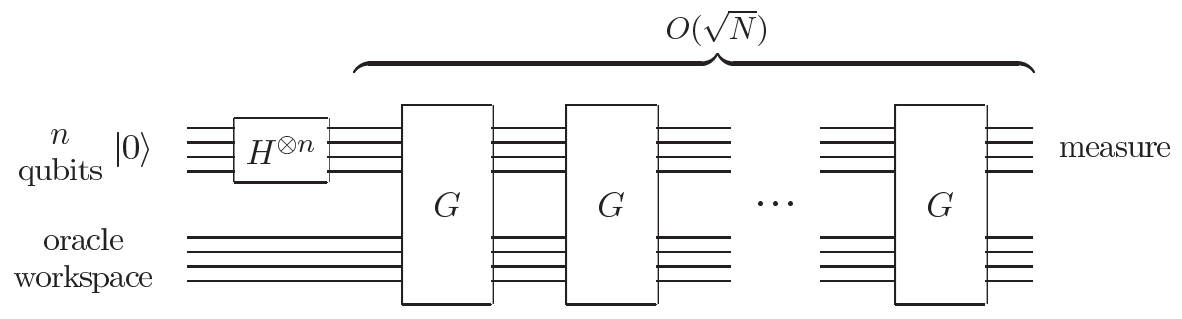
\includegraphics[width=1\textwidth]{img_grover_0.png}
\end{center}
\caption{\scriptsize Rappresentazione schematica dell'algoritmo di ricerca quantistico. Anche se questi impiega dei qubit di lavoro, l'analisi della complessità coinvolge solo il registro a n qubit (si veda il Capitolo 6.1 di \cite{nielsen_chuang})}\label{fig:img_grover_0}
\end{figure} 
\begin{figure}[h!]
\captionsetup{font=scriptsize}
\begin{center}
    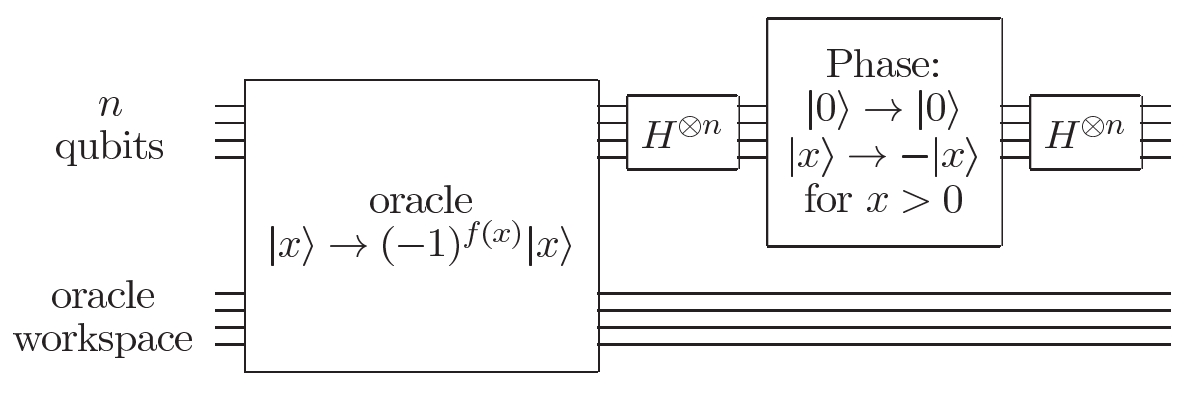
\includegraphics[width=0.80\textwidth]{img_grover_1.png}
\end{center}
\caption{\scriptsize Circuito rappresentativo dell'iterazione di Grover G (si veda Capitolo 6.1 di \cite{nielsen_chuang})}\label{fig:img_grover_1}
\end{figure}
\noindent Quando parliamo di algoritmi non possiamo esimerci dal parlare della loro complessità, e quelli quantistici non fanno eccezione. I passi 2 e 4, ovvero le trasformazioni di Hadamard, hanno un costo lineare nel numero di qubit di $n = \log{(N)}$. Il passo 3 invece può essere implementato con $\mathcal{O}(N)$ porte. Tutta la complessità dell'algoritmo ricade dunque sull'oracolo e sul numero di volte che va invocato, in quanto gli altri passi rimangono identici e costanti indipendentemente dalla formulazione del problema di ricerca. L'implementazione dell'oracolo cambia da problema a problema, come abbiamo visto nella Figura \ref{fig:oracle_1}, pertanto il suo costo, in linea di principio, può essere arbitrariamente alto. Tuttavia per costruirlo solitamente si parte da un circuito classico e lo si converte in forma quantistica, implementando una funzione $f:\{0, 1\}^{n} \rightarrow \{0, 1\}$.
Dato che si tratta di una copia uno a uno di un circuito, non abbiamo modo di controllare la complessità di una singola esecuzione dell'oracolo, che potremmo migliorare solo cercando un algoritmo (e quindi un circuito) classico più efficiente da cui partire.
La vera differenza risiede dunque nel numero di applicazioni dell'oracolo: $\mathcal{O}(N)$ volte in ambito classico, $\mathcal{O}(\sqrt{N})$ in quello quantistico. Quando daremo un'interpretazione geometrica all'algoritmo nella prossima sezione sarà chiaro questo miglioramento quadratico. Per il momento ci accontentiamo di una osservazione finale. I passi 2, 3 e 4 possono essere combinati per ottenere la trasformazione lineare:
\begin{displaymath}
H^{\otimes n} (2\ket{0} \bra{0} - I) H^{\otimes n} = 2\ket{\psi}\bra{\psi} - I,
\end{displaymath}
dove $\ket{\psi}$ è lo stato di ugual sovrapposizione. Un'iterazione di Grover $G$ può quindi essere espressa come l'applicazione del seguente operatore unitario:
\begin{displaymath}
G = (2\ket{\psi}\bra{\psi} - I)O,
\end{displaymath}
dove $O$ è l'operatore oracolo.

\section{Analisi dell'algoritmo}

Per convincersi della correttezza dell'algoritmo di Grover non è possibile esimersi da una sua visualizzazione geometrica. Ciò che faremo in questa sezione sarà pertanto affiancare alla spiegazione testuale degli esempi, procedendo su due binari paralleli ma inseparabili:
\begin{itemize}
    \item Da un lato, useremo un sistema a due qubit per mostrare algebricamente lo svolgimento dell'iterazione di Grover. Il problema giocattolo che prenderemo in considerazione sarà più che banale: dato uno spazio di ricerca contenente i numeri che vanno a 0 a 3 (estremi inclusi), vogliamo che l'algoritmo ci restituisca come soluzione il numero 3, corrispondente allo stato computazionale $\ket{11}$. L'incredibile semplicità e, se vogliamo, stupidità di questo problema ci permetterà di effettuare calcoli chiari e semplici, senza tirare in ballo matrici e vettori troppo grandi.
    \item Dall'altro, per dare un'interpretazione geometrica a questi passi algebrici, mostreremo l'effetto che tali operazioni avrebbero su uno spazio tridimensionale. Notate che questa associazione è puramente a scopo illustrativo: non esiste un numero di qubit capace di formare uno spazio vettoriale in $\mathbb{C}^3$.
    Forse ciò sarebbe possibile se potessimo manipolare un registro quantistico a $\log_2$(3) qubit. \emph{Peccato però che non esista un simile registro, in quanto non avrebbe senso}. Il motivo per cui non abbiamo optato per una rappresentazione geometrica usando 2 qubit è che non è possibile rappresentare efficientemente %uno spazio quadri-dimensionale in uno bidimensionale. 
    lo spazio $\mathbb{C}^4$ su due dimensioni. Allo stesso tempo, non abbiamo usato un sistema a un solo qubit sia per la parte algebrica che per quella geometrica poiché non avrebbe permesso di visualizzare in maniera incisiva il funzionamento dell'algoritmo. Anzi, avremmo rischiato di porre in contrasto tra loro spiegazione scritta e interpretazione geometrica: \emph{un disastro insomma}.
\end{itemize}
L'algoritmo di Grover può essere visualizzato come una rotazione del vettore iniziale $\ket{\psi}$ su un certo piano. Per definire tale piano ci occorrono due ultimi ingredienti. Sappiamo già che $N$ è la dimensione dello spazio di ricerca, mentre $M$ è il numero di soluzioni al problema, dove $0 \leq M \leq N$. Sappiamo anche che $\ket{\psi}$ è il vettore che rappresenta lo stato di ugual sovrapposizione $\frac{1}{\sqrt{N}} \sum_{x=0}^{N-1}\ket{x}$. Definiamo adesso con $\sum^{'}_{x}$ la sommatoria dei vettori $\ket{x}$ che rappresentano una soluzione al problema, e con $\sum^{''}_{x}$ la sommatoria dei vettori $\ket{x}$ che NON sono soluzione del problema. Definiamo dunque due nuovi vettori $\ket{\alpha}$ e $\ket{\beta}$ come segue:
\begin{displaymath}
\ket{\alpha} = \frac{1}{\sqrt{N-M}}\sum_{x}\mathop{}^{''}\ket{x},
\end{displaymath}
\begin{displaymath}
\ket{\beta} = \frac{1}{\sqrt{M}}\sum_{x}\mathop{}^{'}\ket{x}.
\end{displaymath}
Notate che tutti questi vettori sono sempre unitari, ovvero $\left\lVert \ket{\psi} \right\rVert = \left\lVert \ket{\alpha} \right\rVert = \left\lVert \ket{\beta} \right\rVert = 1$, dove, ricordiamo, con $\left\lVert . \right\rVert$ indichiamo la norma unitaria o norma 2 di un vettore, calcolabile mediante la formula:% corrispondente alla sua lunghezza euclidea. Per calcolare la norma di un qualsiasi vettore $v$ in $\mathbb{C}^{n}$ è necessario prendere tutte le sue componenti, farne il modulo, elevarle a quadrato, sommarle e infine prendere la radice quadrata del risultato, in formule:
%\begin{figure}[!htb]
%\captionsetup{font=scriptsize}

\begin{equation}\label{norm_two}
\left\lVert v \right\rVert = \sqrt{\sum_{i=1}^{n}\left\lvert v_{i} \right\rvert^{2}} \, .
\end{equation}

%\caption{\scriptsize Formula per il calcolo della norma di un vettore.}\label{fig:norm_2_formula}
%\end{figure}

\begin{ex}
(Algebra) Nello spazio vettoriale $\mathbb{C}^{4}$ abbiamo:
\begin{displaymath}
\ket{\psi} = \frac{1}{\sqrt{4}}\sum_{x=0}^{3}\ket{x} = \frac{1}{\sqrt{4}}\ket{00} + \frac{1}{\sqrt{4}}\ket{01} + \frac{1}{\sqrt{4}}\ket{10} + \frac{1}{\sqrt{4}}\ket{11} = \frac{1}{\sqrt{4}} \begin{bmatrix}
1 \\
1 \\
1 \\
1 
\end{bmatrix},
\end{displaymath}
dove, ricordiamo, stiamo cercando come soluzione 3, ovvero vorremmo misurare lo stato di base computazionale $\ket{11}$. Quindi $N=4$ e $M=1$. Non semplificheremo $\sqrt{4}$ con 2 in quanto vogliamo che sia sempre chiaro che quel $\sqrt{4}$ è un'istanza di $\sqrt{N}$. Inoltre:
\begin{displaymath}
\sum_{x}\mathop{}^{'}\ket{x} = \begin{bmatrix}
0 \\
0 \\
0 \\
1
\end{bmatrix},
\mkern50mu \sum_{x}\mathop{}^{''}\ket{x} = \begin{bmatrix}
1 \\
1 \\
1 \\
0
\end{bmatrix},
\end{displaymath}
\begin{displaymath}
\ket{\beta} = \frac{1}{\sqrt{1}}\sum_{x}\mathop{}^{'}\ket{x} = \begin{bmatrix}
0 \\
0 \\
0 \\
1
\end{bmatrix}, \mkern50mu \ket{\alpha} = \frac{1}{\sqrt{3}}\sum_{x}\mathop{}^{''}\ket{x} = \frac{1}{\sqrt{3}} \begin{bmatrix}
1 \\
1 \\
1 \\
0
\end{bmatrix}.
\end{displaymath}
(Geometria) Immaginiamo di avere, nello spazio vettoriale $\mathbb{R}^{3}$:
\begin{displaymath}
\ket{\psi} = \frac{1}{\sqrt{3}} \begin{bmatrix}
1 \\
1 \\
1
\end{bmatrix},
\end{displaymath}
dove definiamo le due sommatorie e i vettori $\ket{\alpha}$ e $\ket{\beta}$ come:
\begin{displaymath}
\sum_{x}\mathop{}^{'}\ket{x} = \begin{bmatrix}
0 \\
0 \\
1
\end{bmatrix},
\mkern50mu \sum_{x}\mathop{}^{''}\ket{x} = \begin{bmatrix}
1 \\
1 \\
0
\end{bmatrix},
\end{displaymath}
\begin{displaymath}
\ket{\beta} = \frac{1}{\sqrt{1}}\sum_{x}\mathop{}^{'}\ket{x} = \begin{bmatrix}
0 \\
0 \\
1
\end{bmatrix}, \mkern50mu \ket{\alpha} = \frac{1}{\sqrt{2}}\sum_{x}\mathop{}^{''}\ket{x} = \frac{1}{\sqrt{2}} \begin{bmatrix}
1 \\
1 \\
0
\end{bmatrix}.
\end{displaymath}
Nello spazio tridimensionale ci troviamo dunque nella situazione della figura \ref{fig:3d_figure_1}:

\begin{figure}[H]
\captionsetup{font=scriptsize}
\centering
\begin{tikzpicture}[x=3cm, y=3cm, z=-1.8cm]
    % Axes
    \draw [->] (0,0,0) -- (1,0,0) node [right] {$y$};
    \draw [->] (0,0,0) -- (0,1,0) node [right] {$z$};
    \draw [->] (0,0,0) -- (0,0,1) node [left] {$x$};
    % Vectors
    \draw [->, thick] (0,0,0) -- (0.5773502692, 0.5773502692, 0.5773502692);
    \draw [->, thick] (0,0,0) -- (0,1,0);
    \draw [->, thick] (0,0,0) -- (0.7071067812, 0, 0.7071067812);
  
    % Dashed lines
    \draw [loosely dashed]
        (0, 0, 0.5773502692) -- (0.5773502692, 0, 0.5773502692) -- (0.5773502692, 0, 0)
        (0.5773502692, 0, 0.5773502692) -- (0.5773502692, 0.5773502692, 0.5773502692)
        (0, 0, 0.5773502692) -- (0, 0.5773502692, 0.5773502692) -- (0, 0.5773502692, 0)
        (0, 0.5773502692, 0.5773502692) -- (0.5773502692, 0.5773502692, 0.5773502692)
        (0.5773502692, 0, 0) -- (0.5773502692, 0.5773502692, 0) -- (0, 0.5773502692, 0)
        (0.5773502692, 0.5773502692, 0) -- (0.5773502692, 0.5773502692, 0.5773502692)
        
        (0.7071067812, 0, 0) -- (0.7071067812, 0, 0.7071067812) -- (0, 0, 0.7071067812)
        
        ;
    % Labels
     \node [left] at (0,1,0) {$\ket{\beta}$};
     \node [right] at (0.5773502692, 0.5773502692, 0.5773502692) {$\ket{\psi}$};
     \node [right] at (0.7071067812, 0, 0.7071067812) {$\ket{\alpha}$};
     

\end{tikzpicture}
\caption{\scriptsize Rappresentazione di $\ket{\alpha}$, $\ket{\beta}$ e $\ket{\psi}$ nello spazio $\mathbb{R}^3$.}\label{fig:3d_figure_1}
\end{figure}

\end{ex}
Prima di procedere, notiamo una cosa che può darci un'intuizione circa la natura dei vettori $\ket{\alpha}$ e $\ket{\beta}$. Questi vettori, così come tutti i vettori che possiamo trovare in ambito quantistico, sono unitari, ovvero hanno lunghezza uno. Ciò è in linea con il fatto che la somma delle probabilità deve fare uno. 
Infatti sappiamo dal Capitolo 1 che nella misurazione di un qubit (o di un sistema a più qubit posti in entanglement tra loro) la probabilità di misurare un certo stato corrisponde all'ampiezza di quello stato in valore assoluto e elevata alla seconda. La somma di queste probabilità è proprio l'Equazione~\eqref{norm_two}, a meno della radice quadrata. Ma dato che $\sqrt{1} = 1$, la radice ce la possiamo anche scordare. I vettori $\ket{\alpha}$ e $\ket{\beta}$ in particolare hanno, per ogni loro componente con un'ampiezza diversa da 0, la stessa ampiezza: $\frac{1}{\sqrt{K}}$, dove $K$ è uguale proprio al numero di componenti diverse da 0. Solo che:
\begin{itemize}
    \item $\ket{\alpha}$ ha come uniche componenti diverse da 0 quelle che NON rappresentano una soluzione al problema. Ciò vuol dire che non importa quante volte misuriamo questo vettore, otterremo sempre un fallimento per il problema. Potremmo anche chiamarlo, vista la equidistribuzione di probabilità, \emph{vettore di ugual sovrapposizione dei fallimenti}. Per $\ket{\alpha}$, abbiamo $K$ = $N-M$, poiché $N-M$ sono i fallimenti (totale - successi).
    \item $\ket{\beta}$ è esattamente l'opposto: ha come uniche componenti diverse da 0 quelle che rappresentano una soluzione al problema, così che ogni sua misura ci restituisca un successo per il problema. Di nuovo, queste componenti hanno la stessa ampiezza, pertanto possiamo chiamarlo anche \emph{vettore di ugual sovrapposizione dei successi}. Per $\ket{\beta}$, $K$ = $M$, poiché $M$ sono le soluzioni.
\end{itemize}
È quindi come se $\ket{\alpha}$ prendesse tutti e soli i fallimenti di $\ket{\psi}$ distribuendo le ampiezze equamente, e lo stesso facesse $\ket{\beta}$, ma con le soluzioni. Questa intuizione trova un corrispettivo algebrico nel fatto che $\ket{\psi}$ appartiene allo span di $\ket{\alpha}$ e $\ket{\beta}$. Infatti:
\begin{displaymath}
\ket{\psi} = \sqrt{\frac{N-M}{N}} \ket{\alpha} \mkern5mu + \mkern5mu \sqrt{\frac{M}{N}} \ket{\beta} = \sqrt{\frac{N-M}{N}} \frac{1}{\sqrt{N-M}} \sum_{x}\mathop{}^{''}\ket{x} \mkern5mu + \mkern5mu \sqrt{\frac{M}{N}} \frac{1}{\sqrt{M}}\sum_{x}\mathop{}^{'}\ket{x} = 
\end{displaymath}
\begin{displaymath}
= \frac{1}{\sqrt{N}} ( \sum_{x}\mathop{}^{''}\ket{x} +  \sum_{x}\mathop{}^{'}\ket{x} ) = \ket{\psi}.
\end{displaymath}
Le rotazioni che l'algoritmo di Grover esegue in successione servono, algebricamente, ad ``allargare'' le ampiezze delle soluzioni e ``schiacciare'' quelle degli insuccessi, e geometricamente ad avvicinare il più possibile il vettore iniziale $\ket{\psi}$ al vettore di \emph{soluzione assicurata} $\ket{\beta}$, idealmente sovrapponendo il primo al secondo. \\
Possiamo compiere una rotazione effettuando due riflessioni in successione: la prima volta rispetto a $\ket{\alpha}$, la seconda rispetto a $\ket{\psi}$. Dato che usare lo stesso termine per due concetti diversi può portare confusione, indicheremo d'ora in poi con $\ket{\phi}$ il vettore che vogliamo ruotare prima rispetto a $\ket{\alpha}$ e poi rispetto a $\ket{\psi}$ per avvicinarlo il più possibile a $\ket{\beta}$. Notate che questo vettore all'inizio coincide con $\ket{\psi}$, ma ciò non vale più dopo la prima iterazione di Grover. %Diventa chiaro dopo aver eseguito la prima rotazione.
Se indichiamo con $\frac{\theta}{2}$ l'angolo compreso tra $\ket{\psi}$ e $\ket{\alpha}$, ogni rotazione ci permette di avvicinarci di $\theta$ radianti al vettore di ugual sovrapposizione dei successi. Vediamo come. Innanzitutto, riflettiamo il vettore $\ket{\phi}$ rispetto a $\ket{\alpha}$. Dato che stiamo parlando di vettori unitari farlo è molto semplice, basta applicare l'operatore di riflessione $2\ket{\alpha}\bra{\alpha}-I$ al vettore che vogliamo ruotare, $\ket{\phi}$. Chiamando $\ket{\phi'}$ il vettore risultante, otteniamo:
\begin{displaymath}
(2\ket{\alpha}\bra{\alpha}-I) \ket{\phi} = \ket{\phi'}.
\end{displaymath}

\begin{ex}
(Algebra) L'operatore di riflessione rispetto al vettore $\ket{\alpha}$ risulta:
\begin{displaymath}
2\ket{\alpha}\bra{\alpha} - I = 2 \frac{1}{\sqrt{3}}\begin{bmatrix}
1 \\
1 \\
1 \\
0
\end{bmatrix}
\frac{1}{\sqrt{3}} \begin{bmatrix}
1 & 1 & 1 & 0 \\
\end{bmatrix}
- I = \frac{2}{3} \begin{bmatrix}
1 & 1 & 1 & 0 \\
1 & 1 & 1 & 0 \\
1 & 1 & 1 & 0 \\
0 & 0 & 0 & 0 
\end{bmatrix}
- \begin{bmatrix}
1 & 0 & 0 & 0 \\
0 & 1 & 0 & 0 \\
0 & 0 & 1 & 0 \\
0 & 0 & 0 & 1 \\
\end{bmatrix} = \begin{bmatrix*}[r]
-\frac{1}{3} & \frac{2}{3} & \frac{2}{3} & 0 \\
\frac{2}{3} & -\frac{1}{3} & \frac{2}{3} & 0 \\
\frac{2}{3} & \frac{2}{3} & -\frac{1}{3} & 0 \\
0 & 0 & 0 & -1
\end{bmatrix*}.
\end{displaymath}
Otteniamo pertanto:
\begin{displaymath}
\ket{\phi'} = (2\ket{\alpha}\bra{\alpha}-I) \ket{\phi} = \begin{bmatrix*}[r]
-\frac{1}{3} & \frac{2}{3} & \frac{2}{3} & 0 \\
\frac{2}{3} & -\frac{1}{3} & \frac{2}{3} & 0 \\
\frac{2}{3} & \frac{2}{3} & -\frac{1}{3} & 0 \\
0 & 0 & 0 & -1
\end{bmatrix*}
\frac{1}{\sqrt{4}}
\begin{bmatrix}
1 \\
1 \\
1 \\
1
\end{bmatrix}
= 
\frac{1}{\sqrt{4}} \begin{bmatrix*}[r]
1 \\
1 \\
1 \\
-1
\end{bmatrix*}.
\end{displaymath}
(Geometria) In questo caso l'operatore di riflessione risulta:
\begin{displaymath}
2\ket{\alpha}\bra{\alpha} - I = 2 \frac{1}{\sqrt{2}}\begin{bmatrix}
1 \\
1 \\
0
\end{bmatrix}
\frac{1}{\sqrt{2}} \begin{bmatrix}
1 & 1 & 0 \\
\end{bmatrix}
- I = \frac{2}{2} \begin{bmatrix}
1 & 1 & 0 \\
1 & 1 & 0 \\
0 & 0 & 0 \\
\end{bmatrix}
- \begin{bmatrix}
1 & 0 & 0 \\
0 & 1 & 0 \\
0 & 0 & 1 
\end{bmatrix} = \begin{bmatrix*}[r]
0 & 1 & 0 \\
1 & 0 & 0 \\
0 & 0 & -1
\end{bmatrix*}.
\end{displaymath}
Dunque:
\begin{displaymath}
\ket{\phi'} = (2\ket{\alpha}\bra{\alpha}-I) \ket{\phi} = \begin{bmatrix*}[r]
0 & 1 & 0 \\
1 & 0 & 0 \\
0 & 0 & -1
\end{bmatrix*}
\frac{1}{\sqrt{3}}
\begin{bmatrix}
1 \\
1 \\
1 
\end{bmatrix}
= 
\frac{1}{\sqrt{3}} \begin{bmatrix*}[r]
1 \\
1 \\
-1
\end{bmatrix*}.
\end{displaymath}
Abbiamo così ruotato $\ket{\phi}$ attorno a $\ket{\alpha}$, che tridimensionalmente corrisponde alla seguente situazione:
\begin{figure}[H]
\captionsetup{font=scriptsize}

\centering
\begin{tikzpicture}[x=3cm, y=3cm, z=-1.8cm]
    % Axes
    \draw [->] (0,0,0) -- (1,0,0) node [right] {$y$};
    \draw [->] (0,0,0) -- (0,1,0) node [right] {$z$};
    \draw [->] (0,0,0) -- (0,0,1) node [left] {$x$};
    % Vectors
    %psi, beta e alpha
    \draw [->, thick] (0,0,0) -- (0.5773502692, 0.5773502692, 0.5773502692);
    \draw [->, thick] (0,0,0) -- (0,1,0);
    \draw [->, thick] (0,0,0) -- (0.7071067812, 0, 0.7071067812);
    %phi'
    \draw [->, thick] (0,0,0) -- (0.5773502692, -0.5773502692, 0.5773502692);
  
    % Dashed lines
    \draw [loosely dashed]
        %psi
        %(0, 0, 0.5773502692) -- (0.5773502692, 0, 0.5773502692) -- (0.5773502692, 0, 0)
        %(0.5773502692, 0, 0.5773502692) -- (0.5773502692, 0.5773502692, 0.5773502692)
        %(0, 0, 0.5773502692) -- (0, 0.5773502692, 0.5773502692) -- (0, 0.5773502692, 0)
        %(0, 0.5773502692, 0.5773502692) -- (0.5773502692, 0.5773502692, 0.5773502692)
        %(0.5773502692, 0, 0) -- (0.5773502692, 0.5773502692, 0) -- (0, 0.5773502692, 0)
        %(0.5773502692, 0.5773502692, 0) -- (0.5773502692, 0.5773502692, 0.5773502692)
        
        %alpha
        (0.7071067812, 0, 0) -- (0.7071067812, 0, 0.7071067812) -- (0, 0, 0.7071067812)
        
        ;
    % Labels
     \node [left] at (0,1,0) {$\ket{\beta}$};
     \node [right] at (0.5773502692, 0.5773502692, 0.5773502692) {$\ket{\psi}$};
     \node [right] at (0.7071067812, 0, 0.7071067812) {$\ket{\alpha}$};
     \node [right] at (0.5773502692, -0.5773502692, 0.5773502692) {$\ket{\phi'}$};

\end{tikzpicture}
\caption{\scriptsize Rotazione del vettore $\ket{\phi}$ nello spazio $\mathbb{R}^3$. Notare che, 
anche se può non sembrare a causa del fatto che stiamo rappresentando uno spazio tridimensionale in uno bidimensionale, anche il vettore $\ket{\phi'}$ è normalizzato, proprio come gli altri. Infatti in questa prima rotazione si ha che $\ket{\psi} = \ket{\phi} = [\phi_1, \phi_2, \phi_3]$, e $\ket{\phi'} = [\phi_1, \phi_2, -\phi_3]$.}\label{fig:3d_figure_2}
\end{figure}
\end{ex}
%Dato che l'angolo tra $\ket{\psi}$ e $\ket{\alpha}$ era di $\frac{\theta}{2}$ radianti, a seguito di questa rotazione abbiamo ottenuto un vettore $\ket{\phi'}$ distante $\theta$ radianti da $\ket{\psi}$.
Il prossimo passo è compiere la seconda riflessione, stavolta rispetto al vettore di ugual sovrapposizione $\ket{\psi}$.
%Questo ci avvicinerà di $\theta$ radianti a $\ket{\beta}$.
Di nuovo, possiamo usare l'operatore di riflessione $2\ket{\psi}\bra{\psi}-I$, così da ruotare il vettore $\ket{\phi'}$ e ottenere il vettore $\ket{\phi''}$, ovvero:
\begin{displaymath}
(2\ket{\psi}\bra{\psi}-I) \ket{\phi'} = \ket{\phi''}.
\end{displaymath}
\begin{ex}
(Algebra) L'operatore di riflessione rispetto al vettore $\ket{\psi}$ risulta:
\begin{displaymath}
2\ket{\psi}\bra{\psi} - I = 2 \frac{1}{\sqrt{4}}\begin{bmatrix}
1 \\
1 \\
1 \\
1
\end{bmatrix}
\frac{1}{\sqrt{4}} \begin{bmatrix}
1 & 1 & 1 & 1 \\
\end{bmatrix}
- I = \frac{2}{4} \begin{bmatrix}
1 & 1 & 1 & 1 \\
1 & 1 & 1 & 1 \\
1 & 1 & 1 & 1 \\
1 & 1 & 1 & 1 
\end{bmatrix}
- \begin{bmatrix}
1 & 0 & 0 & 0 \\
0 & 1 & 0 & 0 \\
0 & 0 & 1 & 0 \\
0 & 0 & 0 & 1 \\
\end{bmatrix} = \begin{bmatrix*}[r]
-\frac{1}{2} & \frac{1}{2} & \frac{1}{2} & \frac{1}{2} \\
\frac{1}{2} & -\frac{1}{2} & \frac{1}{2} & \frac{1}{2} \\
\frac{1}{2} & \frac{1}{2} & -\frac{1}{2} & \frac{1}{2} \\
\frac{1}{2} & \frac{1}{2} & \frac{1}{2} & -\frac{1}{2} \\
\end{bmatrix*}.
\end{displaymath}
Pertanto:
\begin{displaymath}
\ket{\phi''} = (2\ket{\alpha}\bra{\alpha}-I) \ket{\phi'} = 
\begin{bmatrix*}[r]
-\frac{1}{2} & \frac{1}{2} & \frac{1}{2} & \frac{1}{2} \\
\frac{1}{2} & -\frac{1}{2} & \frac{1}{2} & \frac{1}{2} \\
\frac{1}{2} & \frac{1}{2} & -\frac{1}{2} & \frac{1}{2} \\
\frac{1}{2} & \frac{1}{2} & \frac{1}{2} & -\frac{1}{2} \\
\end{bmatrix*}
\frac{1}{\sqrt{4}} \begin{bmatrix*}[r]
1 \\
1 \\
1 \\
-1
\end{bmatrix*}
= 
\begin{bmatrix}
0 \\
0 \\
0 \\
1
\end{bmatrix},
\end{displaymath}
che in questo caso corrisponde proprio al vettore $\ket{\beta}$. Ci è bastata quindi una sola rotazione per ottenere proprio il risultato che volevamo. Occhio però che questo avviene perché siamo in un sistema a due qubit con una soluzione, in generale ci vogliono più rotazioni, e non sempre si finisce esattamente su $\ket{\beta}$, ma ci si arriva molto vicino. \\
(Geometria) L'operatore di riflessione rispetto a $\ket{\psi}$ risulta:
\begin{displaymath}
2\ket{\psi}\bra{\psi} - I = 2 \frac{1}{\sqrt{3}}\begin{bmatrix}
1 \\
1 \\
1
\end{bmatrix}
\frac{1}{\sqrt{3}} \begin{bmatrix}
1 & 1 & 1 \\
\end{bmatrix}
- I = \frac{2}{3} \begin{bmatrix}
1 & 1 & 1 \\
1 & 1 & 1 \\
1 & 1 & 1 \\
\end{bmatrix}
- \begin{bmatrix}
1 & 0 & 0 \\
0 & 1 & 0 \\
0 & 0 & 1 
\end{bmatrix} = \begin{bmatrix*}[r]
-\frac{1}{3} & \frac{2}{3} & \frac{2}{3}\\
\frac{2}{3} & -\frac{1}{3} & \frac{2}{3}\\
\frac{2}{3} & \frac{2}{3} & -\frac{1}{3}
\end{bmatrix*}.
\end{displaymath}
Così otteniamo:
\begin{displaymath}
\ket{\phi''} = (2\ket{\psi}\bra{\psi}-I) \ket{\phi'} = \begin{bmatrix*}[r]
-\frac{1}{3} & \frac{2}{3} & \frac{2}{3}\\
\frac{2}{3} & -\frac{1}{3} & \frac{2}{3}\\
\frac{2}{3} & \frac{2}{3} & -\frac{1}{3}
\end{bmatrix*}
\frac{1}{\sqrt{3}}
\begin{bmatrix*}[r]
1 \\
1 \\
-1 
\end{bmatrix*}
= 
\frac{1}{\sqrt{3}} \begin{bmatrix*}[r]
-\frac{1}{3} \\
-\frac{1}{3} \\
\frac{5}{3}
\end{bmatrix*}.
\end{displaymath}
Geometricamente:
%FUNZIONA! TODO: Ricrea tutte le immagini tikz in documenti standalone, esportale, importale in questo progetto e usale, così la compilazione è più veloce. TIKZ YEAH
\begin{figure}[H]
\begin{center}
\captionsetup{font=scriptsize}
    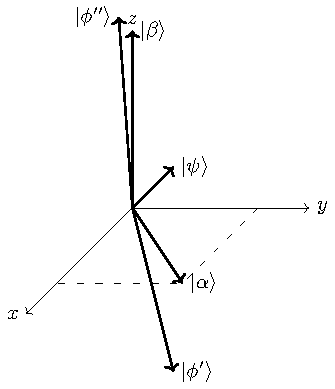
\includegraphics[width=0.32\textwidth]{Immagini troppo complicate/immagine1.pdf}
\caption{\scriptsize Rotazione del vettore $\ket{\phi'}$ rispetto a $\ket{\psi}$. Anche in questo caso il vettore rimane normalizzato, anche se può non sembrare.}\label{fig:3d_figure_3}
\end{center} %TODO: ingrandire se possibile
\end{figure}
\noindent Notate che in questo caso, anche se ci siamo avvicinati alla soluzione, \emph{l'abbiamo addirittura superata}! Come già detto questo esempio geometrico serve solo a visualizzare l'effetto della rotazione e non corrisponde a uno scenario reale, ma ci mette in guardia dal fatto che se ruotiamo indiscriminatamente potremmo anche superare la soluzione. 
\end{ex}
Abbiamo così compiuto la prima rotazione, avvicinandoci di $\theta$ radianti al vettore $\ket{\beta}$. Per capire il perché ragioniamo sugli angoli tra i vettori. L'angolo che separa $\ket{\phi}$ da $\ket{\alpha}$ è di $\frac{\theta}{2}$ radianti. Riflettendo il primo vettore rispetto al secondo, ci siamo allontanati da $\ket{\psi}$ di $\theta$ radianti, ottenendo $\ket{\phi'}$. Infine, riflettendo quest'ultimo rispetto a $\ket{\psi}$, abbiamo ottenuto $\ket{\phi''}$, che è sempre distante $\theta$ radianti da $\ket{\psi}$, ma ``dalla parte opposta''. L'angolo complessivo tra $\ket{\phi''}$ e $\ket{\alpha}$ è quindi di $\frac{3}{2} \theta$ radianti.
Nelle successive iterazioni di Grover il ragionamento rimane lo stesso, solo che il vettore $\ket{\phi''}$ della $i$-esima rotazione diventa il vettore $\ket{\phi}$ della $(i+1)$-esima. Per questo abbiamo distinto il vettore $\ket{\phi}$ dal vettore $\ket{\psi}$: alla prima iterazione corrispondono, ma dalla seconda in poi differiscono. Ma quante volte dobbiamo ruotare per arrivare alla soluzione? Per capirlo, proviamo a vedere il problema da un altro punto di vista.\\
Sia dato un piano cartesiano con una circonferenza di raggio 1 (unitaria) e di centro 0, chiamata anche \emph{circonferenza goniometrica}, come quella della Figura \ref{fig:unitary_circumference}. Costruiamo un triangolo rettangolo su di essa, con ipotenusa il segmento $\overline{OP}$ e cateti le proiezioni di questo sui due assi. Dato l'angolo $\frac{\theta}{2}$ compreso tra l'asse delle ascisse e l'ipotenusa del triangolo, si definisce con sin($\frac{\theta}{2}$) il rapporto tra il cateto opposto all'angolo e l'ipotenusa, e con cos($\frac{\theta}{2}$) il rapporto tra il cateto adiacente e l'ipotenusa (ad essere precisi, il rapporto tra le lunghezze).
\begin{figure}[h!]
\captionsetup{font=scriptsize}
\begin{center}
    \includegraphics[width=0.35\textwidth]{Immagini troppo complicate/immagine1.1.pdf}
\end{center}
\caption{\scriptsize Circonferenza unitaria avente $\overline{OP}$ come ipotenusa e x e y come cateti.}\label{fig:unitary_circumference}
\end{figure} \\
Tuttavia, dato che stiamo parlando di una circonferenza unitaria, l'ipotenusa è lunga 1:
\begin{displaymath}
\sin(\frac{\theta}{2}) = \frac{y}{\left\lVert \overline{OP} \right\rVert} = \frac{y}{1} = y, \mkern50mu \cos(\frac{\theta}{2}) = \frac{x}{\left\lVert \overline{OP} \right\rVert} = \frac{x}{1} = x.
\end{displaymath}
Il seno e il coseno ci danno quindi una misura \emph{della lunghezza della proiezione di $\overline{OP}$ sull'asse delle ascisse e quello delle ordinate}. Dato che il piano cartesiano è uno spazio vettoriale a due dimensioni (la cui base canonica è composta dai vettori $\begin{bmatrix}
1 \\
0
\end{bmatrix}$ e $\begin{bmatrix}
0 \\
1
\end{bmatrix}$), se consideriamo l'ipotenusa $\overline{OP}$ come un vettore, questo può anche essere scritto come:
\begin{displaymath}
\overline{OP} = \cos(\frac{\theta}{2}) \begin{bmatrix}
1 \\
0
\end{bmatrix} + \sin(\frac{\theta}{2}) \begin{bmatrix}
0 \\
1
\end{bmatrix} = x \begin{bmatrix}
1 \\
0
\end{bmatrix} + y \begin{bmatrix}
0 \\
1
\end{bmatrix}.
\end{displaymath}
Tornando al nostro problema iniziale, sappiamo che $\ket{\alpha}$ e $\ket{\beta}$ sono ortogonali tra loro, in quanto ogni componente a 0 nel primo è diversa da 0 nel secondo e viceversa. Questo implica che ogni vettore dello spazio $\mathbb{C} ^{n}$ può essere espresso in termini di $\ket{\alpha}$ e $\ket{\beta}$. In particolare, $\ket{\psi}$, vettore di lunghezza unitaria, apparterrà al loro span. Nulla ci vieta di vedere questi tre vettori come appartenenti ad una circonferenza goniometrica come quella nella Figura \ref{fig:unitary_circumference}, e applicare lo stesso ragionamento visto nel piano cartesiano (i lettori più attenti si saranno sicuramente insospettiti quando abbiamo chiamato $\frac{\theta}{2}$ l'angolo nella circonferenza). Infatti l'ipotenusa sta al vettore $\ket{\psi}$ come i due vettori della base canonica stanno a $\ket{\alpha}$ e $\ket{\beta}$. Proviamo allora a calcolare la proiezione del vettore $\ket{\psi}$ sui due vettori ortogonali. Per farlo possiamo usare l'operatore di proiezione. Dato un vettore colonna $u$ di lunghezza unitaria, l'operatore che permette di proiettare un qualunque vettore $v$ su di esso è definito come:
\begin{displaymath}
\Pi = u u^{\dagger}.
\end{displaymath}
Calcolare la lunghezza di questo vettore proiettato è molto semplice, basta calcolare la norma di $\Pi v$:
\begin{displaymath}
%\left\lVert \text{v proiettato su u} \right\rVert = 
\left\lVert \Pi v \right\rVert =
\left\lVert (u u^{\dagger}) v \right\rVert =
\left\lVert u (u^{\dagger} v) \right\rVert = \left\lvert u^{\dagger} v \right\rvert \left\lVert u \right\rVert.
\end{displaymath}
\begin{ex}
(Algebra) fissato $\frac{\theta}{2}$ come l'angolo in radianti compreso tra $\ket{\psi}$ e $\ket{\alpha}$, risulta:
\begin{displaymath}
\text{Proiezione di} \ket{\psi} \text{su} \ket{\alpha} = \left( \frac{1}{\sqrt{3}}  \begin{bmatrix}
1 \\
1 \\
1 \\
0
\end{bmatrix}
\frac{1}{\sqrt{3}} \begin{bmatrix}
1 & 1 & 1 & 0
\end{bmatrix}
\right)
\frac{1}{\sqrt{4}} \begin{bmatrix}
1 \\
1 \\
1 \\
1
\end{bmatrix} = \frac{1}{3} \begin{bmatrix}
1 & 1 & 1 & 0 \\
1 & 1 & 1 & 0 \\
1 & 1 & 1 & 0 \\
0 & 0 & 0 & 0 \\
\end{bmatrix} \frac{1}{\sqrt{4}} \begin{bmatrix}
1 \\
1 \\
1 \\
1
\end{bmatrix} = \frac{1}{\sqrt{4}} \begin{bmatrix}
1 \\
1 \\
1 \\
0
\end{bmatrix}.
\end{displaymath}

\begin{displaymath}
\cos(\frac{\theta}{2}) = \left\lVert \text{Proiezione di} \ket{\psi} \text{su} \ket{\alpha} \right\rVert = \left\lVert \frac{1}{\sqrt{4}} \begin{bmatrix}
1 \\
1 \\
1 \\
0
\end{bmatrix} \right\rVert = \sqrt{\frac{1}{4} + \frac{1}{4} + \frac{1}{4}} = \sqrt{\frac{3}{4}} = \sqrt{\frac{4 - 1}{4}}.
\end{displaymath}

\begin{displaymath}
\text{Proiezione di} \ket{\psi} \text{su} \ket{\beta} = \left( \begin{bmatrix}
0 \\
0 \\
0 \\
1
\end{bmatrix} \begin{bmatrix}
0 & 0 & 0 & 1
\end{bmatrix}
\right)
\frac{1}{\sqrt{4}} \begin{bmatrix}
1 \\
1 \\
1 \\
1
\end{bmatrix} = \begin{bmatrix}
0 & 0 & 0 & 0 \\
0 & 0 & 0 & 0 \\
0 & 0 & 0 & 0 \\
0 & 0 & 0 & 1
\end{bmatrix} \frac{1}{\sqrt{4}} \begin{bmatrix}
1 \\
1 \\
1 \\
1
\end{bmatrix} = \frac{1}{\sqrt{4}} \begin{bmatrix}
0 \\
0 \\
0 \\
1
\end{bmatrix}.
\end{displaymath}

\begin{displaymath}
\sin(\frac{\theta}{2}) = \left\lVert \text{Proiezione di} \ket{\psi} \text{su} \ket{\beta} \right\rVert = \left\lVert \frac{1}{\sqrt{4}} \begin{bmatrix}
0 \\
0 \\
0 \\
1
\end{bmatrix} \right\rVert = \sqrt{\frac{1}{4}}.
\end{displaymath}
(Geometria) anche se in questo caso non servirebbe la controparte geometrica in quanto non mostreremo lo spazio tridimensionale, è utile fare questi calcoli una seconda volta per ``convincersi'' che c'è un pattern: 
\begin{displaymath}
\text{Proiezione di} \ket{\psi} \text{su} \ket{\alpha} = \left( \frac{1}{\sqrt{2}}  \begin{bmatrix}
1 \\
1 \\
0
\end{bmatrix}
\frac{1}{\sqrt{2}} \begin{bmatrix}
1 & 1 & 0
\end{bmatrix}
\right)
\frac{1}{\sqrt{3}} \begin{bmatrix}
1 \\
1 \\
1
\end{bmatrix} = \frac{1}{2} \begin{bmatrix}
1 & 1 & 0 \\
1 & 1 & 0 \\
0 & 0 & 0
\end{bmatrix} \frac{1}{\sqrt{3}} \begin{bmatrix}
1 \\
1 \\
1
\end{bmatrix} = \frac{1}{\sqrt{3}} \begin{bmatrix}
1 \\
1 \\
0
\end{bmatrix}.
\end{displaymath}

\begin{displaymath}
\cos(\frac{\theta}{2}) = \left\lVert \text{Proiezione di} \ket{\psi} \text{su} \ket{\alpha} \right\rVert = \left\lVert \frac{1}{\sqrt{3}} \begin{bmatrix}
1 \\
1 \\
0
\end{bmatrix} \right\rVert = \sqrt{\frac{1}{3} + \frac{1}{3}} = \sqrt{\frac{2}{3}} = \sqrt{\frac{3 - 1}{3}}.
\end{displaymath}

\begin{displaymath}
\text{Proiezione di} \ket{\psi} \text{su} \ket{\beta} = \left( \begin{bmatrix}
0 \\
0 \\
1
\end{bmatrix} \begin{bmatrix}
0 & 0 & 1
\end{bmatrix}
\right)
\frac{1}{\sqrt{3}} \begin{bmatrix}
1 \\
1 \\
1
\end{bmatrix} = \begin{bmatrix}
0 & 0 & 0 \\
0 & 0 & 0 \\
0 & 0 & 1
\end{bmatrix} \frac{1}{\sqrt{3}} \begin{bmatrix}
1 \\
1 \\
1
\end{bmatrix} = \frac{1}{\sqrt{3}} \begin{bmatrix}
0 \\
0 \\
1
\end{bmatrix}.
\end{displaymath}

\begin{displaymath}
\sin(\frac{\theta}{2}) = \left\lVert \text{Proiezione di} \ket{\psi} \text{su} \ket{\beta} \right\rVert = \left\lVert \frac{1}{\sqrt{3}} \begin{bmatrix}
0 \\
0 \\
1
\end{bmatrix} \right\rVert = \sqrt{\frac{1}{3}}.
\end{displaymath}

\end{ex}
In entrambi i casi, otteniamo che:
\begin{displaymath}
\cos(\frac{\theta}{2}) = \sqrt{\frac{N-M}{N}}, \mkern50mu \sin(\frac{\theta}{2}) = \sqrt{\frac{M}{N}}.
\end{displaymath}
che sono proprio i coefficienti che avevamo usato quando avevamo fatto vedere che $\ket{\psi}$ appartiene allo span di $\ket{\alpha}$ e $\ket{\beta}$:
\begin{displaymath}
\ket{\psi} = \sqrt{\frac{N-M}{N}} \ket{\alpha} \mkern5mu + \mkern5mu \sqrt{\frac{M}{N}} \ket{\beta} = \cos(\frac{\theta}{2})  \ket{\alpha} \mkern5mu + \mkern5mu \sin(\frac{\theta}{2}) \ket{\beta}.
\end{displaymath}
Ragioniamo un'ultima volta per analogia per capire l'incredibile ruolo che hanno seno e coseno in questo contesto. Sappiamo che la potenza dei qubit sta nel fatto che questi possono essere in stati di sovrapposizione, che non sono né $\ket{0}$ né $\ket{1}$. L'esempio più famoso è lo stato $\ket{+} = \frac{\ket{0} + \ket{1}}{\sqrt{2}}$, che corrisponde tra l'altro allo stato di ugual sovrapposizione per un sistema a un solo qubit. Tuttavia, quando effettuiamo una misura di un (sistema di) qubit, otteniamo un risultato classico, corrispondente a uno degli stati di base computazionale possibili. La probabilità di ottenere un certo stato di base dalla misurazione è pari alla sua ampiezza, sotto valore assoluto e al quadrato. Consideriamo allora la Figura \ref{fig:unitary_circumference} come rappresentazione bidimensionale di un sistema a un solo qubit (quella vera vorrebbe tre dimensioni, nella sfera di Bloch, ma dato che nella figura stiamo immaginando di trovarci su un campo reale non abbiamo bisogno della terza dimensione), dove lo stato è descritto dal vettore $\overline{OP}$, e i versori $\hat{i}$ e $\hat{j}$ sono gli stati di base computazionale $\ket{0}$ e $\ket{1}$. Allora:
\begin{displaymath}
\overline{OP} = x \ket{0} + y \ket{1} = \cos(\frac{\theta}{2}) \ket{0} + \sin(\frac{\theta}{2}) \ket{1},
\end{displaymath}
ovvero, \emph{la lunghezza delle proiezioni del vettore $\overline{OP}$ sugli stati di base computazionale corrisponde all'ampiezza degli stati di base stessi}. Se quindi prendiamo queste ampiezze, le mettiamo sotto modulo e le eleviamo alla seconda, otteniamo la probabilità di misurare $\ket{0}$ o $\ket{1}$ (lo stesso vale per il caso generale a $n$ qubit):
\begin{displaymath}
\ket{\phi} = \cos(\frac{\theta}{2}) \ket{\alpha} + \sin(\frac{\theta}{2}) \ket{\beta}.
\end{displaymath}
Dove, se prendiamo $\left\lvert \cos(\frac{\theta}{2}) \right\rvert^{2}$, otteniamo la probabilità di misurare uno degli stati di base corrispondenti a un fallimento, mentre $\left\lvert \sin(\frac{\theta}{2}) \right\rvert^{2}$ equivale alla probabilità di misurare uno degli stati di base corrispondenti a una soluzione.
% (non propriamente alla somma: nel caso dei fallimenti, andrebbero prese le ampiezze di ogni stato relativo a un fallimento, messe sotto valore assoluto, elevate alla seconda, sommate e poi messe sotto radice. Lo stesso vale per i successi. Non è un caso che questa formula sia proprio quella della norma!).
Questa è un'ottima notizia: vuol dire che finché conosciamo l'angolo tra $\ket{\phi}$ e $\ket{\alpha}$, siamo sempre in grado di calcolare la probabilità di misurare una soluzione o un fallimento. Per questo ci interessa ruotare il vettore iniziale vicino a $\ket{\beta}$. Minimizzando il valore del coseno e massimizzando quello del seno (essendo $\ket{\alpha}$ e $\ket{\beta}$ ortogonali c'è un angolo di esattamente $\frac{\pi}{2}$ tra loro, e cos($\frac{\pi}{2}$) = 0, sin($\frac{\pi}{2}$) = 1) riduciamo la nostra probabilità di fallimento e aumentiamo quella di successo. \\
Possiamo ora rispondere alla nostra domanda iniziale: quante volte dobbiamo applicare l'operatore di Grover per raggiungere la soluzione? Un numero di volte tale da permetterci di compiere una rotazione il più vicina possibile a $\rho$ = $\frac{\pi}{2}$ - $\frac{\theta}{2}$ radianti %, dato che $\ket{\alpha}$ e $\ket{\beta}$ sono ortogonali 
(l'idea è quella di trovare l'angolo $\rho' = \theta k + \frac{\theta}{2}$ tale da minimizzare il valore $\left\lvert \rho' - \rho \right\rvert$, dove $k$ è il numero di rotazioni). Detta così però sembra che non abbiamo fatto progressi rispetto a prima. Cerchiamo quindi di rendere più ``tangibili'' questi angoli. Essendo $\frac{\theta}{2}$ e $\rho$ angoli complementari, vale che:
\begin{displaymath}
\cos(\rho) = \sin(\frac{\theta}{2}) = \sqrt{\frac{M}{N}} \mkern20mu \implies \mkern20mu \rho = \arccos\left(\sqrt{\frac{M}{N}}\right).
\end{displaymath}
Ricapitolando, sappiamo che:
\begin{itemize}
    \item Tra lo stato iniziale e la soluzione $\ket{\beta}$ c'è un angolo di $\rho$ radianti, con $\rho = \arccos(\sqrt{M/N})$.
    \item Possiamo spostarci verso la soluzione di $\theta$ radianti alla volta.
\end{itemize}
Quindi il numero di rotazioni $R$ che dobbiamo effettuare in totale è:
\begin{displaymath}
R = \left[ \frac{\arccos(\sqrt{M/N})}{\theta} \right].
\end{displaymath}
dove con $[n]$ indichiamo il numero naturale più vicino a $n$, arrotondando le metà per difetto (ovvero, ad esempio, $[2.7] = 2$, $[4.1] = 4$ e $[3.5] = 3$).
Questo farà si che alla fine la distanza in radianti tra il vettore ruotato $\ket{\phi}$ e il vettore soluzione $\ket{\beta}$ sia al più di $\frac{\theta}{2}$ radianti, dove vale sempre che $\frac{\theta}{2} \leq \frac{\pi}{4}$ %se $M > 1$ 
(per convincersene, i lettori possono provare a eseguire una rotazione in un sistema a un solo qubit, dove ad esempio $\ket{\alpha} = \ket{0}$ e $\ket{\beta} = \ket{1}$). Questo ci assicura che in ogni caso la probabilità di successo sia maggiore o uguale a $\frac{1}{2}$. Fatte $R$ rotazioni, però, di quanto abbiamo migliorato la situazione? Ovvero, a quanto si è ridotta la probabilità di fallimento, che all'inizio era $(N-M)/N$? 
%Ebbene, se l'angolo che ci separa da $\ket{\beta}$ vale al massimo $\frac{\theta}{2}$ radianti, possiamo studiare il suo seno per trovare la nuova probabilità di fallimento:
Per capirlo dobbiamo basarci sull'angolo di massimo $\frac{\theta}{2}$ radianti che ci separa da $\ket{\beta}$. Per lo sviluppo in serie di Taylor, dato un angolo $\theta$ molto piccolo, vale che $\sin(\theta) \approx \theta$, e quando M $\ll$ N l'angolo $\frac{\theta}{2}$ sarà molto piccolo. Dunque:
\begin{displaymath}
\frac{\theta}{2} \approx \sin(\frac{\theta}{2}) = \sqrt{\frac{M}{N}} \mkern20mu \implies \mkern20mu \frac{\theta}{2} \approx \sqrt{\frac{M}{N}} \mkern20mu \implies \mkern20mu \arcsin(\frac{\theta}{2}) \approx \frac{\theta}{2} \approx \arcsin(\sqrt{\frac{M}{N}}) \approx \sqrt{\frac{M}{N}}.
\end{displaymath}
La probabilità di fallimento si è quindi ridotta a $M/N$, mentre quella di successo è aumentata a $1 - M/N = (N - M)/N$.
Diamo adesso un limite superiore al numero di rotazioni, dimostrando che di fatto la complessità dell'algoritmo di Grover è $\mathcal{O}(\sqrt{N})$. 
Essendo $\ket{\alpha}$ e $\ket{\beta}$ ortogonali, la nostra rotazione non sarà mai superiore a $\frac{\pi}{2}$ radianti, pertanto:
\begin{displaymath}
R \leq \left\lceil \frac{\pi}{2 \theta} \right\rceil.
\end{displaymath}
Supponiamo ora che $M \leq N/2$ (giustificheremo tra poco il perché di questa ipotesi). Algebricamente è verificato che:
\begin{displaymath}
\frac{\theta}{2} \geq \sin(\frac{\theta}{2}) = \sqrt{\frac{M}{N}},
\end{displaymath}
quindi:
\begin{displaymath}
\theta \geq 2 \sqrt{\frac{M}{N}} \mkern20mu \implies \mkern20mu R \leq \left\lceil \frac{\pi}{2} \frac{1}{2 \sqrt{\frac{M}{N}}} \right\rceil = \left\lceil \frac{\pi}{4} \sqrt{\frac{N}{M}} \right\rceil \mkern20mu \implies \mkern20mu R \leq \left\lceil \frac{\pi}{4} \sqrt{\frac{N}{M}} \right\rceil.
\end{displaymath}
Dato che il valore dominante in questa disuguaglianza è $N$, poiché $\frac{\pi}{4}$ è una costante e $M \leq N/2$, abbiamo che:
\begin{displaymath}
R = \mathcal{O}(\sqrt{N}),
\end{displaymath}
che è proprio la misura della complessità dell'intero algoritmo di Grover. Il motivo per cui abbiamo supposto che $M$ fosse minore o uguale a $N/2$ è che, se più della metà degli elementi nello spazio di ricerca sono soluzioni per il problema, già dopo la prima rotazione ci si allontana dalla soluzione. Infatti, in casi del genere, tanto vale prendere un elemento a caso dal dominio di ricerca e verificare se è soluzione per il problema o meno. È come lanciare una moneta finché non esce testa. Tuttavia non sempre potremmo sapere in anticipo quante (non quali!) sono le soluzioni del problema, e potremmo eseguire l'algoritmo lo stesso anche quando $M > N/2$. In casi del genere possiamo cavarcela raddoppiando il numero di elementi del dominio di ricerca, dove sappiamo fin dal principio che gli elementi aggiunti non potranno essere soluzioni. Questo richiede semplicemente l'aggiunta di un qubit al nostro registro quantistico, pertanto non va a influire sulle prestazioni dell'algoritmo.
Aggiungiamo un'ultima osservazione: negli esempi svolti in questa sezione abbiamo supposto che M fosse sempre uguale a 1, così da mettere in evidenza le parti fondamentali dell'algoritmo, ovvero l'interpretazione geometrica della rotazione e l'effetto della stessa anche da un punto di vista algebrico. Tuttavia, quando $M > 1$, la complessità si riduce, dato che aumenta l'angolo $\frac{\theta}{2}$, e il ragionamento non cambia. Ciò che però cambierà saranno le matrici di proiezione e rotazione, oltre ai vettori $\ket{\alpha}$ e $\ket{\beta}$.






%immagine che non compilava (ci metteva troppo in realtà) e che ho importato da un altro progetto standalone
\begin{comment}
\begin{figure}[!h]
\centering
\begin{tikzpicture}[x=3cm, y=3cm, z=-1.8cm]
    % Axes
    \draw [->] (0,0,0) -- (1,0,0) node [right] {$y$};
    \draw [->] (0,0,0) -- (0,1,0) node [above] {$z$};
    \draw [->] (0,0,0) -- (0,0,1) node [left] {$x$};
    % Vectors
    %psi, beta e alpha
    \draw [->, thick] (0,0,0) -- (0.5773502692, 0.5773502692, 0.5773502692);
    \draw [->, thick] (0,0,0) -- (0,1,0);
    \draw [->, thick] (0,0,0) -- (0.7071067812, 0, 0.7071067812);
    %phi'
    \draw [->, thick] (0,0,0) -- (0.5773502692, -0.5773502692, 0.5773502692);
    %psi''
    \draw [->, thick] (0,0,0) -- (-0.1924500897, 0.9622504486, -0.1924500897);
  
    % Dashed lines
    \draw [loosely dashed]
        %psi
        %(0, 0, 0.5773502692) -- (0.5773502692, 0, 0.5773502692) -- (0.5773502692, 0, 0)
        %(0.5773502692, 0, 0.5773502692) -- (0.5773502692, 0.5773502692, 0.5773502692)
        %(0, 0, 0.5773502692) -- (0, 0.5773502692, 0.5773502692) -- (0, 0.5773502692, 0)
        %(0, 0.5773502692, 0.5773502692) -- (0.5773502692, 0.5773502692, 0.5773502692)
        %(0.5773502692, 0, 0) -- (0.5773502692, 0.5773502692, 0) -- (0, 0.5773502692, 0)
        %(0.5773502692, 0.5773502692, 0) -- (0.5773502692, 0.5773502692, 0.5773502692)
        
        %alpha
        (0.7071067812, 0, 0) -- (0.7071067812, 0, 0.7071067812) -- (0, 0, 0.7071067812)
        
        ;
    % Labels
     \node [right] at (0,1,0) {$\ket{\beta}$};
     \node [right] at (0.5773502692, 0.5773502692, 0.5773502692) {$\ket{\psi}$};
     \node [right] at (0.7071067812, 0, 0.7071067812) {$\ket{\alpha}$};
     \node [right] at (0.5773502692, -0.5773502692, 0.5773502692) {$\ket{\phi'}$};
     \node [left] at (-0.1924500897, 0.9622504486, -0.1924500897) {$\ket{\phi''}$};

\end{tikzpicture}
\end{figure}
\end{comment}








\begin{comment}
\begin{tikzpicture}[x=1cm, y=1cm, z=-0.6cm]
    % Axes
    \draw [->] (0,0,0) -- (4,0,0) node [right] {$y$};
    \draw [->] (0,0,0) -- (0,4,0) node [left] {$z$};
    \draw [->] (0,0,0) -- (0,0,4) node [left] {$x$};
    % Vectors
    \draw [->, thick] (0,0,0) -- (2,2,0);
    \draw [->, thick] (0,0,0) -- (2,0,1);
    % Ticks
        \foreach \i in {1,2}
    {
    \draw (-0.1,\i,0) -- ++ (0.2,0,0);
    \draw (\i,-0.1,0) -- ++ (0,0.2,0);
    \draw (-0.1,0,\i) -- ++ (0.2,0,0);
    }
    % Dashed lines
    \draw [loosely dashed]
        (0,2,0) -- (2,2,0) -- (2,0,0)
        (0,0,1) -- (2,0,1) -- (2,0,0)
        ;
    % Labels
     \node [right] at (2,2,0) {$\begin{bmatrix}
                                2\\2\\0
                               \end{bmatrix}$};
   \node [below] at (2,0,1) {$\begin{bmatrix}
                               2\\0\\1
                              \end{bmatrix}$};

\end{tikzpicture}
\end{comment}



\chapter{Stato dell'arte dei videogiochi quantistici} \label{chap:games_today}

Gli studi sul Quantum Computing trovano l'inizio della loro storia nel recentissimo periodo, considerato che già negli anni ottanta del secolo scorso le geniali menti di \emph{Yuri Manin} e \emph{Richard Feynman} proposero un nuovo modo di elaborare l'informazione basato sui principi della meccanica quantistica\cite{luciano_lenzini_quantum_history}. Allo stesso modo, negli ultimi cinque anni, aziende come l'IBM e Google si sono prodigate nello sviluppo di computer quantistici capaci di gestire dai 50 agli oltre 70 qubit. Ciò nonostante, sono sempre di più le
%Nonostante lo studio della meccanica quantistica sia iniziato da meno di un secolo e la prima idea astratta di un computer quantistico sia nata nel 1980 dalle menti di \textit{Paul Benioff} e \textit{Yuri Manin}, che avrebbe trovato un'implementazione completa solo nel 2011, giusto dieci anni fa, con il \emph{D-Wave One} della \emph{D-Wave Systems}, primo elaboratore quantistico commercializzato che può vantare di ben 128 qubit\cite{wiki:Computer_quantistico},
aziende e programmatori indipendenti a mostrare non poco interesse nelle applicazioni di questa tecnologia all'ambito videoludico. E non c'è da stupirsene, considerato che, sebbene la loro storia inizi nel 1947 con il \textit{Cathode-ray tube amusement device} e in larga scala nel 1972 con l'avvento di \textit{Pong}\cite{wiki:Storia_dei_videogiochi}, oggi il mercato dei videogiochi è uno dei più grandi al mondo, capace di fatturare ogni anno miliardi di dollari in tutto il globo\cite{statista_videogames_billion}. Tutto questo senza citare la valenza culturale e artistica che contraddistingue molti di essi. Ma che vantaggi potremmo ottenere coniugando il mondo del gaming e quello della computazione quantistica?

%cosa potremmo fare in questo ambito con un computer quantistico che con uno classico non potremmo? 

\section{Il contributo di James Wootton}
\subsection{I primi videogiochi quantistici}
Una prima risposta ci viene data dall'IBM, in particolare dal ricercatore \emph{James Wootton}. Egli è autore del primo videogioco quantistico mai esistito. Nel marzo del 2017\cite{wootton_games_history} infatti, quasi per gioco, scrisse \emph{Cat-Box-Scissors}\cite{wootton_cat_box_scissor}, una versione quantistica di Sasso-Carta-Forbici con un obiettivo tanto semplice quanto per nulla scontato: riuscire a dargli connotati strettamente quantistici. Per far ciò, è stato sviluppato un circuito quantistico a cinque qubit, basato sul funzionamento delle porte $R_x(\frac{\pi}{2})$ e $R_x(\frac{\pi}{2})^{\dagger}$. Applicando infatti per due volte di fila una di queste porte si ottiene una porta $NOT$, che invertirà il valore del qubit che ci passa attraverso. Se invece viene applicata prima una porta e poi l'altra, tale qubit non cambierà di valore (ricordiamo dal Capitolo 1 che ogni matrice associata a una porta quantistica è unitaria, pertanto $R_x(\frac{\pi}{2}) R_x(\frac{\pi}{2})^{\dagger} = I$). Sapendo questo, ogni giocatore è chiamato a scegliere quale porta tra queste due applicare al qubit di gioco. Laddove il giocatore umano può scegliere mediante una \emph{Command Line Interface} quale porta applicare, l'avversario, ovvero il computer quantistico su cui si svolge il gioco, porrà un qubit in uno stato di ugual sovrapposizione, poi misurato per scegliere se applicare l'una o l'altra porta. Vince il giocatore umano se il qubit alla fine si inverte (ovvero entrambi hanno scelto la stessa porta), il computer se invece il qubit non cambia (scegliendo la porta opposta rispetto a quella dell'avversario). Come il gioco da cui prende ispirazione, si tratta di un processo puramente stocastico, anche se, a causa del rumore quantistico presente oggigiorno su queste macchine, l'umano può tentare di prevedere quale sarà la prossima misurazione del computer quantistico.
%La componente quantistica si vede nel fatto che le navi sono rappresentate da coppie di qubit poste in entanglement tra di loro, 1024 per l'esattezza. Tanto più queste coppie si trovano nello stato di ugual sovrapposizione, tanto più la nave è intatta. Ma una bomba lanciata su un lato della nave fa collassare questo stato, portando uno dei qubit più vicino a $\ket{0}$ o $\ket{1}$ mediante l'applicazione di alcune porte. Alla fine del gioco si misurano queste coppie, facendo una media dei risultati e verificando quanto è intatta la nave.
Anche il secondo videogioco quantistico nasce dalla mano di James Wootton, e si tratta stavolta di una versione quantistica (semplificata) di Battaglia Navale\cite{wootton_quantum_battleship}. La prima differenza rispetto al suo predecessore la si riscontra nel fatto che stavolta entrambi i giocatori sono umani, in competizione tra loro. Il primo deve scegliere dove piazzare la sua nave tra sei luoghi possibili, mentre il secondo ha a disposizione tre bombe da poter lanciare, dove ogni bomba può prendere o un lato della nave o non prenderla affatto. La componente quantistica si vede nel fatto che le navi sono rappresentate da coppie di qubit poste in entanglement tra di loro. Tanto più una coppia si trova nello stato di ugual sovrapposizione, tanto più la nave associata è intatta. Ma una bomba lanciata su un lato della nave fa collassare questo stato, portando uno dei qubit più vicino a $\ket{0}$ o $\ket{1}$ mediante l'applicazione di alcune porte. Alla fine del gioco si misurano queste coppie per 1024 volte ciascuna, facendo una media dei risultati e verificando quanto è intatta la nave. Da notare come entrambi questi giochi, estremamente semplici, mettano in risalto un aspetto della computazione quantistica, ovvero il rumore e la possibilità di avere dei veri generatori di numeri casuali o l'entanglement tra qubit. Quest'idea di sfruttare i videogiochi (quantistici ma anche non) come mezzo non tanto per intrattenere quanto per insegnare i principi della meccanica quantistica sarà una costante in quasi tutti gli esempi che riporteremo. Questo non dovrebbe stupire più di tanto considerato che il termine ``videogiochi'' ormai non rende più giustizia a questo medium, che può proporsi in varie salse, da semplice svago per riempire il tempo libero a vero e proprio mezzo divulgativo, educativo e istruttivo, per non parlare delle varie arti (visive, sonore e narrative) che spesso amalgama saggiamente per creare qualcosa di innovativo e altrimenti impossibile da realizzare.\\
Dopo appena due mesi di tempo non solo Wootton scrisse una versione aggiornata di Battaglia Navale, ma implementò il primo programma quantistico che prendeva spunto da un vero videogioco, \emph{Hunt the Wumpus}, titolo pioniere nel campo dei videogiochi di avventura, dove lo scopo era quello di vagare all'interno di una grotta alla ricerca del pericoloso mostro Wumpus, per ucciderlo. Nella sua versione quantistica, \emph{Hunt the Quantupus}\cite{wootton_quantupus}, le meccaniche principali del gioco non cambiano. La differenza sta nel fatto che i due Quantupus presenti nel labirinto, Alice e Bob, sono inizialmente in entanglement tra di loro, e tale informazione può essere sfruttata a vantaggio del giocatore. Infatti ogni Quantupus può essere, in un dato istante, colpito solamente o dalle frecce o dalle bombe, di cui l'avventuriero è abbondantemente munito. Tuttavia, se si colpisce un Quantupus con una freccia scoprendo che questi ne è immune, si può stare certi che l'altro ne sarà vulnerabile, e lo stesso dicasi per le bombe. Munito perfino di interfaccia grafica, questo è il primo videogioco quantistico che non solo ha uno scopo divulgativo, ma utilizza un principio della meccanica quantistica come meccanica di gioco.
\begin{figure}[h!]
\captionsetup{font=scriptsize}
\begin{center}
    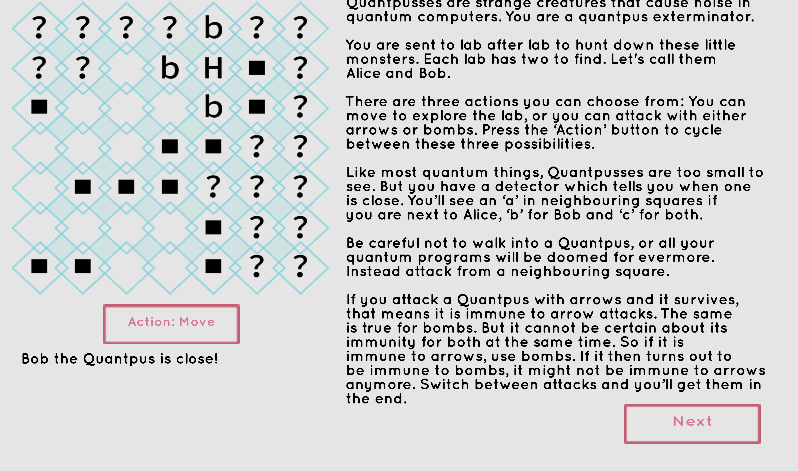
\includegraphics[width=1\textwidth]{Immagini troppo complicate/hunt_the_quantupus.png}
\end{center}
\caption{\scriptsize Screenshot di una partita a Hunt the Quantupus\cite{wootton_quantupus}}\label{fig:img_quantupus}
\end{figure} \\

\newpage
\subsection{Quantum Supremacy e Quantum Awesomeness}
Un tema oggi attualissimo nell'ambito del Quantum Computing è la cosiddetta \emph{Quantum Supremacy}, ovvero la dimostrazione che i computer quantistici sono in grado di fare calcoli che nessun altro computer classico sarebbe in grado di fare in tempi utili\cite{wiki:Quantum_supremacy}. L'argomento, estremamente affascinante quanto complicato, richiede tuttavia sia strumenti astratti che fisici per poter essere studiato ed elaborato, pertanto non c'è da stupirsi nel sapere che i principali studi in questo ambito sono condotti da IBM e Google. Per poter risolvere questa diatriba basterebbe pertanto trovare un problema che può essere affrontato facilmente con un computer quantistico e computazionalmente intrattabile per uno classico. Sebbene ci siano state più proposte di problemi con queste caratteristiche nel tempo, quello più interessante risulta essere il \emph{Random Circuit Samplig}, in breve \emph{RCS}. Un problema infatti ancora irrisolto è quello di trovare un generatore di numeri casuali. Esistono infatti generatori di numeri \textbf{pseudo}-casuali, che partendo da un valore chiamato \emph{seme} generano una sequenza arbitrariamente lunga di numeri. La generazione di questi numeri segue tuttavia una procedura matematica ben definita e deterministica, che se scoperta, assieme al seme, permette di risalire all'intera sequenza pseudo-casuale generata (per maggiori informazioni si veda il Capitolo 4 di \cite{elementi_di_crittografia}). Tutto questo però è un problema dei computer classici. Quelli quantistici, di contro, posta l'assenza di rumore che è probabile raggiungeremo in un non troppo lontano futuro, e la natura dei qubit, che con l'applicazione di determinate porte possono trovarsi in stati di sovrapposizione $\ket{\phi}$ a metà tra lo stato $\ket{0}$ e $\ket{1}$, possono permetterci di creare veri e propri \emph{generatori di numeri \textbf{casuali}}. Da qui nasce il problema RCS: lo scopo è quello di costruire un circuito quantistico in maniera casuale, ovvero applicando porte quantistiche a caso a qubit scelti altrettanto a caso (non importa quanto sia casuale questa procedura), e poi misurare i vari output dal programma. Se il circuito è veramente un circuito quantistico, alla fine ogni output ottenuto dovrebbe avere circa la stessa probabilità di essere misurato. Di fatto risolvere questo problema in tempo utile equivarrebbe a costruire un generatore di numeri casuali efficiente. Nulla vieta di simulare un circuito quantistico su una macchina classica per raggiungere questo scopo, ma quanto sarebbe efficiente tale simulazione? Molto poco, dato che la simulazione di un circuito quantistico su una macchina classica comporta ha un peggioramento esponenziale della sua complessità sia temporale che spaziale. Se riuscissimo quindi a implementare un circuito RCS su una macchina quantistica ottenendo velocemente misurazioni dell'output, avremmo risolto il problema della Quantum Supremacy.
Google aveva già dichiarato, nel 2016, di voler dimostrare la Quantum Supremacy risolvendo il problema RCS usando un chip a 49 qubit capace di campionare distribuzioni di output inaccessibili ai computer classici in un tempo ragionevole. Nell'ottobre del 2019 pubblicò i suoi risultati su un articolo di Nature\cite{nature_quantum_supremacy_google}, avendo sviluppato un processore a 53 qubit chiamato ``Sycamore'' capace di risolvere il problema di meno di quattro minuti, laddove, a loro dire, con un supercomputer classico sarebbero stati necessari 10.000 anni. Quest'ultima affermazione sarebbe poi stata contestata dall'IBM, affermando che un algoritmo classico efficiente sarebbe stato capace di risolvere il problema in due giorni e mezzo sullo stesso dispositivo classico.
In mezzo a tutto questo troviamo James Wootton, che ad agosto del 2017 decise di sviluppare \epmh{Quantum Awesomeness}\cite{wootton_puzzle}\cite{wootton_puzzle_2}, un videogioco con lo scopo sia di facilitare e rendere più stimolante la comprensione del problema della Quantum Supremacy, sia di fungere da campo di prova per i device quantistici, così da testarne le capacità. Prendiamolo alla lontana per capirne la natura.
Dato un computer quantistico, Quantum Awesomeness punta a verificare quanti qubit sono presenti in tale macchina, qual è la sua connettività, ovvero quante porte controllate posso applicare in un circuito arbitrario prima che il rumore renda i risultati insensati, e quanto questa riesce a tenere sotto controllo il rumore stesso. Ricordiamo che una porta controllata è una porta che collega due qubit, dove uno funge da controllo e l'altro da target. Allo stesso tempo, Quantum Awesomeness ci permetterà di creare circuiti RCS e verificarne la qualità, ovvero se ci sono qubit il cui esito è sempre prevedibile. Quindi, dato un computer quantistico a $n$ qubit:
\begin{enumerate}
    \item Vengono scelte alcune coppie di qubit casuali, e a ciascuna di queste viene applicata una \emph{porta C-NOT parziale}, che ricordiamo dal Capitolo 1 essere porte dove al qubit di controllo viene applicata prima una porta $R_x(\phi)$, con $\phi \neq \frac{\pi}{2}$, che lo pone in uno stato di sovrapposizione tra $\ket{0}$ e $\ket{1}$, e poi una porta \emph{C-NOT} che ha come target l'altro qubit della coppia. Ricordiamo inoltre che in questo modo, per entrambi i qubit, la probabilità di misurare 1 può essere più o meno elevata rispetto a quella di misurare 0 (dipende dall'angolo $\phi$ scelto), ma tutte le volte che il qubit di controllo viene misurato 0 (parimenti per 1), lo stesso accade per quello target, e viceversa. L'unico vincolo qui sta nel numero di coppie che possiamo avere: deve essere strettamente minore di $\frac{n}{2}$.
    \item Costruiamo un grafo a partire dal circuito nel modo seguente:
    \begin{itemize}
        \item Ad ogni qubit facciamo corrispondere un nodo.
        \item Dopo aver eseguito il circuito per un certo numero di volte, ad esempio 1024, sapremo con che probabilità ciascun qubit ha dato 1 al momento della misurazione. Riportiamo, nel nodo corrispondente, questa esatta probabilità, come un numero reale che può assumere un valore da 0 a 100 (potevamo anche riportare direttamente il numero ottenuto, la scelta di convertirlo in percentuale è arbitraria). A questo punto, per maggiore leggibilità dell'utente, possiamo anche far corrispondere un colore a ciascun nodo dipendente da questa probabilità. Per esempio, un nodo sarà tanto più rosso quanto più la sua probabilità è vicina allo 0, mentre diventerà bluastro quando questa probabilità si avvicina al 100\%.
        \item Possiamo, per rendere la figura più leggibile all'utente, fissare anzitempo le \emph{possibili} coppie di qubit a cui applicare una porta controllata. Per esempio, potremmo fissare il vincolo che al terzo qubit può essere applicata, in un qualunque momento, una porta controllata dove il secondo qubit coinvolto può essere solo uno tra il secondo, il quarto e il sesto. Ripetiamo, questo vincolo aggiuntivo è da applicare solo se vogliamo costruire un grafo più leggibile per l'utente, ma non è necessario per giocare. Basta solo, nel caso lo si volesse applicare, decidere all'inizio tutte le possibili coppie di qubit, così da non introdurre nei livelli successivi nuovi archi.
        \item Per ogni coppia di nodi costruiamo un arco che li colleghi, identificato dai suoi estremi e dal suo peso. Su ogni arco infatti va riportata la probabilità che i due qubit relativi ai nodi che collega abbiano dato valori diversi dopo la misurazione. Riprendiamo l'esempio delle 1024 esecuzioni. Supponiamo che il secondo qubit del nostro circuito sia stato misurato come 1 per 256 volte, mentre il quinto addirittura 1024. Ciò vuol dire che il numero di volte in cui si sono trovati in disaccordo è $1024 - 256 = 768$, che è il 75\% di 1024. Dunque nell'arco che collega i nodi relativi al secondo e quinto qubit va riportato il valore 75.
    \end{itemize}
    \item Mostriamo il grafo all'utente, chiedendogli di trovare le coppie di qubit che sono state poste in entanglement tra loro. Due qubit in questo stato infatti saranno tali per cui tutte le volte che la misurazione di uno ci ha restituito 1, lo ha fatto anche l'altro. Per trovarle pertanto bisogna cercare i nodi (collegati da un arco) il cui numero (o equivalentemente colore) è uguale, o alternativamente le coppie collegate da un arco il cui valore è 0 (perché ciò vorrebbe dire che i due qubit non si sono mai trovati in disaccordo).
    \item L'utente, dopo aver osservato il grafo e comunicato alla macchina le coppie che secondo lui erano in entanglement, provoca una modifica del circuito. Infatti, per ogni coppia che era effettivamente in entanglement a causa dell'applicazione di una porta \emph{C-NOT} parziale e che l'utente ha segnalato come tale, viene riapplicata la stessa porta, che per il fenomeno della uncomputation fa sì che i due qubit tornino allo stato iniziale, che tipicamente è $\ket{0}$. Se però una coppia era in entanglement e l'utente non se n'è accorto, allora non viene fatta, per quella porta, l'uncomputation, e i due qubit rimangono legati per il resto della partita. Se allo stesso modo il giocatore indica due qubit come entangled quando invece non lo erano, verrà applicata una porta \emph{C-NOT} parziale a questa coppia, rendendoli quindi entangled.
    \item A questo punto il livello corrente è completato, e si passa al successivo ricominciando dal passo 1, con la differenza però che, a causa di un possibile errore dell'utente, qualche coppia di qubit potrebbe essere ancora legata. Ciò andrà a complicare la partita del giocatore, perché se uno di questi qubit viene posto nuovamente in entanglement con un altro, non sarà così semplice accorgersene. Una volta che il giocatore non riesce più a trovare neanche una coppia di qubit in entanglement, il gioco termina. Lo scopo è pertanto quello di superare più livelli possibile prima di raggiungere l'inevitabile \emph{Game Over}.
\end{enumerate}
Abbiamo dunque spiegato le regole del gioco. Vediamo ora come questo si lega all'RCS e a una valutazione qualitativa di un computer quantistico.
\begin{itemize}
    \item Lo scopo dell'RCS, come già detto, è quello di creare un circuito quantistico tale per cui ogni output abbia \textbf{circa} la stessa probabilità di uscire rispetto a qualunque altro possibile output. La parola ``circa'' qui gioca un ruolo fondamentale, perché nel momento in cui riusciamo a eliminarla del tutto vuol dire che abbiamo ottenuto un circuito con una distribuzione di probabilità uniforme degli output, dove nessuna stringa di bit misurata alla fine è favorita rispetto alle altre: hanno tutte la stessa identica probabilità di essere misurate. Per capirci meglio, se abbiamo ad esempio un circuito quantistico a 4 qubit, le possibili stringhe di bit diverse tra loro che possiamo misurare sono $2^{4}$. Nel momento in cui eseguiamo il circuito, per esempio, per 1024 volte, e otteniamo ciascuna di queste 16 stringhe diverse esattamente 64 volte, possiamo dire di aver costruito un piccolo generatore di numeri casuali. Ora, forse con 4 qubit è anche facile costruire un circuito che, almeno teoricamente, produce una distribuzione di probabilità perfetta come quella che abbiamo descritto. Ma sarebbe più interessante avere stringhe di bit molto più lunghe di così. Come facciamo quindi a costruire un circuito quantistico a tanti qubit che rispetti queste proprietà? Insomma, come facciamo ad essere sicuri che gli output prodotti da esso seguano una distribuzione di probabilità come quella desiderata?\\
    È proprio qui che entra in gioco Quantum Awesomeness, che ci permette di costruire un circuito del genere se facciamo una partita non con lo scopo di vincere, \emph{ma con quello di perdere con assoluta certezza}. L'idea è la seguente: iniziamo una partita, dove al primo round avremo una serie di coppie di qubit in entanglement tra loro. Il nostro scopo è sempre quello di trovare tali coppie, ma una volta fatto ciò faremo finta di non averle viste, e procederemo al livello successivo. Questo farà sì che non venga fatta l'uncomputation di alcuna porta. Ripetiamo questo procedimento fino a quando non arriviamo a un livello avanzato in cui:
    \begin{enumerate}
        \item Nessun nodo riporta il valore 0 o 100. Questo vuol dire che tutti i qubit hanno una probabilità diversa da 0 sia di misurare 0 che 1, ovvero, ogni qubit è in entanglement con almeno un altro.
        \item Non riusciamo più a identificare con certezza coppie di qubit in entanglement tra loro. Se si verifica questa situazione vuol dire che abbiamo accumulato così tanti errori durante la partita da rendere il gioco impossibile da proseguire, raggiungendo quindi il Game Over. E questo ci piace molto, perché vuol dire che abbiamo creato un circuito dove non è prevedibile l'esito della misurazione di alcun qubit.
    \end{enumerate}
    Quindi con Quantum Awesomeness la creazione di circuiti RCS davvero casuali è misurabile a occhio nudo: basta controllare se è possibile riconoscere qubit legati tra loro, e nel caso ciò sia vero vuol dire che il circuito non è abbastanza casuale, e vanno applicate ulteriori porte.
    \item Perdere di proposito però non sembra molto stimolante. Fortunatamente anche impegnarsi per cercare di portare avanti una partita e battere il record del mondo comporta dei vantaggi che non riguardano solo il mero orgoglio personale. Uno dei problemi più sentiti ad oggi riguardo i computer quantistici, come detto nel Capitolo 1, è la inevitabile presenza di rumore, che diventa sempre più importante durante l'esecuzione di un programma quantistico col passare del tempo. È proprio per colpa del rumore infatti se ad oggi non riusciamo a mantenere in esecuzione un circuito quantistico per periodi di tempo troppo lunghi, ottenendo risultati paradossali come un qubit che quando misurato, ogni tanto, restituisce lo stato 1 pur essendo, almeno in teoria, sicuramente nello stato $\ket{0}$. %non essendo mai passato attraverso una porta di alcun tipo. 
    Fattori come il numero di qubit coinvolti nella computazione o la quantità di porte a due o più qubit applicate nel circuito non fanno altro che amplificare gli effetti nocivi del rumore. Quantum Awesomeness interviene in questo panorama fornendoci un modo divertente e intuitivo di misurare la capacità di un arbitrario dispositivo quantistico di gestire il rumore. Nel caso di assenza di quest'ultimo, giocare numerosi round di fila sarà estremamente facile, perché sarà sempre possibile, per un giocatore esperto e competitivo (ovvero interessato a vincere più livelli possibile) trovare le coppie di qubit giuste in un dato round. Tanto più invece questo è presente, tanto più il grafo prodotto ad ogni turno ci sembrerà costruito a caso, poiché qubit posti in entanglement non avranno la stessa identica probabilità di misurare 1 né tanto meno andranno d'accordo nel 100\% dei casi, avendo quindi sull'arco che li collega un valore diverso da 0. Per avere un idea grafica di quello che stiamo dicendo si veda la Figura 3.2.
    Pertanto, per verificare la qualità di un dispositivo quantistico, tutto ciò che dobbiamo fare è provare a farci girare sopra Quantum Awesomeness e fare una partita, vedendo quanto a lungo riusciamo a giocare prima che il rumore renda il grafo costruito durante un certo round illeggibile (sottolineiamolo ancora: illeggibile non a causa di errori del giocatore, ma del rumore prodotto dalla macchina. Se vogliamo, possiamo dire di essere nel caso opposto rispetto a quello dei circuiti RCS: lì avevamo come obiettivo quello di far giocare un incompetente, qui invece vorremmo avere il campione del mondo!). Tanti più nodi avrà il grafo, tanto più saranno sofisticati i suoi archi e tanto più sarà il tempo di gioco che avremo a disposizione, tanto più avremo davanti un computer quantistico di qualità. \emph{Google e IBM, fatevi sentire!}
\end{itemize}

 \begin{figure}[h!]
    \captionsetup{font=scriptsize}
    \begin{center}
        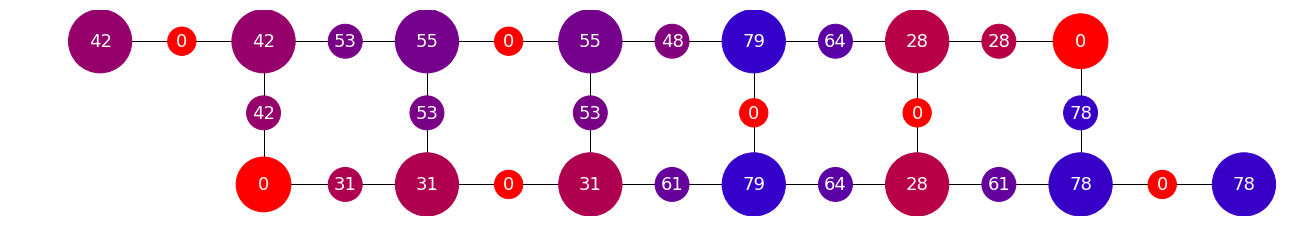
\includegraphics[width=1\textwidth]{Immagini troppo complicate/puzzle_quantum_example_1.png}
        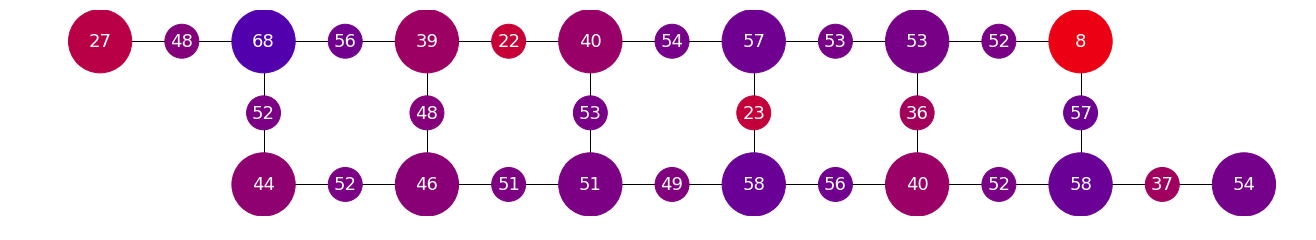
\includegraphics[width=1\textwidth]{Immagini troppo complicate/puzzle_quantum_example_2.png}
    \end{center}
    \caption{\scriptsize Esempio di grafi costruiti a partire da un circuito quantistico a 14 qubit. Sopra, il grafo ottenuto dopo aver eseguito per 1024 volte su un simulatore (esente quindi da rumore) il circuito quantistico. Sotto, il grafo costruito a partire dallo stesso circuito eseguito per 1024 volte su un vero computer quantistico, dove il rumore ha cambiato, a volte anche pesantemente, i valori dei nodi e degli archi. \cite{wootton_puzzle}\cite{wootton_puzzle_2}}\label{fig:img_puzzle_quantum}
\end{figure}
\noindent C'è una piccola nota a margine che dobbiamo fare per quanto riguarda il problema RCS. Sicuramente Quantum Awesomeness è capace di generare circuiti quantistici dove l'esito della misurazione è completamente casuale. Ma se il nostro obiettivo è avere una sorgente di numeri casuali, perché non usare semplicemente delle porte Hadamard? Sappiamo infatti che queste porte, prendendo un qubit in uno stato di base computazionale, lo portano in uno stato di ugual sovrapposizione, dove cioè abbiamo la stessa probabilità di misurare 0 o 1. Quindi perché non usare un circuito a $n$ qubit dove semplicemente applichiamo a ciascuno di loro una porta di Hadamard e poi misuriamo il risultato? O meglio ancora, misuriamo per $n$ volte lo stesso qubit preparato nello stato $\ket{+}$? Questa è una strada sicuramente percorribile, ma come ogni cosa ha i suoi pro e i suoi contro.\\
Sicuramente l'ultimo approccio proposto è quello più economico in termini di risorse: ci bastano un qubit e una porta di Hadamard, e possiamo ottenere stringhe di numeri casuali lunghe quanto ci pare. Tuttavia l'applicazione di una porta di questo tipo richiede che il qubit, supponiamo inizializzato nello stato $\ket{0}$, venga ruotato di $\frac{\pi}{2}$ radianti rispetto all'asse X. Qualunque sia l'implementazione della porta su una macchina quantistica, è probabile che a un certo punto venga richiesto dal dispositivo l'angolo di rotazione, che sarà espresso in maniera classica, ad esempio come numero in virgola mobile. Essendo però questi angoli spesso una frazione di $\pi$, che è già un numero irrazionale, i numeri che li rappresentano saranno per forza di cose una loro approssimazione\cite{random_hadamard}. Quello che potrebbe accadere insomma è che, pur applicando una porta di Hadamard, potremmo, a causa del fatto che non siamo in grado di rappresentare in maniera esatta numeri irrazionali, effettuare una rotazione non di 90°, ma di un valore ad esso molto vicino, per esempio 89,9° o 90,1°. Anche se su carta queste cifre sembrano irrisorie, non dobbiamo dimenticarci che lo scopo finale del problema RCS è proprio quello di generare numeri nella maniera più casuale possibile, per poi applicarli in ambiti in cui anche differenze minuscole come queste contano, ad esempio la crittografia. Infatti un ipotetico crittoanalista che conoscesse l'hardware quantistico usato per generare bit casuali nella maniera appena descritta, potrebbe sfruttare questa imprecisione a suo vantaggio per decifrare degli eventuali crittogrammi. Inoltre gli stessi qubit potrebbero essere imperfetti, a seconda della loro implementazione fisica, e pertanto perfino il processo di inizializzazione nello stato $\ket{0}$ potrebbe essere soggetto a imprecisioni. Sommando tutti questi fattori ci rendiamo conto che, sebbene questo approccio sia il più semplice da adottare e su buoni computer quantistici produca dei risultati più che soddisfacenti, in generale non è una soluzione definitiva al problema RCS.\\
La strada percorsa da Quantum Awesomeness, allo stesso modo, ha pregi e difetti. Innanzitutto non è di così facile attuazione come quella precedente. Richiede device quantistici capaci di gestire numerosi qubit, porte e in grado di svolgere calcoli per periodi di tempo relativamente lunghi, abbastanza da permettere a un giocatore di concludere una partita creando il maggiore caos possibile. Ad oggi quindi questo approccio è indubbiamente più costoso di quello basato sulla porta di Hadamard per molti computer quantistici. Tuttavia il livello di casualità di cui è capace è, in linea di principio, maggiore rispetto a quello del suo concorrente. Ci sono vari elementi di aleatorietà che intercorrono in una partita di Quantum Awesomeness: la scelta delle coppie possibili, gli angoli di rotazione scelti per ciascuna porta $R_x$ applicata e le misurazioni stesse dei qubit una volta giunti al Game Over. Tutti questi elementi possono portare a una maggiore imprevedibilità dei risultati. Usiamo il condizionale perché tutto sta nel come si decidono le possibili coppie e gli angoli delle porte. Se usassimo un generatore di numeri pseudo-casuali classico a questo scopo correremmo qualche rischio, in quanto un crittoanalista potrebbe risalire a questi generatori e avere informazioni parziali sulla struttura del circuito. È tuttavia vero che se, per esempio, avessimo bisogno di generare 1024 bit casualmente, potremmo fare $k$ partite a Quantum Awesomeness dove ogni volta otteniamo $\frac{1024}{k}$ bit, impiegando per ogni esecuzione un seme diverso per il nostro generatore. Oppure potremmo, anziché cercare subito il Game Over, prolungare la partita azzeccando, nel corso dei round, alcune coppie, così da annullare porte precedentemente applicate e lasciare spazio a nuove combinazioni: un crittoanalista a quel punto non avrebbe modo di sapere come abbiamo giocato. Oppure potremmo applicare generatori di coppie e angoli ``fisici'', ad esempio mettendo dei banalissimi pezzi di carta in un sacchetto, dove su ciascuno di essi è trascritta una possibile coppia di qubit o un angolo in radianti, e pescare alla cieca elementi da esso. In conclusione, Quantum Awesomeness propone una soluzione al problema RCS più complicata da implementare con i mezzi odierni, ma che ha svariati assi nella manica da giocarsi per assicurare una generazione casuale di bit.\\
\subsection{Il primo Quantum Game Jam}
A febbraio del 2019 troviamo un ulteriore evento storico per i videogiochi quantistici, al quale ovviamente non è mancato James Wootton, anche se stavolta più in veste di tutore: il \emph{Quantum Game Jam} di Helsinki\cite{wootton_helsinki}. Con \emph{Game Jam} si intende una competizione tra programmatori, game designers e simili, dove ogni gruppo di sviluppatori ha il compito di partorire un videogioco in un lasso di tempo che va dalle 24 alle 72 ore. Occasioni del genere servono a mettere alla prova la creatività, bravura e conoscenza dei partecipanti, stimolandoli a migliorare e, se il gioco è di buona fattura, anche a farsi pubblicità. La particolarità di questo Game Jam sta nel fatto che tutti i videogiochi prodotti avrebbero dovuto in qualche modo incorporare nelle loro meccaniche di gioco un aspetto della fisica quantistica. Come campo di prova, i partecipanti avrebbero avuto dei simulatori e dei veri computer quantistici forniti dall'IBM su cui far girare le proprie creazioni. Visto che uno dei principali studi nell'ambito del quantum computing riguarda la riduzione del rumore, è stato chiesto ai presenti di pensare come incorporare questo particolare effetto nelle meccaniche di gioco. E quello che più di tutti ha preso alla lettera questo consiglio è stato $Q\ket{Cards}$, un gioco di carte atto ad insegnare ai partecipanti le basi del quantum computing. L'idea era quella di simulare nel gioco l'esecuzione di un circuito che poi sarebbe stato mandato in esecuzione su una vera macchina. Ogni giocatore avrebbe avuto, a inizio partita, un personalissimo qubit e una mano di carte. Lo scopo era quello di giocare le giuste carte nel giusto ordine nel corso della partita, dove ogni carta corrisponde ad una trasformazione applicata al proprio qubit. Segnandosi l'ordine e il tipo delle giocate, sarebbe stato possibile costruire un circuito quantistico da mandare in esecuzione su un simulatore o su una macchina quantistica. Se l'esecuzione nel simulatore non fa altro che rispecchiare l'esito della partita, nel caso di esecuzione su computer quantistico abbiamo una dimensione aggiuntiva nel gameplay. Infatti, a causa del rumore, fino all'ultimo non è possibile stabilire quale sarà il qubit vincitore. In tal caso, la strategia dei giocatori avrebbe dovuto tenere di conto di questa variabile, che li avrebbe portati a fare talvolta giocate più sicure (meno rumorose) ma meno vantaggiose, talvolta giocate più audaci (più rumorose) ma che avrebbero potuto portare più vicini alla vittoria. Ancora una volta, notiamo come la casualità fornitaci dai dispositivi quantistici sia estremamente invitante per i game designers che progettano un elemento di aleatorietà nel loro gioco. Ed è infatti proprio sulla capacità di questi dispositivi di fungere da random number generators che si basano altri due giochi del Game Jam, \emph{Qubit Gardener} e \emph{SneaQysnake}. Nel caso di Qubit Gardener abbiamo un rilassante passatempo, dove il nostro unico scopo è quello di annaffiare un giardino per vederne nascere i fiori. La particolarità sta nella vera generazione casuale delle piante, dove sia l'immagine sulla corolla che il colore e la forma dei petali sono generati casualmente. Molti giochi odierni, come Minecraft\cite{wiki:Minecraft}, attuano un processo di generazione procedurale del mondo, dove è praticamente impossibile avere due volte la stessa mappa da esplorare. Tuttavia gli ambienti che vengono generati diventano riconoscibili dopo una decina di partite: si tratta sempre delle stesse pianure, delle stesse miniere abbandonate e degli stessi villaggi con le stesse case, dalle quali si impara cosa aspettarsi. Con una generazione realmente casuale del mondo di gioco, però, ogni partita avrebbe sempre un elemento non riscontrabile altrimenti. SneaQysnake, una versione quantistica del famoso \emph{Snake}, allo stesso modo, sfrutta questa casualità per generare il prossimo frutto che il serpente dovrà mangiare in un luogo imprevedibile.
L'ultimo gioco prodotto durante questo Game Jam che citiamo è \emph{Qubit the Barbarian}, gioco in stile roguelike\cite{wiki:Roguelike} basato sulla misurazione di più qubit. Vestendo i panni di un barbaro esploratore, il nostro obiettivo è quello di esplorare una caverna sotterranea a più piani popolata da nemici, alla ricerca della chiave che permette di sbloccare le scale e scendere al piano successivo, il tutto cercando cibo che ci impedirà di morire di fame. La particolarità di questo prodotto videoludico sta nel fatto che ogni casella della grotta è associata a un qubit preparato in uno stato di base computazionale scelto a caso tra la base X, Y o Z, e il barbaro, in un qualunque momento della sua esplorazione, può decidere di effettuare la misurazione delle caselle (qubit) adiacenti in una di queste tre basi. Facendo una misurazione di una casella, questa può far sparire il muro che aveva sopra di sé, può farne comparire uno se prima non c'era o può non cambiare affatto, permettendo al giocatore di creare un percorso che lo porti alla destinazione desiderata. Pur essendo a livello di concept e di grafica molto rudimentale, \emph{Qubit the Barbarian} ci dà un'idea di come un gioco quantistico del futuro potrebbe basare alcune delle sue meccaniche su peculiarità del quantum computing. Da quest'idea potrebbero nascere nuovi puzzle-game dove il giocatore deve trovare un pattern tra più elementi di gioco associati a qubit, scovando la base computazionale con cui sono stati preparati così da fare le giuste misure nel giusto ordine e raggiungere lo stato desiderato. Non solo, ma con questo gioco ci viene anche mostrato come il calcolo quantistico possa essere usato anche solo per compiere particolari operazioni in background, lontano dagli occhi del giocatore. Pur non conoscendo le basi computazionali, infatti, un qualunque giocatore può imparare con l'esperienza il funzionamento dei vari comandi, arrivando a muovere i muri circostanti a proprio piacimento.
\begin{figure}[H]
\captionsetup{font=scriptsize}
\begin{center}
    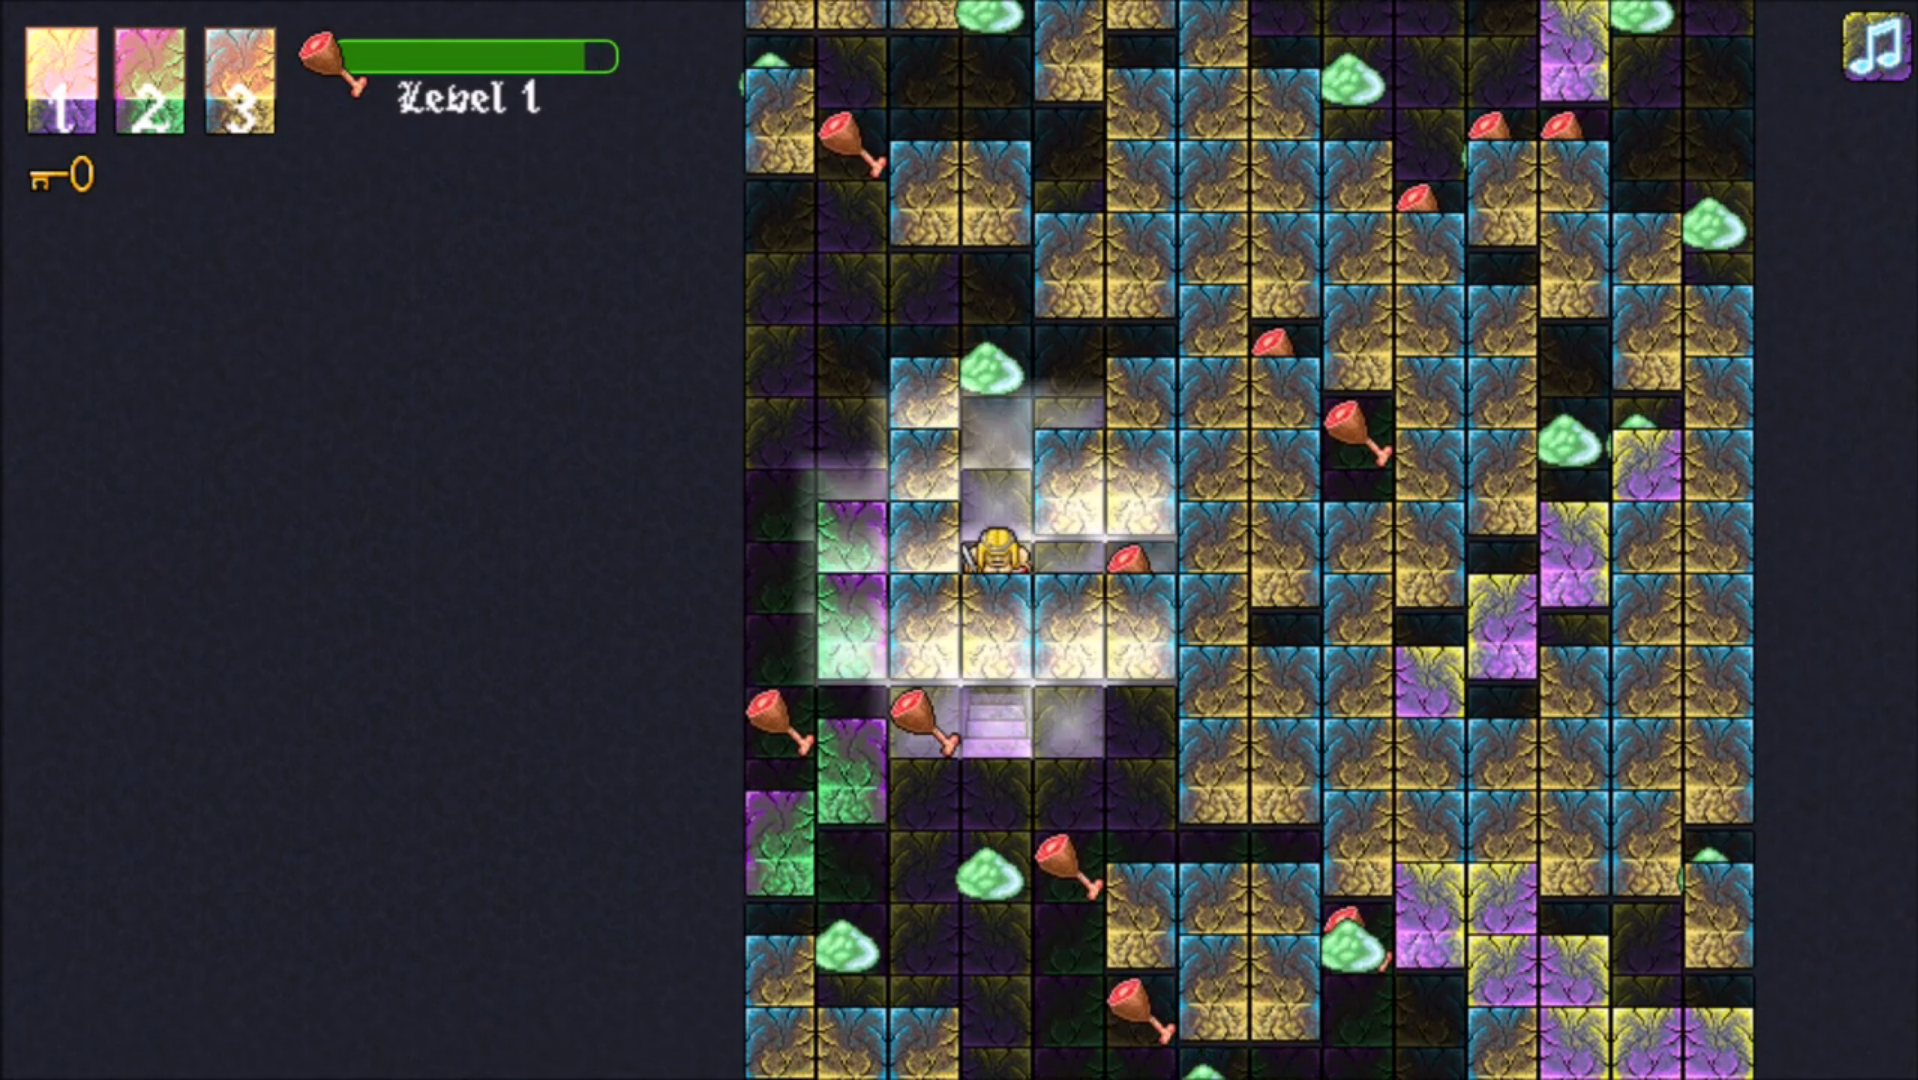
\includegraphics[width=0.73\textwidth]{Immagini troppo complicate/qubit_the_barbarian_screenshot.png}
\end{center}
\caption{\scriptsize Screenshot di una partita a Qubit the Barbarian\cite{wootton_puzzle}}\label{fig:img_qubit_the_barbarian}
\end{figure}

\subsection{Generazione di mondi casuali}
Abbiamo già sottolineato più volte come uno dei principali vantaggi che possiamo ottenere utilizzando macchine quantistiche al posto di quelle classiche è la creazione di un vero random number generator, dove i valori prodotti sono realmente casuali. Questo apre le porte, nel mondo del gaming, a una enorme quantità di possibilità che oggi ci sono proibite. Di fatto sono moltissimi i videogiochi moderni che basano la propria difficoltà e rigiocabilità su processi stocastici. Il famoso roguelike \emph{The Binding of Isaac}\cite{wiki:The_Binding_of_Isaac:_Rebirth} garantisce infatti migliaia di ore di gioco riempite di partite sempre differenti grazie a una generazione pseudo-casuale di mappe. L'idea fondamentale è che, dato un insieme di possibili stanze, oggetti, vincoli sulla dimensione della mappa e un \emph{seed} iniziale, tipicamente una stringa a otto caratteri, il gioco è in grado di generare ogni volta un mondo da esplorare diverso da tutti quelli precedenti, garantendo un'esperienza sempre diversa al giocatore. Ciò nonostante, dopo svariate ore di gioco, si comincia ad intravedere un pattern: le stanze sono sempre le solite, popolate dagli stessi nemici che si trovano sempre nella medesima posizione e che compiono un numero predefinito di mosse. Lo stesso principio si applica a tutti i giochi del genere anche se in salsa leggermente diversa. Il più recente \emph{No Man's Sky}\cite{wiki:No_Man's_Sky} aveva fatto molto parlare di sé al momento del suo lancio, anche se per i motivi sbagliati. Il gioco prometteva infatti una generazione completamente procedurale dei suoi contenuti, a partire dai pianeti esplorabili fino alle creature che li abitavano. Di fatto però dopo qualche decina di ore di gioco si cominciavano a riconoscere le stesse strutture poste in ambienti diversi, le stesse specie, gli stessi consumabili. Insomma, la generazione casuale era sì presente, ma non in modo innovativo come invece sembrava dalle presentazioni antecedenti al lancio. La domanda che ci poniamo è pertanto: è possibile usare i computer quantistici per avere una generazione casuale di contenuti in un gioco? E perché non possiamo raggiungerla con mezzi classici?\\
Tutte le volte che vogliamo produrre in modo casuale un puzzle, un livello o una mappa, dobbiamo scontrarci con una serie di vincoli difficili da soddisfare. Ad esempio vogliamo che i puzzle generati siano risolvibili, i livelli battibili e le mappe prive di trappole, ovvero zone che, se accedute, non permettono di tornare indietro. Un altro vincolo meno matematico che dobbiamo soddisfare è che il contenuto generato sia stimolante per il giocatore. Infatti nessuno vuole mettersi a risolvere un puzzle troppo facile o difficile, sia questo anche generato casualmente e munito di una soluzione. In linea di principio un gioco dovrebbe quindi generare casualmente un livello e verificarne in tempo reale la soddisfacibilità e ludicità. Ma un'operazione del genere può richiedere tempi esosi ai dispositivi classici. Si pensi ad un semplice gioco dove, dato un insieme di città collegate da strade di costo variabile, si chiede al giocatore di trovare il percorso minimo che le attraversi tutte una volta soltanto. Il gioco, per poter verificare la qualità della soluzione proposta, dovrebbe prima trovare da sé quella ottima. Trattandosi però del problema del commesso viaggiatore, famoso per essere un problema computazionalmente difficile da risolvere con mezzi classici, non possiamo aspettarci che il software di gioco riesca a trovarne la soluzione in tempi ragionevoli. Qui entra in gioco la computazione quantistica, che ci permetterebbe di trovare il percorso minimo con uno speedup polinomiale. Allo stesso tempo, i computer quantistici potrebbero essere usati non solo per verificare velocemente la soddisfacibilità di problemi generati casualmente, ma anche di generarli loro stessi. A dare una primo algoritmo per la generazione casuale di terreni di gioco con queste caratteristiche ci pensa come sempre James Wootton in un suo articolo\cite{wootton_random_world}, dimostrandoci come il mondo dei contenuti generati casualmente sia non vicino, ma già disponibile. Dovremo tuttavia attendere ulteriori sviluppi degli hardware quantistici prima che questi risultati possano essere sfruttati a pieno dai giocatori.

\section{Altri esempi di quantum games}
Con l'avvento di pacchetti software come Qiskit dell'IBM e Cirq di Google che hanno permesso a tutti di costruire e simulare circuiti quantistici usando un semplice linguaggio di programmazione, avendo inoltre la possibilità di mandare in esecuzione i propri programmi su veri computer quantistici, diversi sviluppatori si sono interessati sempre di più al mondo del quantum computing. Con ciò, alcuni game designers indipendenti non hanno tardato a sperimentare nuove tipologie di giochi che potessero sfruttare le peculiarità della meccanica quantistica. Vediamone pertanto alcuni esempi.

\subsection{Quantum Game Chess}
Un caso di videogioco quantistico che ha ottenuto molta popolarità negli ultimi anni è quello degli Scacchi Quantistici, o \emph{Quantum Chess}\cite{quantum_chess}, ideati da Chris Cantwell nel 2014. All'epoca il neo-laureato studente di fisica e game designer cominciò a pensare a un videogioco basato sui principi della meccanica quantistica, capace di insegnare questi ai giocatori in modo indiretto e pratico, così che anche i meno esperti potessero approcciarsi all'argomento in modo intuitivo. Il progetto venne notato dall'\emph{Institute for Quantum Information and Matter (IQIM, California Institute of Technology%, Pasadena, CA, United States
)}, in particolare da \emph{Spiros Michalakis}, che decise di aiutare Chris nel suo progetto. Dopo solo un anno Quantum Chess era pronto, e per pubblicizzarlo venne girato un video, ``\emph{Anyone Can Quantum}'', avente come protagonisti Stephen Hawking e Paul Rudd (attore che ha vestito i panni di \emph{Ant-Man} nell'omonimo film), narrato da Keanu Reeves\cite{paul_rudd_chess}. Il video, dai toni molto ironici, aveva lo scopo di mostrare agli spettatori le meccaniche base del gioco e come, con i mezzi odierni, non sia necessario essere dei geni della fisica per cominciare a lavorare con macchine quantistiche. Il gioco, oggi disponibile sulla nota piattaforma per la vendita di videogiochi \emph{Steam}, venne perfino eseguito su una vera macchina quantistica durante il \emph{Quantum Summer Symposium} di Google del 2020\cite{quantum_chess_demonstration}. Ma come funziona esattamente?\\
Ebbene, cominciamo col dire che tutte le regole degli scacchi classici continuano a valere in questa variante quantistica. L'unica eccezione sta nel fatto che non esiste il concetto di ``scacco matto''. Per concludere una partita bisogna per forza catturare il re avversario. Il motivo di ciò risiede nelle meccaniche quantistiche del gioco, basate sui fenomeni di sovrapposizione, entanglement e misurazione. Ci sono infatti una serie di regole quantistiche aggiuntive che i giocatori possono sfruttare a loro vantaggio:
\begin{enumerate}
    \item Durante il proprio turno, si può effettuare una \emph{mossa quantistica} al posto di quella classica. Per fare ciò, basta scegliere un pezzo diverso dai pedoni, e fargli compiere \emph{due mosse} di fila. Ad esempio, si potrebbe spostare la regina avanti di due caselle e poi a sinistra di tre. Se la regola fosse soltanto questa però ogni giocatore la applicherebbe durante ogni turno. Ma è qui che entra in ballo la prima meccanica di gioco quantistica: \emph{un pezzo mosso in questo modo entra in uno stato di sovrapposizione, dove la probabilità che si sia effettivamente spostato nella casella desiderata diventa la metà della probabilità che si trovasse nella casella di partenza}. Riprendiamo l'esempio della regina di prima per capirci meglio. All'inizio della partita, la regina si troverà con una probabilità pari al 100\% nella sua casella iniziale. Dopo che però è stata eseguita la mossa quantistica, questa si troverà con il 50\% di probabilità nella nuova casella, e con l'altro 50\% di probabilità ancora al punto di partenza. Per visualizzare meglio questo evento possiamo immaginarci che la scacchiera si sia sdoppiata in due: nella prima di queste la regina si è effettivamente mossa avanti di due e a sinistra di tre, nella seconda la mossa non è mai avvenuta, e il giocatore ha di fatto sprecato un turno. Si tratta quindi di una giocata rischiosa ma che può portare a diversi vantaggi, quantificabili solo quando uno di questi pezzi viene \emph{misurato}.
    \item Ma quand'è che effettivamente un pezzo viene misurato? Anche se in questa variante degli scacchi è ammesso che un pezzo si trovi in due caselle distinte in un dato momento grazie al fenomeno della sovrapposizione, continua ad essere proibito, come nella versione normale, che ci siano due pezzi diversi nella stessa casella in contemporanea. Questo vuol dire che se l'avversario decide ad un certo punto di attaccare la regina, prendendo di mira una delle due possibili caselle che potrebbe star occupando, deve essere stabilita la reale posizione di questo pezzo. È qui che avviene la misurazione: nel momento dell'attacco viene stabilita la casella in cui si trova la regina. Se l'avversario ha avuto fortuna e la misurazione ha stabilito che questa si trovava effettivamente nella posizione attaccata, allora verrà catturata. Altrimenti, sarà come se l'avversario avesse mosso il suo pezzo in una casella vuota, e la regina non si fosse mai spostata dalla sua posizione iniziale. Lo stesso accade se un pezzo dello stesso colore della regina decide di muoversi in una casella dove potrebbe trovarsi quest'ultima. C'è tuttavia ancora un fenomeno da considerare, quello dell'\emph{entanglement}.
    \item Immaginiamo di trovarci ancora nella situazione iniziale in cui la regina ha effettuato una mossa quantistica, e che sia il turno del giocatore che l'ha mossa. Negli scacchi normali un pedone non potrebbe superare un pezzo che gli sta di fronte. In questo caso però c'è solo il 50\% di probabilità che la regina si trovi effettivamente davanti al pedone, impedendogli di muoversi. Pertanto, come bisogna comportarsi? Per capirlo, dobbiamo introdurre l'ultima meccanica di gioco quantistica presente: la capacità dei pezzi di entrare in \emph{entanglement}. In questo caso infatti il pedone potrà muoversi avanti di due caselle, ``saltando'' oltre la regina che \emph{potrebbe} trovarsi davanti a lui. Per farlo però deve entrare in entanglement con il pezzo saltato. Questo vuol dire che i ``destini'' dei due pezzi sono ora legati indissolubilmente. Quando infatti dovrà essere misurata la regina o il pedone, lo stesso dovrà avvenire anche per l'altro pezzo. In tal caso avremo una scacchiera in cui o il pedone si è mosso e la regina no, o il pedone è rimasto fermo e la regina si è mossa.
\end{enumerate}
Il motivo per cui quindi è necessario catturare il re avversario per vincere piuttosto che porlo sotto scacco è presto detto: il re potrebbe trovarsi in uno stato di sovrapposizione, e finché non lo si prova a catturare non si può sapere se effettivamente era sotto scacco oppure no. Ci sarebbero poi tutta una serie di scenari da considerare, nel caso si volesse fare una vera partita, come ad esempio capire cosa succede se un pezzo posto in sovrapposizione tenta di catturarne un altro, sia questo a sua volta in sovrapposizione o meno, ma ciò esula dai nostri scopi. I lettori più interessati ad approfondire possono provare il gioco da Steam o cercare su Youtube vari video di partite registrate. Quello che però ci interessa sottolineare è come Quantum Chess riesca a riassumere in maniera elegante un po' tutti gli aspetti dei videogiochi quantistici analizzati fino ad ora: il gioco è capace non solo di presentare i principi della meccanica quantistica in un modo più stimolante e comprensibile anche ai meno preparati, ma li integra al suo interno al punto da:
\begin{enumerate}
    \item Farne le sue meccaniche chiave di gioco
    \item Essere in grado di rendere ancora più realistica l'esperienza facendo decidere a un vero computer quantistico l'esito di una giocata. Ogni pezzo è infatti rappresentato da un qubit, a cui vengono applicate le porte necessarie e che viene misurato nel momento del bisogno.
\end{enumerate}
Ovviamente non chiediamo che un videogioco quantistico del futuro debba per forza far andare a braccetto il lato didattico con quello ludico. Anche se riuscisse ``solo'' a velocizzare calcoli ad oggi lenti come quelli di alcune schermate di caricamento avremmo raggiunto un traguardo di non poco conto. Ciò nonostante, Quantum Chess rimane un esempio di lustro nel panorama dei quantum videogames moderni.

\begin{figure}[h!]
\captionsetup{font=scriptsize}
\begin{center}
    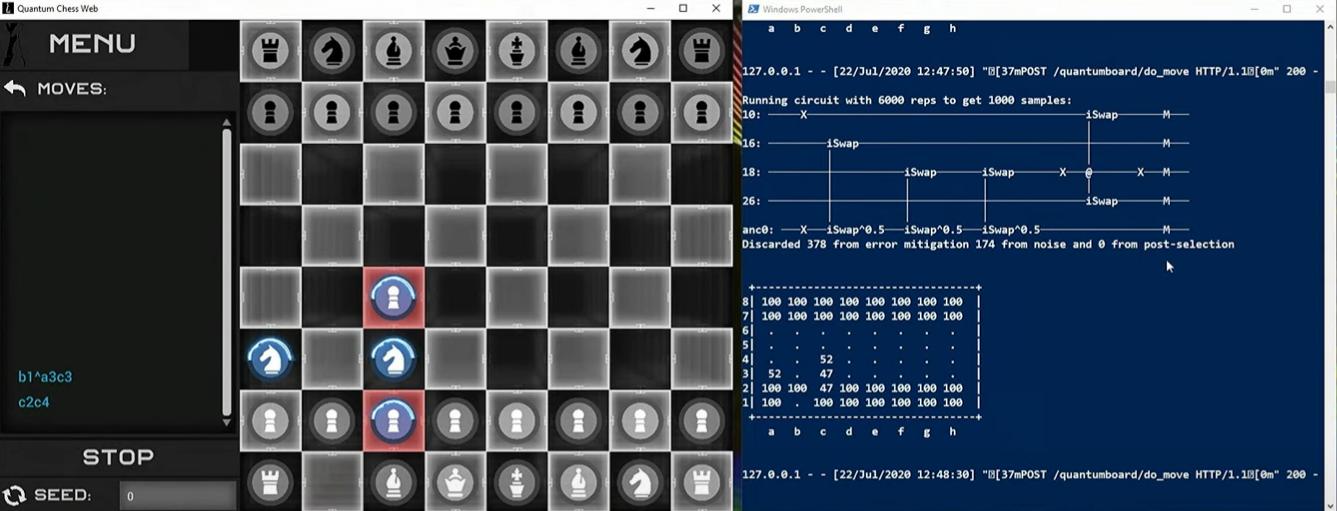
\includegraphics[width=1\textwidth]{Immagini troppo complicate/quantum_chess_google.png}
\end{center}
\caption{\scriptsize Esempio di esecuzione di una partita a Quantum Chess su un computer quantistico di Google\cite{quantum_chess_demonstration}}\label{fig:img_chess_quantum_google}
\end{figure}

\subsection{Quantum Pokémon Fight}
Parlando di come con i mezzi quantistici potremmo riuscire a velocizzare calcoli ad oggi costosi, è stato sviluppato in maniera indipendente un prototipo di intelligenza artificiale quantistica per i videogiochi della saga \emph{Pokémon}\cite{wiki:Pokemon}, a cura di Michaël Rollin\cite{quantum_pokemon_fight}. Tale codice cerca di simulare il comportamento di un allenatore nemico durante uno scontro tra allenatori Pokémon, basato sulle regole fondamentali del gioco, come i rapporti tra i tipi delle mosse e dei mostriciattoli coinvolti. Il primo aspetto quantistico lo troviamo nella generazione casuale dei cosiddetti ``effetti secondari'' che una mossa può generare. Nel mondo del competitivo Pokémon moderno infatti uno dei principali elementi di gioco che rende talvolta le partite impari è la frequenza dei cosiddetti ``\emph{brutti colpi}'', ovvero attacchi critici che si verificano con probabilità del 4.17\%\cite{crit_hit} e che permettono ad una mossa di causare un danno 1.5 volte maggiore del normale. Dato che le strategie dei giocatori più bravi si basano sul calcolo preventivo dei danni che un pokémon può aspettarsi di ricevere quando attaccato, è chiaro che questi colpi critici possono risultare un elemento di aleatorietà piuttosto importante, a volte tale da decidere le sorti di un match. Non è troppo raro vedere partite in cui lo stesso giocatore subisce anche per due o tre volte di fila un brutto colpo, venendo sconfitto. Questo è dovuto anche al fatto che la decisione di applicare questo effetto secondario ad un attacco deriva da un generatore di numeri pseudo-casuali, che nel corso di una partita può creare risultati troppo impari. Se però questo processo di decisione fosse completamente quantistico, come accade nell'articolo di Rollin, allora potremmo aspettarci una distribuzioni di brutti colpi più regolare, riducendo situazioni assurde dove l'esito della partita è determinato unicamente dai colpi critici.\\
L'altro aspetto quantistico trattato riguarda la scelta della mossa da compiere da parte dell'avversario. Per prendere questa decisione viene utilizzato l'algoritmo di ricerca quantistico di Grover. Ricevendo come input le mosse conosciute dal proprio pokémon in campo e le resistenze e debolezze della creatura avversaria, il circuito, composto come al solito da un oracolo e dal diffuser, è in grado di dire se conviene sostituire il mostriciattolo schierato con uno della riserva oppure attaccare con una specifica mossa, quella che risulterà super-efficace sul nemico. Pur essendo solo un prototipo, si potrebbe partire da questa implementazione per sviluppare ulteriori meccanismi di intelligenza artificiale atti a velocizzare processi di scelta all'interno di questi giochi e non solo. Riprendendo l'esempio del competitivo pokémon, un altro problema con cui vari giocatori si scontrano quotidianamente è la scelta delle creature da portare in un match. Quando infatti ha inizio una partita, vengono dati novanta secondi di tempo ai due contendenti per decidere tre o quattro dei sei pokémon della propria squadra da far partecipare all'incontro. Se però il giocatore non effettua questa scelta nel tempo prestabilito, il software renderà automaticamente partecipi i primi quattro pokémon della squadra. Questo meccanismo ha il vantaggio di essere molto veloce, condizione necessaria quando si tratta di lotte on-line, ma altrettanto inefficiente, considerato che spesso le prime quattro creature potrebbero non essere le più performanti per il match corrente. Un circuito quantistico basato su Grover che riceve come input informazioni sui pokémon propri e avversari, tuttavia, potrebbe scegliere velocemente la squadra migliore per la partita corrente. Tali informazioni potrebbero essere elementari, come le tipologie dei vari pokémon coinvolti, portando quindi ad un circuito relativamente semplice da costruire al prezzo di una scelta sub-ottimale, oppure ricche di dettagli complessi, come le statistiche, le abilità, gli oggetti portati e le mosse, costringendoci a costruire un circuito più complicato ma che conduce all'ottimo. 

\section{L'universo quantistico di Outer Wilds}
Fino ad ora abbiamo esaminato vari videogiochi che erano quantistici sia di nome che di fatto. Il loro scopo non era solo quello di insegnare le meccaniche della fisica quantistica in modo accessibile, ma di incorporarle direttamente al loro interno, con la possibilità di essere eseguiti su un vero quantum device. Questa scelta di design ha il vantaggio, se usata in maniera creativa, di essere molto efficace nell'insegnare l'argomento a chi sta muovendo i suoi primi passi in questo mondo tanto complesso quanto affascinante. Tuttavia, è innegabile che un individuo con scarse conoscenze di base sul tema faticherà molto di più a coglierne l'essenza, anche se messo davanti a una scacchiera di Quantum Chess. Questi giochi, legandosi inevitabilmente a un contesto strettamente matematico, potrebbero dunque non catturare l'attenzione del pubblico meno preparato, che però in potenza potrebbe essere interessato ad approfondire tale topic. Purtroppo anche l'occhio vuole la sua parte, e in questo, almeno ad oggi, i quantum games sono un passo indietro rispetto ai videogiochi sviluppati per dispositivi classici, dato che la grafica migliore l'abbiamo riscontrata con la scacchiera 2D di Quantum Chess e con la \emph{pixel art} di Qubit the Barbarian, che impallidiscono di fronte a titoli classici degli ultimi anni. La domanda diventa pertanto: sacrificando l'elemento di rigorosità, è possibile creare videogiochi che girino su macchine classiche ma che diano un'intuizione ai loro giocatori di come funzioni il mondo della fisica quantistica? La risposta è ovviamente sì, e ci sono vari esempi al riguardo. L'esponente che però riteniamo incarni al meglio questa volontà è un titolo uscito nel 2019 dalle geniali menti dello studio \emph{Mobius Digital}\cite{mobius_digital}: stiamo parlando di \emph{Outer Wilds}. Segue adesso una breve introduzione al mondo di gioco, continuata da una trattazione su come questo riesca ad incarnare molto bene gli elementi principali della meccanica quantistica. È chiaro che per poter far ciò bisogna anticipare alcuni dei suoi contenuti, se pertanto siete interessati a dargli uno sguardo ``alla cieca'' vi consigliamo di saltare per il momento questo paragrafo e andare direttamente al prossimo capitolo.\\
In Outer Wilds vestiremo i panni di un \emph{teporiano}, trattasi di una razza aliena appartenente ad un sistema solare diverso dal nostro. L'avventura ha inizio nel villaggio di ``Cuore Legnoso'', l'equivalente della nostra Terra, dove sono partite ormai da anni le Esplorazioni Outer Wilds, ovvero spedizioni nello spazio atte a raccogliere maggiori informazioni sul nostro sistema solare e sull'antica civiltà che vi ha abitato a lungo per poi sparire lasciando poche tracce: quella dei \emph{nomai}. Visitando il museo del nostro villaggio che ci introdurrà alle meccaniche principali di gioco, non potremo fare a meno di passare di fronte a una statua costruita dai nomai stessi che ne raffigura un esemplare, la quale si animerà per qualche secondo di fronte ai nostri occhi, compiendo un gesto che ci cambierà il futuro per sempre.  Di lì a poco avrà inizio la nostra prima spedizione spaziale, che però purtroppo terminerà dopo appena ventidue minuti: allo scadere di questo periodo di tempo il sole esploderà, trasformandosi in una supernova che cancellerà noi e l'intera galassia. Per un motivo a noi sconosciuto, ma che sappiamo essere legato in qualche modo a quella strana statua, verremo catapultati ventidue minuti indietro nel tempo, potendo di fatto ripetere il nostro viaggio tutte le volte che vogliamo... o quasi. Non c'è un obiettivo specifico nel gioco, siamo noi a decidere dove muoverci e quali risposte cercare alle numerose domande che Outer Wilds ci insinuerà nel corso delle nostre spedizioni. Chi erano i nomai? Perché si sono estinti? Perché siamo intrappolati in un loop temporale? Non si può fare nulla per evitare che il sole collassi, cancellando la nostra specie, cultura e tutti coloro che ci sono cari? E qual è il nostro ruolo nell'universo? Solo esplorando i vari pianeti del sistema solare e cercando tracce della civiltà nomai, composte da manoscritti, edifici in rovina e astronavi abbandonate potremo dare una risposta a tutti questi quesiti.\\
Dopo aver svolto un certo quantitativo di esplorazioni ci renderemo conto che i nomai provavano particolare interesse per un'entità, apparentemente un corpo celeste lontano anni luce da noi, chiamata \emph{l'Occhio dell'universo}, che però non sono mai riusciti a raggiungere. Ulteriori studi hanno dimostrato che c'è una correlazione tra l'Occhio e un altro astro che è invece visibile, e teoricamente raggiungibile, dal nostro sistema solare, trattasi della \emph{Luna Quantica}. Tale luna presenta delle proprietà molto particolari. Quando non è osservata da un \emph{osservatore consapevole}, questa è contemporaneamente in orbita sui cinque pianeti che gravitano attorno al nostro sole e sull'Occhio. Quando invece viene osservata, in particolare da noi, questa ``decide'' la sua posizione, e comincia ad orbitare solo attorno ad un pianeta. Qui troviamo la prima meccanica quantistica applicata al mondo di Outer Wilds, ovvero la sovrapposizione: fintanto che la luna non viene misurata da un osservatore consapevole che si mette a guardarla, questa si trova in uno stato di sovrapposizione, che fa sì che sia contemporaneamente in orbita attorno a sei pianeti. Come anticipato l'interpretazione di questo principio (e non solo) è piuttosto romanzata nel gioco, ma è proprio questo il suo elemento di forza, ovvero non fare affidamento su una spiegazione rigorosa del fenomeno ma lasciare che sia l'utente a intuirlo e interiorizzarlo con parole sue. Detto questo, un nuovo giocatore difficilmente riuscirà ad addentrarsi nell'atmosfera di questo corpo celeste, che svanirà davanti ai suoi occhi nel momento in cui proverà ad atterrarvi. E se anche dovesse essere abbastanza fortunato da entrarci provando strategie casuali fino a trovare quella corretta, non riuscirebbe comunque a scoprirne i segreti più profondi. Questo perché egli ancora non conosce tutte le leggi necessarie per l'esplorazione di tale satellite, che però fortunatamente i nomai ci hanno lasciato in luoghi specifici del nostro sistema solare. In particolare, bisognerà visitare la \emph{Torre quantica di sperimentazione}, la \emph{Torre della conoscenza quantica} e la \emph{Caverna Fondolago} per esplorare l'astro a fondo. Le due torri non sono di nostro particolare interesse, dato che introducono regole incentrate più su meccaniche esplorative del gioco che sulla fisica quantistica stessa. %(trattasi della \emph{regola del sesto luogo} (TODO) e la \emph{regola dell'immagine quantistica}, che citiamo solo per completezza).
La Caverna Fondolago tuttavia introduce il concetto dell'entanglement quantistico con la cosiddetta \emph{Regola della correlazione quantica}. In questo luogo troveremo infatti un frammento di Luna Quantica (ce ne sono vari sparsi per il mondo di gioco), con annessi manoscritti dei nomai che raccontano di come grazie ad esso abbiano scoperto una proprietà quantistica piuttosto interessante. Tale caverna è situata nelle profondità di uno dei due pianeti più vicini al sole, \emph{Gemello Brace}, pertanto sarebbe in uno stato di costante oscurità se non fosse per la presenza della nostra torcia. Proprio come accade per la luna, questo oggetto si trova in uno stato di sovrapposizione che lo fa essere contemporaneamente in più luoghi del pianeta, almeno finché non viene osservato attivamente. Allo stesso modo, anche l'assenza di luce costringe ad uno stato di sovrapposizione il frammento, che però può essere misurato se illuminato e posto sotto i nostri occhi. Può dunque balenarci in testa un dubbio: cosa accade se tocchiamo quest'oggetto quando è buio? La riposta è presto detta: entriamo in entanglement con lui. Al momento della riaccensione della torcia il frammento deciderà la sua posizione nel pianeta, facendoci trovare talvolta ``teletrasportati'' all'interno di un'altra caverna. Questa regola ci permetterà, una volta atterrati sulla Luna Quantica, di capirne meglio le proprietà e di esplorarla a fondo. Come abbiamo già detto la luna può essere il satellite di sei corpi celesti differenti, e una volta superata la sua atmosfera (e quindi misurata, perché stiamo letteralmente toccando e osservando la sua superficie) noteremo come questa si trovi in entanglement con il pianeta attorno al quale sta orbitando, come ci fa notare anche la nomai \emph{Solanum} nella Figura \ref{fig:img_outer_wilds_1}. Se infatti vi atterriamo quando orbita sul \emph{Profondo Gigantesco}, un pianeta composto prevalentemente da acqua e uragani, la troveremo allagata con un enorme vortice su uno dei poli, diversamente da come la troveremmo se stesse orbitando su \emph{Rovo Oscuro}, ovvero ghiacciata e piena di enormi rovi. Fintanto che però vaghiamo stupiti sulla sua superficie felici di essere finalmente giunti su questo luogo sacro e occulto, non otterremo risposte alle domande che cerchiamo. Per poter proseguire dovremo trovare il \emph{Tempio della Luna Quantica} eretto dai nomai, un edificio capace di celarci nell'oscurità così da porci in entanglement con l'astro. Il nostro obiettivo sarà quello di ``saltare'' di orbita in orbita, sfruttando le caratteristiche che la luna eredita dal pianeta più vicino, per giungere al suo polo nord. Qui infatti, accedendo ancora una volta al tempio, saremo capaci di misurare il corpo celeste quando si trova nelle prossimità dell'Occhio dell'universo. Esplorando adesso la luna ci troveremo davanti a \emph{Solanum}, l'ultima nomai rimasta in vita, che ci racconterà di come il suo popolo sia stato attirato su questo sistema solare proprio dall'Occhio, e di come abbia cercato in tutti i modi di raggiungerlo per svelarne la natura, ma riuscendo`` solo'', con il suo contributo, a mettere piede sulla Luna Quantica, senza spingersi oltre. Outer Wilds quindi non punta a una descrizione rigorosa dei fenomeni quantistici, ma fa appello all'intuizione e, perché no, ai sentimenti del giocatore per introdurlo ai concetti fondamentali di questo mondo complesso, facendolo contemporaneamente affezionare a un'ambientazione e una specie che, seppur esistano solo dietro uno schermo, diventano, man mano che se ne svelano i segreti e la storia, sempre più tangibili.
\begin{figure}[h!]
\captionsetup{font=scriptsize}
\begin{center}
    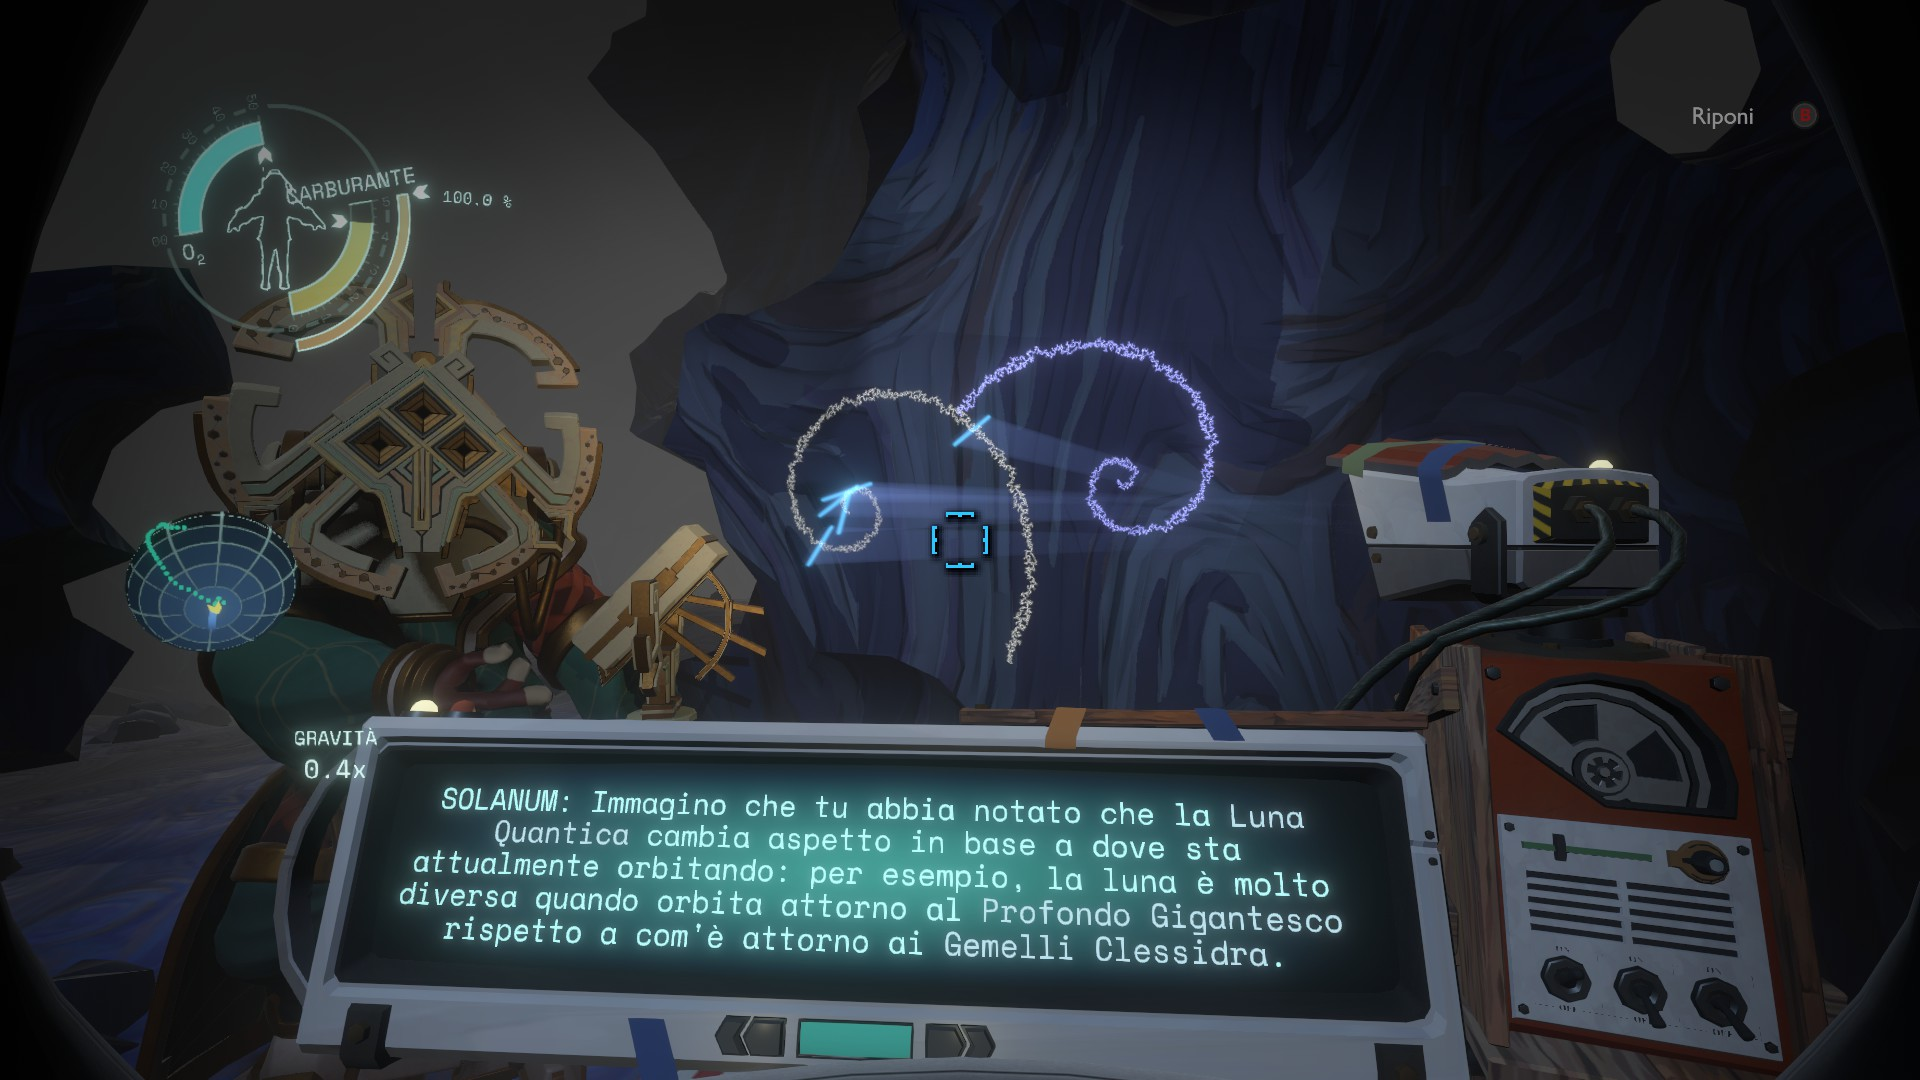
\includegraphics[width=1\textwidth]{Immagini troppo complicate/outer_wilds_1.jpg}
\end{center}
\caption{\scriptsize ``Io e te non sembriamo legare molto. Eppure questo incontro sembra essere speciale. Spero che tu sia d'accordo se ci considero amici.'' -Solanum}\label{fig:img_outer_wilds_1}
\end{figure}






\begin{comment}

Nella prima settimana di settembre 2019 infatti è stato allestito quello che può essere chiamato a tutti gli effetti un "quantum arcade", ovvero una sala giochi quantistica, in un laboratorio congiunto condiviso dall'IBM e dalla \emph{Wits University} di Johannesburg. La sala aveva come scopo quello di mostrare, mediante dei giochi, i principi dell'hardware quantistico a studenti e sviluppatori.

\end{comment}



\chapter{Esplorazione di dungeon mediante Grover} %VIDEOGIOCHI

\begin{comment}
Se il mondo dei videogiochi classici è ancora in fase adolescenziale, considerando che formalmente la loro storia inizia nel 1947 con il \textit{Cathode-ray tube amusement device} e in larga scala nel 1972 con l'avvento di \textit{Pong}\cite{wiki:Storia_dei_videogiochi}, possiamo dire che la loro versione quantistica si trovi ancora in gestazione. Dovremo infatti attendere che la tecnologia quantistica raggiunga un momento di sviluppo avanzato tale da permetterle di arrivare sulle scrivanie delle persone comuni, prima di poter anche solo pensare di usare tale tecnologia per scopi videoludici. Ciò non ci impedisce tuttavia di fantasticare su quali altri risultati potrebbero saltar fuori dal connubio di questi due ambiti. Tra le tante possibilità che potremmo esplorare, una può avere forse maggior rilievo: l'esplorazione di dungeon generati casualmente all'interno di giochi \textit{roguelike}\cite{wiki:Roguelike}. \\
\end{comment}

Nello scorso capitolo abbiamo analizzato una serie di esempi che hanno avuto l'obiettivo comune di avvicinare il mondo del Quantum Computing a quello dei videogiochi. Tuttavia la maggior parte di questi ultimi costruivano alcune delle loro caratteristiche ludiche basandosi su principi della meccanica quantistica, sia per divulgare l'argomento sia per creare esperienze virtuali inedite. Sebbene questo sia ottimo e estremamente efficace in un momento in cui il medium dei videogiochi sta ottenendo sempre più successo e il mondo del Quantum Computing fatica ad essere compreso in modo semplice, pur avendone bisogno per esprimere appieno le proprie potenzialità attraverso le menti e le mani di giovani sviluppatori, esistono anche altri modi di coniugare questi due universi. Ne abbiamo avuto un esempio quando abbiamo parlato di Quantum Pokémon Fight\cite{quantum_pokemon_fight}: l'obiettivo non era quello di ideare nuove meccaniche di gioco, bensì sfruttare i circuiti quantistici per velocizzare operazioni inefficienti o comunque lente. In questo capitolo, seguendo tale filosofia, cercheremo di costruire un circuito che utilizza le potenzialità dell'algoritmo di Grover per l'esplorazione di dungeon generati casualmente all'interno di una particolare categoria di giochi che sta avendo sempre più successo nell'ultimo periodo: i \textit{roguelike}\cite{wiki:Roguelike}. \\
Con il termine \textit{roguelike} (traducibile letteralmente come ``\textit{stile Rogue}'') si intende una categoria di giochi che si ispirano al capostipite del genere: Rogue appunto, videogioco nato nel 1980 sulla base del famoso gioco di ruolo \textit{Dungeons \& Dragons}. L'idea fondamentale era quella di vestire i panni di un esploratore avventuratosi all'interno di un dungeon (labirinto sotterraneo) composto da varie stanze connesse tra di loro mediante corridoi, all'interno delle quali si potevano trovare nemici, potenziamenti o il boss di fine livello. Il gioco originale prevedeva un'interfaccia utente composta da soli caratteri ASCII, ma ad oggi i giochi roguelike sono diventati talmente popolari e di successo da essere sia gradevoli da vedere che da udire, con grafiche e colonne sonore di tutto rispetto. Alcuni elementi comuni di questi giochi, e che anzi li definiscono, sono:
\begin{itemize}
    \item Ad ogni partita il dungeon deve essere generato casualmente, mutando i tipi di stanze, il modo in cui sono connesse e i nemici e potenziamenti che è possibile trovare al loro interno.
    \item Alcuni oggetti all'apparenza identici devono avere effetti diversi in partite diverse. Un'ampolla verde ad esempio potrebbe essere una pozione che potenzia la forza del personaggio in una partita, mentre in quella successiva potrebbe essere un pericoloso veleno.
    \item Quando il personaggio muore, tutti i progressi fatti vengono perduti, e nella partita successiva bisogna ricominciare dal primissimo livello senza alcun tipo di potenziamento. Il senso di progresso in questi giochi viene comunque garantito in modo laterale, ad esempio lo sconfiggere un determinato boss ad un livello avanzato può garantire al giocatore la possibilità di trovare un nuovo tipo di potenziamento nelle sue partite successive.
\end{itemize}
Questa categoria di giochi si distingue nell'avere diversi esponenti che presentano una difficoltà estremamente elevata, richiedendo al giocatore di fallire più e più volte e apprendere dai suoi errori prima di riuscire a concludere una partita. I giocatori più navigati infatti ponderano spesso ogni più piccola decisione, dalle stanze da visitare prima di passare al livello successivo ai potenziamenti da prendere, dato che questi potrebbero avere degli effetti secondari poco gradevoli. Da questo punto di vista si potrebbe pensare al problema dell'esplorazione del dungeon come un problema di ottimizzazione: bisogna attraversare solo alcune stanze prima di combattere il boss e passare oltre, ovvero trovare un giusto \textit{trade-off} tra rischi e guadagni (questa meccanica è meglio nota come \textit{high risk - high reward}), tenendo conto del fatto che alcuni eventi dipenderanno dal caso. Un bravo giocatore è infatti anche uno che sa sfruttare al meglio le risorse che il gioco genera casualmente.
Sarebbe utile quindi avere un agente capace di simulare l'esplorazione del dungeon e dirci quale percorso è meglio imbroccare date le informazioni di cui si dispone, ovvero le proprie statistiche, la stanza corrente e il tipo delle stanze adiacenti. Nell'ambito classico questo può essere visto come un problema di intelligenza artificiale, dove lo scopo è quello di sviluppare un agente che operi in un ambiente parzialmente osservabile e non deterministico. Si tratta quindi di un problema di ricerca che può essere affrontato in due modi: con un approccio \textit{offline} e uno \textit{online}. \\
Nell'approccio \textit{offline} l'agente produrrà un \textit{albero AND-OR} che rappresenta un piano di contingenza, ovvero sequenze alternative di passi tra cui scegliere a seconda degli stimoli che l'ambiente offre. Questo albero presenta due diversi tipi di nodi: nodi OR, in cui la scelta del nodo figlio dipende esclusivamente dall'agente, e nodi AND, dove invece la scelta del successore dipende dal caso, cioè dalle contingenze dell'ambiente. Ogni percorso che va dal nodo radice a un nodo foglia è una possibile sequenza di eventi a cui può andare incontro l'agente quando deve esplorare l'ambiente circostante. Una volta che tutti i nodi foglia sono stati determinati l'agente sarà sempre in grado di effettuare ``la scelta giusta''. Il problema principale (comunque affrontato da varianti di questo approccio offline) sta nel fatto che talvolta possono crearsi cammini lungo l'albero di profondità infinita, formando di fatto dei loop. Legato a ciò vi è inoltre un secondo problema, tipico dell'intelligenza artificiale: la quantità di memoria richiesta per mantenere un albero che potenzialmente può avere profondità infinita. \\
L'approccio \textit{online}, di contro, preferisce alternare computazione e azione, soprattutto quando l'ambiente è non deterministico, consentendo "\textit{all'agente di concentrare le attività di calcolo sulle contingenze che si verificano effettivamente, anziché su quelle che potrebbero verificarsi ma probabilmente non lo faranno}"(per maggiori informazioni si veda il Capitolo 4.5 di \cite{aima}). Questo tipo di approccio può essere preferibile nell'ambito dell'esplorazione di un dungeon ignoto, poiché gli effetti di alcune azioni potrebbero essere sconosciuti all'agente fino a che tali azioni non siano state messe in atto (un giocatore non può sapere se prenderà danno o meno entrando in una specifica stanza: deve entrarci per scoprirlo). \\
Seguendo quest'ultimo approccio abbiamo deciso di sviluppare un algoritmo di ricerca online per l'esplorazione di un dungeon generato casualmente. Tale dungeon presenta una serie di semplificazioni, rispetto a un caso reale, dovute sia al fatto che vuole essere rappresentativo dei roguelike in generale, sia al fatto che dati i limiti della teconlogia quantistica odierna non è possibile lavorare efficientemente con troppi qubit. Presenteremo dunque due esempi di esplorazione, da parte di un agente, di un dungeon non deterministico e parzialmente osservabile, dove utilizzeremo l'algoritmo di Grover per scegliere lo stato successivo migliore tra quelli disponibili.
\begin{itemize}
    \item Nel primo esempio il nostro agente dovrà esplorare un dungeon composto soltanto da quattro stanze, dove l'algoritmo di Grover opererà su un solo qubit. Pur essendo un caso di applicazione in cui l'algoritmo non è in grado di mostrare il suo vero potenziale, lo tratteremo ugualmente per prendere familiarità con le semplificazioni utilizzate anche nel caso successivo.
    \item Nel secondo esempio complicheremo la struttura del dungeon portando il numero di stanze da quattro a otto e aggiungendone una nuova tipologia. Introdurremo inoltre delle statistiche (salute e attacco) di cui l'agente dovrà tenere di conto al momento della scelta dell'azione successiva.
\end{itemize}

\section{Esplorazione (quantistica) di un dungeon a quattro stanze}
In questo esempio il nostro agente si troverà a doversi muovere all'interno di un dungeon composto da quattro stanze. Ad ogni stanza è assegnato un indice univoco a due bit, e ciascuna di queste è connessa, mediante dei corridoi, ad altre due stanze, in particolare quelle il cui indice è ottenuto effettuando lo swap di un solo bit dell'indice corrente (ad esempio la stanza 00 sarà connessa alle stanze 01 e 10). Possiamo quindi vedere il labirinto come un grafo non orientato e senza pesi sugli archi, poiché il movimento da una stanza all'altra ha sempre costo costante e comunque non ci interessa. Ciascuna stanza può contenere uno di questi tre elementi al suo interno:
\begin{enumerate}
    \item Dei nemici
    \item Un tesoro
    \item Il boss del dungeon
\end{enumerate}
All'avvio di ogni partita ad ogni stanza viene assegnato un contenuto casuale, con alcuni vincoli:
\begin{itemize}
    \item La stanza 00, che sarà sempre la prima stanza da esplorare nel labirinto, può contenere solamente dei nemici.
    \item Il resto del labirinto (ovvero le altre tre stanze) deve essere sempre composto da esattamente una stanza contenente il tesoro, una contenente il boss e una popolata da nemici. L'associazione \textit{indice-contenuto} di queste stanze è generata casualmente all'inizio di una partita.
    \item L'effetto di una stanza si attiva nel momento in cui l'agente vi entra. A questo livello di semplificazione è difficile vedere gli effetti di questa regola, ma l'idea è che se ad esempio il nostro protagonista entra in una stanza piena di nemici, vi combatte, e se sopravvive può fermarsi un attimo per riposare e ponderare dove sia meglio spostarsi adesso.
    \item Quando l'agente esce dalla stanza del tesoro (ovvero dopo aver ottenuto il potenziamento ivi contenuto) questa viene popolata immediatamente da nemici. % Questo meccanismo è necessario affinché l'agente non pensi di poter mettere piede più e più volte in questa stanza sperando di trovare innumerevoli tesori. 
    Il motivo per cui la riempiamo di nemici e non la lasciamo vuota è sempre legato alla nostra semplificazione, ma serve anche a disincentivare l'agente dal percorrere stanze già visitate in favore dell'ignoto.
\end{itemize}
Con questa definizione del problema lo scopo del nostro agente è molto semplice: una volta entrato nel dungeon questi deve trovare la stanza del tesoro, per poi dirigersi verso il boss. In tutto questo deve visitare meno stanze contenenti nemici possibile. Come ogni agente che si rispetti, questi avrà delle percezioni, in particolare saprà sempre il contenuto delle stanze adiacenti a lui (non ha bisogno di sapere gli indici di queste stanze in quanto, questi, sono dati implicitamente dall'indice della stanza corrente, che invece l'agente conosce). La funzione di transizione per il nostro avventuriero, che corrisponde al nostro oracolo nell'algoritmo di Grover, è quindi molto semplice, e può essere schematizzata nel seguente pseudocodice:
\begin{algorithm}[H]
\begin{algorithmic}[1]
\Procedure{quantum\_choice}{$current\_room, treasure\_seen, adjacent\_rooms$}
    \If{$adjacent\_rooms.contains(treasure\_room)$}
        \Let{$current\_room$}{$treasure\_room$}
        \Let{$treasure\_seen$}{$True$}
    \ElsIf{\textbf{not} $treasure\_seen$ \textbf{and} $adjacent\_rooms = [enemies, boss]$}
        \Let{$current\_room$}{$enemies$}
    \ElsIf{$treasure\_seen$ \textbf{and} $adjacent\_rooms = [enemies, enemies]$}
        \Let{$current\_room$}{$adjacent\_rooms.chooseRandom()$}
    \ElsIf{$treasure\_seen$ \textbf{and} $adjacent\_rooms.contains(boss)$}
        \Let{$current\_room$}{$boss$}
    \EndIf
\EndProcedure
\end{algorithmic}
\end{algorithm}

% \begin{enumerate}
%     \item Se non ha ancora visto il tesoro e una delle stanze adiacenti lo contiene, si sposta in essa.
%     \item Se non ha ancora visto il tesoro e ha adiacenti la stanza del boss e una con nemici, si sposta in quest'ultima. Infatti l'agente non può andare dal boss finché non ha trovato il tesoro.
%     \item Se ha preso il tesoro e ha adiacenti solo stanze con nemici, ne sceglie casualmente una. In questo esempio così semplice infatti basta enumerare tutti i possibili dungeon che possono venire a crearsi per rendersi conto che, al prossimo passo, il boss sarà sicuramente adiacente.
%     \item Se ha preso il tesoro e ha il boss adiacente a te, va da quest'ultimo.
% \end{enumerate}

Per implementare dunque l'esplorazione online del nostro agente nel labirinto possono bastarci 7 qubit: 
\begin{itemize}
    \item Un qubit $\ket{\psi}$ posto nello stato di ugual sovrapposizione a cui dovrà essere applicato il kickback di fase -1 quando si è deciso che direzione prendere. In particolare a seconda dello stato che verrà misurato da questo qubit si sceglierà se andare nella stanza a sinistra (ovvero quella ottenuta effettuando lo swap del primo bit di indice della stanza corrente) o a destra (swappando invece il secondo bit).
    \item Due qubit che descrivano il contenuto della stanza a sinistra (data un'associazione arbitraria, per esempio 00 = tesoro, 01 = nemico e 11 = boss).
    \item Due qubit che descrivano il contenuto della stanza a destra.
    \item Un qubit che indichi se si è già esplorata la stanza del tesoro.
    \item Un qubit, quello dell'oracolo, inizializzato nello stato $\ket{-}$ che applichi il kickback di fase al qubit $\ket{\psi}$ quando necessario.
\end{itemize}
Ci serve poi, oltre a questi qubit, un bit classico per conservare il risultato della misura del qubit $\ket{\psi}$. A questo punto possiamo eseguire l'intero algoritmo di Grover più e più volte utilizzando l'output di una fase per quella successiva, fino a quando l'agente non rileva di essere giunto al boss. L'intero codice scritto in Qiskit che implementa questo algoritmo di esplorazione è riportato nell'appendice A. Mostriamo qua solamente un'immagine del circuito ottenuto durante una delle esecuzioni dell'algoritmo di Grover. Diciamo ``una delle esecuzioni'' in quanto, essendo l'output di ogni circuito l'input del successivo, può essere necessario modificare alcune porte di ingresso tra una stanza esplorata e l'altra. Infatti una volta misurato il bit classico ed esplorata la stanza successiva cambieranno l'indice della stanza corrente, i contenuti delle stanze adiacenti e forse avremo trovato il tesoro. Nella successiva esecuzione del circuito bisognerà tenere di conto di questi fatti, applicando porte NOT ai qubit che li descrivono laddove necessario.

\begin{figure}[H]
\captionsetup{font=scriptsize}
\begin{center}
    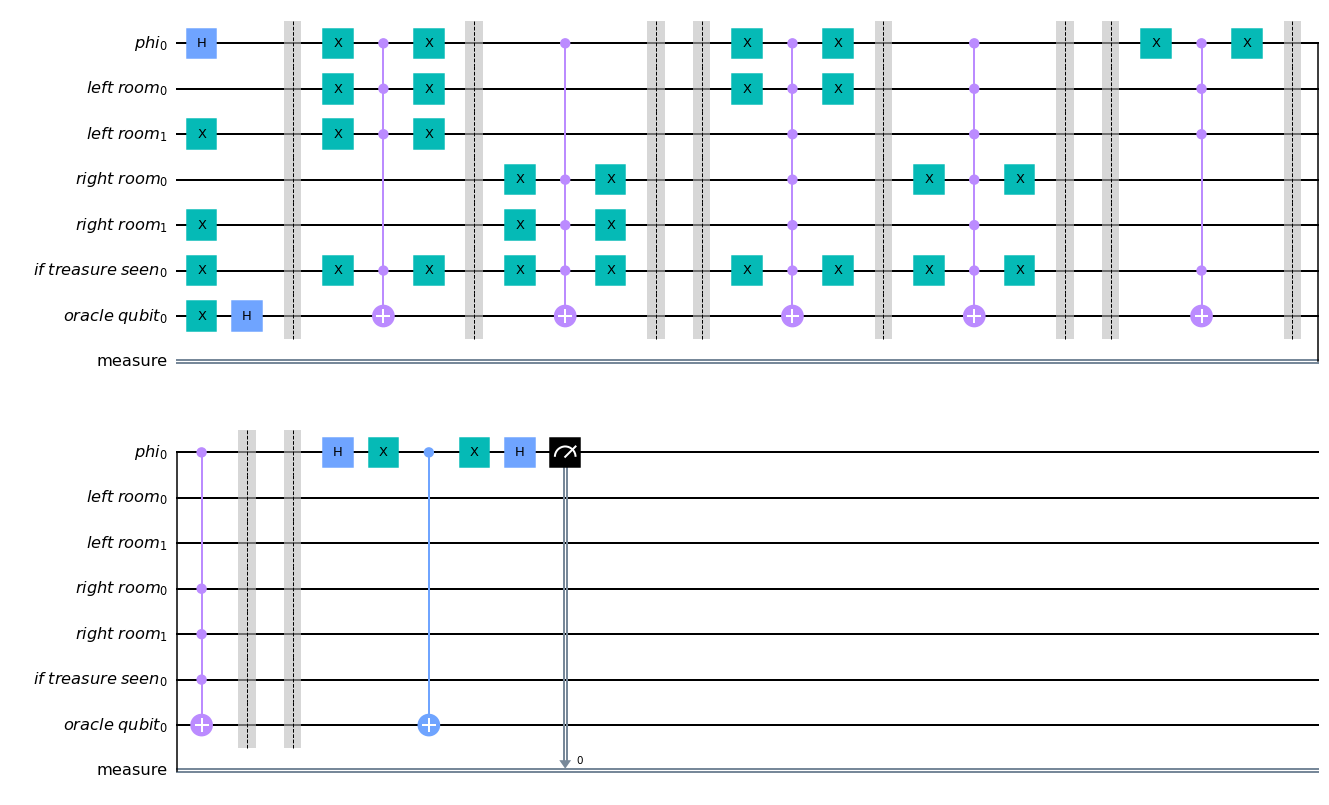
\includegraphics[width=16cm]{Immagini troppo complicate/2x2_labyrinth_first_circuit.png}
\end{center}
\caption{\scriptsize Esempio di circuito ottenuto per la scelta della stanza successiva in un labirinto a quattro stanze.}\label{fig:circ_2x2}
\end{figure}
\noindent Come anticipato questo esempio ha solo uno scopo illustrativo e preparatorio a quello che segue, in quanto qui l'uso dell'algoritmo di Grover non è necessario per effettuare la scelta: anzi, è completamente inutile, dato che, lavorando noi su un solo qubit per scegliere che direzione prendere, finiamo col riflettere semplicemente il vettore $\ket{\psi}$ rispetto a $\ket{\beta}$ (applichiamo l'operatore di Grover una sola volta), non migliorando minimamente la situazione e avendo sempre la stessa probabilità di misurare 0 o 1 (ricordiamo inoltre che $\ket{\beta}$ era il vettore di ugual sovrapposizione dei successi, dove giacciono le soluzioni). L'esecuzione relativa a questo esempio riportata nell'appendice A infatti è un caso fortunato in cui l'agente ha scelto un percorso ottimale, data la mappa iniziale. Vediamo ora di complicare leggermente le cose così da renderle più interessanti, sia dal punto di vista della formulazione del problema, sia da quello dell'utilizzo di Grover.

\section{Esplorazione di un dungeon a otto stanze}
\subsection{Implementazione classica}

Per rendere le cose più interessanti, oltre all'ampliamento del dungeon, introduciamo le statistiche di salute e di attacco, che l'agente dovrà considerare al momento della scelta della stanza successiva. Anche in questo caso ogni stanza è identificata univocamente da un indice a tre bit, che implicitamente indica anche le tre stanze adiacenti raggiungibili. Le regole fondamentali del gioco sono le stesse di prima, con qualche nota aggiuntiva:
\begin{itemize}
    \item L'agente, che comincerà sempre la sua esplorazione dalla stanza di indice 000, partirà avendo quattro punti salute, il massimo possibile. Sarà importante mantenere il valore di questa statistica strettamente sopra lo zero, sia per evitare di essere uccisi dai nemici, sia per aumentare le chance di battere il boss.
    \item Anche la statistica di attacco gioca un ruolo fondamentale. Tanto più è alta, tanto più diviene facile evitare di essere colpiti dai nemici, e tanto più sarà facile sconfiggere il boss. Inizialmente il nostro agente sarà molto debole e avrà solo un punto attacco, ma potrà migliorare questa statistica sia visitando il tesoro che il negozio.
\end{itemize}
Approfondiamo maggiormente queste ultime due stanze.\\
Il tesoro, che prima fungeva semplicemente da stanza necessaria a rendere il problema dell'esplorazione appena più complicato, qui gioca un ruolo fondamentale. Entrandoci, l'agente potrà trovare una qualunque tra queste quattro ricompense:
\begin{itemize}
    \item Un punto salute.
    \item Due punti salute.
    \item Un punto attacco.
    \item Due punti attacco.
\end{itemize}
Se i punti attacco garantiscono sempre un potenziamento netto all'esploratore, dall'altro esistono situazioni in cui quelli salute risultano completamente inefficaci. Ad esempio, se l'agente entra nella stanza del tesoro con tre punti salute e trova due punti salute, potrà ottenerne solo uno.\\
Il negozio invece, se visitato, sottrae un punto salute all'agente, ma ne aggiunge uno di attacco. Questo scambio risulterà essere a volte vantaggioso, a volte indifferente e a volte persino dannoso: dipende da ciò che l'agente ha già visto, dal valore corrente delle sue statistiche e dalla configurazione del dungeon.\\
Ma perché crucciarsi tanto per tenere alte queste statistiche? Per due motivi, fondamentalmente. Il primo è che, entrando in una stanza piena di nemici, si può venire danneggiati, e ciò comporta la perdita di un punto salute. Se questi scendono a zero, si muore, e l'esplorazione termina con un fallimento. Se da un lato quindi l'idea di potersi curare trovando punti salute nella stanza del tesoro sembra una prospettiva niente male, dall'altro è comunque una buona notizia (se non addirittura migliore) trovare dei punti attacco, dato che questi modificano le probabilità di essere colpiti dai nemici in una stanza che li contiene. In particolare, si ha che, entrando in una stanza contenente nemici avendo:
\begin{itemize}
    \item un solo punto attacco, si ha il 75\% di probabilità di essere danneggiati.
    \item due punti attacco, si ha il 50\% di probabilità di essere danneggiati.
    \item tre punti attacco, si ha il 25\% di probabilità di essere danneggiati.
    \item quattro punti attacco, non si verrà danneggiati.
\end{itemize}
Le statistiche di salute e attacco sono però fondamentali soprattutto per il fatto che determinano la percentuale di vittoria sul boss una volta raggiunto, seguendo la Tabella \ref{table:6.1}.
\begin{table}[H]
\captionsetup{font=scriptsize}
\centering
\begin{tabular}{|c|c|c|c|c|}
    \hline
      & attacco = 1 & attacco = 2 & attacco = 3 & attacco = 4\\
         \hline
    salute = 1 & 10\% & 20\% & 30\% & 40\%\\
         \hline
    salute = 2 & 15\% & 30\% & 45\% & 60\%\\   
         \hline
    salute = 3 & 20\% & 40\% & 60\% & 80\%\\     
         \hline
    salute = 4 & 25\% & 50\% & 75\% & 100\%\\
        \hline
\end{tabular}
\caption{\scriptsize Percentuali di vittoria contro il boss sulla base dei punti salute e attacco.}\label{table:6.1}
\end{table}
\noindent È possibile definire questa percentuale in forma più compatta mediante l'equazione:
\begin{figure}[H]
\begin{displaymath}
\text{probabilità di vittoria} = 5 \times (1 + \text{salute}) \times \text{attacco.}
\end{displaymath}
\end{figure}
\noindent Anche in questo caso ci sono alcuni vincoli sulla struttura del dungeon (sempre generato casualmente) che seguono logicamente da quelli già visti nel caso delle quattro stanze, con qualche aggiunta:
\begin{itemize}
    \item La stanza 000 sarà sempre quella iniziale, e potrà contenere solo nemici.
    \item Il resto del labirinto si compone di esattamente:
    \begin{itemize}
        \item Una stanza del tesoro.
        \item Un negozio.
        \item Una stanza del boss.
        \item Quattro stanze contenenti nemici.
    \end{itemize}
    \item Quando l'agente entra in una stanza, se ne attiva l'effetto, ovvero:
    \begin{itemize}
        \item Entrando in una stanza popolata da nemici viene deciso in modo stocastico se l'agente ha preso danno (cioè ha perso un punto salute) o meno, sulla base dei suoi punti attacco e salute.
        \item Entrando nella stanza del tesoro viene scelto casualmente un potenziamento e applicato alle statistiche, se possibile.
        \item Entrando nel negozio viene automaticamente sottratto un punto salute all'agente, che in cambio riceve un punto attacco aggiuntivo.
    \end{itemize} 
    \item L'agente non può avere più di quattro punti per statistica. Per come stiamo formulando il problema del dungeon a otto stanze non c'è pericolo che si possano ottenere più di quattro punti attacco, ma lo stesso non può essere detto per la salute. Se ad esempio l'agente entrasse nella stanza del tesoro con tutti e quattro i punti salute e trovasse come potenziamento uno o due punti di questa statistica, non potrebbe ottenerli, e tale potenziamento andrebbe perso per la partita corrente.
    \item Nel caso della stanza del tesoro e del negozio, subito dopo che l'agente vi è entrato e i loro effetti sono stati applicati, queste si trasformano in stanze contenenti nemici. Ciò non implica che l'agente debba subito combattere con loro, in quanto abbiamo detto che l'effetto di una stanza si applica solo al momento dell'entrata. Se tuttavia, per qualche motivo, l'agente dovesse tornare in queste stanze in futuro, non solo non troverà alcun tipo di potenziamento, ma dovrà scontrarsi con dei nemici.
    \item L'esplorazione dell'agente può terminare prematuramente se, entrando in una stanza contenente nemici, i suoi punti salute scendono a zero.
    \item Quando l'agente entra nella stanza del boss viene deciso, sempre casualmente e in accordo con le probabilità riportate nella Tabella \ref{table:6.1}, se questi è riuscito a vincere contro il boss oppure ha perso, facendosi uccidere da esso. 
\end{itemize}
L'esplorazione che il nostro protagonista deve condurre questa volta non è banale. Sicuramente dovrà visitare il tesoro, dato che nel migliore dei casi aumenterà una delle sue statistiche e nel peggiore rimarrà com'era prima. Il negozio, d'altra parte, non è sempre una tappa obbligatoria. Togliendo un punto salute e aggiungendo un punto attacco, a volte può migliorare significativamente la probabilità di vittoria, a volte può lasciarla inalterata e a volte può addirittura peggiorarla. Basta confrontare ogni cella della tabella \ref{table:6.1} con quella che le sta in alto a destra (rappresentativa della probabilità di sconfiggere il boss con un punto salute in meno e uno di attacco in più) per vedere se vale la pena entrare in questa stanza. È chiaro dunque che l'avventuriero dovrà cambiare la propria strategia esplorativa sulla base delle statistiche correnti, delle stanze adiacenti e degli effetti che queste avrebbero su di esso se ci entrasse, tenendo di conto anche alcune stanze già esplorate. Ragionando dunque sulle varie situazioni in cui questi può trovarsi, abbiamo scritto un programma Python che implementa l'esplorazione dell'agente all'interno del dungeon, con una funzione di transizione che assegna un valore numerico ad ogni stanza adiacente a seconda di vari fattori. Dopo questo assegnamento, viene selezionata la stanza di valore massimo, e l'esplorazione procede in essa. L'agente conoscerà sempre i suoi punti salute, punti attacco, la stanza corrente, il contenuto delle stanze adiacenti, se ha già visitato la stanza del tesoro e se ha già visto il negozio, tutti fattori determinanti per la decisione di quale sia la prossima stanza in cui mettere piede. I valori riportati nel codice, apparentemente casuali, sono stati scelti in seguito a ragionamenti sulla struttura del problema e prove ripetute, dimostrandosi adatti ai nostri scopi su un numero di esecuzioni che supera le centinaia di migliaia. Riportiamo in pseudocodice la funzione di transizione (l'intero codice sorgente è disponibile nell'appendice):

\begin{algorithm}[H]
\begin{algorithmic}[1]
\Procedure{chance\_victory}{$health, attack$}
    \State \Return{$5 \times (1 + health) \times attack$}
\EndProcedure
\Procedure{classical\_choice}{$current, treasure\_explored, shop\_seen, adjacents, health, attack$}
\Let{$S$}{$health$}
\Let{$A$}{$attack$}
\If{$current = tresure\_room$}
    \Let{$treasure\_explored$}{$True$}
\EndIf
\If{$current = shop\_room$}
    \Let{$shop\_seen$}{$True$}
\EndIf
\For {$room$ \textbf{in} $adjacents$}
    \If{$room = treasure$ \textbf{and not} $treasure\_explored$}
        \Let{$room.value$}{10}
    \EndIf
    \If{$room = shop$ \textbf{and} $health = 1$}
        \Let{$room.value$}{-1}
    \EndIf
    \If{$room = shop$ \textbf{and} $chance\_victory(S-1, A+1) > chance\_victory(S, A)$}
        \Let{$room.value$}{8}
    \EndIf
    \If{$room = shop$ \textbf{and} $chance\_victory(S-1, A+1) = chance\_victory(S, A)$}
        \Let{$room.value$}{6}
    \EndIf
    \If{$room = shop$ \textbf{and} $chance\_victory(S-1, A+1) < chance\_victory(S, A)$}
        \Let{$room.value$}{0}
    \EndIf
    \If{$room = boss$ \textbf{and not} $treasure\_explored$}
        \Let{$room.value$}{0}
    \EndIf
    \If{$room = boss$ \textbf{and} $treasure\_explored$ \textbf{and} $shop\_seen$}
        \Let{$room.value$}{7}
    \EndIf
    \If{$room = boss$ \textbf{and} $treasure\_explored$ \textbf{and not} $shop\_seen$ \textbf{and} \par
        \hskip\algorithmicindent $(S = 1$ \textbf{or} $chance\_victory(S-1, A+1) < chance\_victory(S, A))$}
        \Let{$room.value$}{3}
    \EndIf
    \If{$room = boss$ \textbf{and} $treasure\_explored$ \textbf{and not} $shop\_seen$ \textbf{and} \par
        \hskip\algorithmicindent $chance\_victory(S-1, A+1) > chance\_victory(S, A)$}
        \Let{$room.value$}{1}
    \EndIf
    \If{$room = enemies$}
        \Let{$room.value$}{2}
    \EndIf
\EndFor
\If{$adjacents.contains(shop)$}
    \Let{$shop\_seen$}{$True$}
\EndIf
\Let{$current$}{$max\_value(adjacents)$}
\EndProcedure
\end{algorithmic}
\end{algorithm}

%In particolare, data una qualunque stanza adiacente a quella corrente, le viene assegnato uno %tra i seguenti valori se vengono soddisfatti i criteri relativi:
% \begin{itemize}
%     \item 10: se la stanza contiene il tesoro e ancora non lo si è esplorato.
%     \item -1: se la stanza contiene il negozio ma si ha un solo punto salute.
%     \item 8: se la stanza contiene il negozio e entrandoci le chance di vittoria aumentano.
%     \item 6: se la stanza contiene il negozio e entrandoci le chance di vittoria non cambiano.
%     \item 0: se la stanza contiene il negozio e entrandoci le chance di vittoria diminuiscono, oppure se la stanza contiene il boss e non è ancora stato trovato il tesoro.
%     \item 7: se la stanza contiene il boss, è stata esplorata la stanza del tesoro e si è visto il negozio.
%     \item 3: se la stanza contiene il boss, si è già esplorata la stanza del tesoro, non si è visto il negozio e non ha senso cercarlo (perché si ha un punto vita o perché anche andandoci le chance di vittoria non aumenterebbero).
%     \item 1: se la stanza contiene il boss, si è già esplorata la stanza del tesoro, non si è visto il negozio e lo si vuole cercare perché aumenterebbe le chance di vittoria.
%     \item 2: se la stanza contiene nemici.
% \end{itemize}
% In alcune situazioni l'agente dovrà anche aggiornare le sue variabili che indicano se ha esplorato la stanza del tesoro e visto il negozio:
% \begin{itemize}
%     \item Se l'agente ha appena esplorato la stanza del tesoro, se lo segna.
%     \item Se l'agente ha appena esplorato il negozio, si segna di averlo visto.
%     \item Se l'agente ha già esplorato la stanza del tesoro e si trova adiacente il negozio, si segna di averlo visto, indipendentemente dal fatto che poi ci entri o meno. Basta ragionare un attimo su quello che può fare l'agente una volta esplorato il tesoro per capire il perché di questa scelta implementativa: se entrando nel negozio la probabilità di vittoria aumenta, è certo che l'agente favorirà questa stanza rispetto ad una contenente nemici o a quella in cui dimora il boss. Se però questo non succede, tanto vale andare direttamente dal boss, perché tanto, avendo già esplorato la stanza del tesoro, non si hanno chance di aumentare i punti salute, che potrebbero ridare importanza al negozio. È per questo che abbiamo distinto il concetto di ``esplorare'' una stanza da quello di ``vederla''. L'agente vorrà sempre esplorare la stanza del tesoro, mentre a volte potrebbe aver visto il negozio senza averlo esplorato.
% \end{itemize}
\subsection{Implementazione quantistica}

Per l'implementazione quantistica il ragionamento è analogo, e il codice rimane identico salvo per la parte in cui l'agente deve scegliere la stanza successiva. La funzione di transizione è infatti rappresentata da un circuito quantistico che implementa l'algoritmo di Grover per la scelta della prossima stanza. La differenza fondamentale è che, se prima si assegnava un valore numerico a ogni stanza adiacente e poi si prendeva quella che lo massimizzava, qui l'obiettivo dell'algoritmo di Grover è, date le informazioni correnti dell'agente, determinare quale dei tre bit che descrivono l'indice della stanza corrente è meglio invertire, così da ottenere l'indice della migliore stanza successiva. La scelta della prossima stanza si può riassumere nel seguente pseudocodice:
%Per fare ciò si inizializza un registro da due qubit nello stato di ugual sovrapposizione $\ket{\phi}$, applicando poi l'oracolo e il diffusore esattamente una volta. Il risultato della misurazione di questo registro ci dirà in quale stanza l'agente continuerà la sua esplorazione, posta a priori una semantica che associa ai due qubit misurati un bit della stanza corrente da flippare (nel nostro codice: 00 = flip del primo bit, 01 = flip del secondo bit, 10 = flip del terzo bit.

\begin{algorithm}[h]
\begin{algorithmic}[1]
\Procedure{quantum\_choice}{$current\_room, \ket{\phi}, work\_qubits$}
    \Let{$new\_room\_chosen$}{$False$}
    \While{\textbf{not} $new\_room\_chosen$}
        \Let{$circuit$}{$new\_quantum\_circuit(current\_room, \ket{\phi}, work\_qubits)$}
        \State $grover\_oracle(circuit)$
        \State $diffuser(circuit)$
        \Let{$result$}{$execute(circuit)$}
        \Let{$direction$}{$measure\_\ket{\phi}(result)$}
        \If{$direction = 00$}
            \Let{$tmp$}{$current\_room.flip\_index(0)$} \algorithmiccomment{stanza a sinistra}
        \EndIf
        \If{$direction = 01$}
            \Let{$tmp$}{$current\_room.flip\_index(1)$} \algorithmiccomment{stanza al centro}
        \EndIf
        \If{$direction = 10$}
            \Let{$tmp$}{$current\_room.flip\_index(2)$} \algorithmiccomment{stanza a destra}
        \EndIf
         \If{$direction = 00$ \textbf{or} $direction = 01$ \textbf{or} $direction = 10$}
            \Let{$new\_room\_chosen$}{$True$}
            \Let{$current\_room$}{$tmp$}
        \EndIf
    \EndWhile
\EndProcedure
\end{algorithmic}
\end{algorithm}

\newpage

\begin{figure}[H]
\captionsetup{font=scriptsize}
\begin{center}
    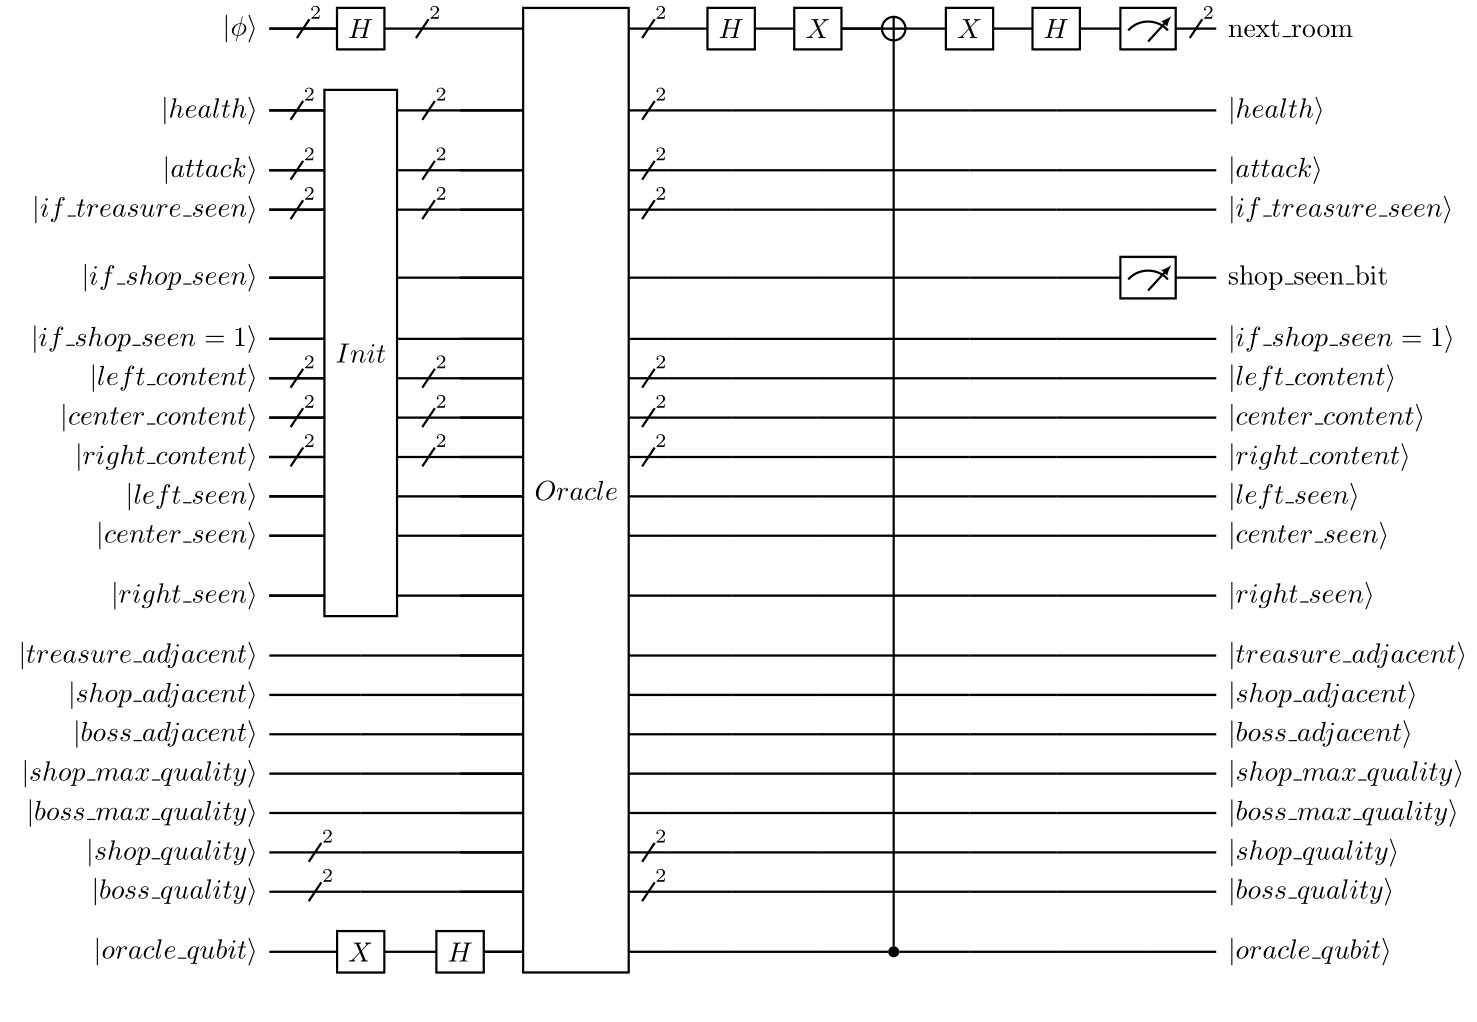
\includegraphics[width=1\textwidth]{Immagini troppo complicate/circuito_8_stanze_2.png}
\end{center}
\caption{\scriptsize Esempio di circuito ottenuto per la scelta della stanza successiva in un labirinto a otto stanze}\label{fig:circ_2^3}
\end{figure}
\noindent Per come abbiamo costruito il circuito, lo spazio di ricerca (ovvero le tre stanze adiacenti) conterrà sempre al più una sola soluzione. Dato che però stiamo usando due qubit ($\ket{\phi}$) per la ricerca, può accadere, raramente, che venga misurato 11, e in tal caso si chiede all'agente di ripetere la scelta. Potrebbe di fatto non esserci una stanza preferita, e in tal caso la misura dei due qubit nello stato $\ket{\phi}$ restituirà un valore casuale, che corrisponde al comportamento che ci aspettiamo dall'agente in caso di mancanza di una preferenza. Proprio perché lo spazio di ricerca conterrà sempre al massimo una soluzione, il numero di rotazioni da eseguire, e quindi di applicazioni dell'operatore di Grover, è al più uno, come già visto nel Capitolo 2. Potevamo anche aggiungere un terzo qubit al registro $\ket{\phi}$ così da applicare sempre l'operatore di Grover il numero di volte necessario, sapendo a priori che cinque delle otto possibili soluzioni sarebbero state sbagliate. Tuttavia, dato che il circuito costruito si compone già di ventotto qubit, non abbiamo ritenuto saggio introdurne un altro, considerando che ciò avrebbe potuto anche portare all'aggiunta di ulteriori qubit di lavoro. Infatti, a seconda della stanza corrente, di quelle adiacenti e dello stato dell'agente, il numero di soluzioni può variare, e ciò implica maggiore logica per il circuito. Abbiamo preferito costruirne uno \textit{ad hoc} che sfruttasse a pieno i qubit disponibili, riciclandoli quando necessario. A scanso di equivoci, specifichiamo quindi che il circuito così costruito può essere personalizzato nella scelta dei contenuti delle varie stanze, \textbf{nel rispetto dei vincoli del problema citati sopra}: in particolare, la prima stanza (di indice 000) dovrà sempre contenere nemici ed essere il punto di ingresso per il dungeon, ci dovrà essere sempre esattamente un tesoro, un negozio, un boss, e altre quattro stanze contenenti nemici.
\begin{figure}[H]
\captionsetup{font=scriptsize}
\begin{center}
    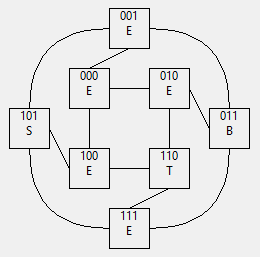
\includegraphics[width=5cm]{Immagini troppo complicate/Dungeon_usato.png}
\end{center}
\caption{\scriptsize Esempio di dungeon a otto stanze che rispetta i vincoli del problema. Ogni lettera rappresenta il maniera sintetica il contenuto della stanza, dove S = Shop, E = Enemies, T = Treasure e B = Boss.}\label{fig:img_dungeon_example}
\end{figure}
\noindent Come però si decide di mappare questo insieme di stanze agli otto indici di stanza, è a nostra discrezione, e il circuito quantistico (così come il codice classico) fornirà sempre il percorso che ha la maggiore probabilità di far vincere l'agente. Non entreremo ulteriormente nei dettagli implementativi del circuito, limitandoci a confrontarlo con la sua versione classica e fare un'analisi costi-benefici di queste due implementazioni. Anche in questo caso, per il lettore interessato, il codice sorgente del circuito scritto in Qiskit è disponibile nell'appendice C, adeguatamente commentato così da permettere a chiunque di seguire passo passo il ragionamento dietro la sua costruzione. Ci teniamo inoltre a specificare che l'algoritmo quantistico permette solo di velocizzare il passo di scelta, e non influisce in alcun modo sulla probabilità di vittoria dell'agente. A riprova di ciò riportiamo l'esito dell'esplorazione del medesimo dungeon, effettuata sia col codice classico che con quello quantistico, nella Figura 4.4.\\
\begin{figure}[H]
    \captionsetup{font=scriptsize}
    \centering
    \subfloat[\scriptsize Esito dell'algoritmo classico su 100 esecuzioni]{{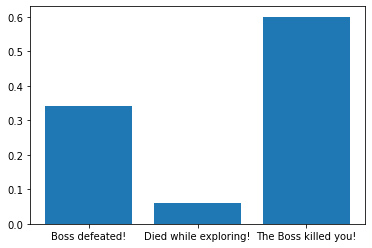
\includegraphics[width=7cm]{Immagini troppo complicate/Classic_histogram.png} }}
    \qquad
    \subfloat[\scriptsize Esito dell'algoritmo quantistico su 100 esecuzioni]{{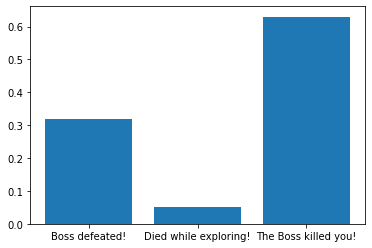
\includegraphics[width=7cm]{Immagini troppo complicate/Quantum_histogram.png} }}
    \caption{\scriptsize Confronto delle esecuzioni classiche con quelle quantistiche. L'algoritmo di esplorazione classico e quello quantistico sono stati eseguiti partendo dallo stesso dungeon (in particolare quello della Figura \ref{fig:img_dungeon_example}), e per entrambi sono state effettuate 100 esecuzioni (esplorazioni). I risultati sono molto simili, come ci aspettavamo, in quanto la strategia di esplorazione è sempre la stessa.}\label{fig:histogram_comparison}
\end{figure}
\noindent La complessità dell'algoritmo di esplorazione risiede nella scelta della prossima stanza in cui mettere piede e nel numero di volte che questa operazione viene effettuata. Per poter decidere infatti lo stato successivo l'algoritmo classico deve prima invocare la funzione \textit{assign\_quality()} su ogni stanza adiacente, che assegna a ciascuna di queste un valore qualitativo dipendente da fattori come la salute, l'attacco, le stanze precedentemente esplorate e via discorrendo. Dopo di che va trovato il massimo tra questi valori, così da ottenere la stanza vincitrice di questo processo di scelta. Indipendentemente dalla struttura dati utilizzata per conservare i valori delle stanze, nel caso peggiore la ricerca del massimo avrà complessità $\mathcal{O}(N)$, se immaginiamo che ogni stanza ne abbia $N$ adiacenti. Con un circuito quantistico che implementa la funzione di transizione, tuttavia, la complessità scende a $\mathcal{O}(\sqrt{N})$ (a patto che l'operatore di Grover sia stato scritto correttamente). Su esempi piccoli come quelli esaminati fino ad ora il vantaggio quantistico non solo non lo si vede, ma non lo si ha nemmeno, data la pochezza di computer quantistici capaci di gestire un numero così elevato di qubit e del rumore quantistico. Infatti tutte le simulazioni su Qiskit del labirinto ad otto stanze sono state eseguite su un computer classico che ne simula uno quantistico. Tuttavia, augurandoci che negli anni a venire questa tecnologia riesca a permetterci di gestire il rumore, costruire computer quantistici a molti qubit, fare arrivare questi nelle nostre case e, chissà, permetterci di avere un linguaggio di programmazione di più alto livello per costruire programmi quantistici, il miglioramento della performance si paleserebbe nel caso di labirinti molto grandi.\\
\subsection{Possibili generalizzazioni}
Fino ad ora abbiamo presentato programmi quantistici atti all'esplorazione di labirinti a quattro e otto stanze. Ma se volessimo gestire dimensioni arbitrarie per il dungeon, saremmo capaci di farlo?\\
Ebbene, quando abbiamo raddoppiato la dimensione del labirinto, abbiamo anche modificato la formulazione del problema, introducendo nuove statistiche, stanze e variabili, e ciò ha comportato una completa rivisitazione del circuito. È chiaro che, se volessimo procedere per questa strada introducendo cose come punti difesa, mini-boss e caratteristiche simili, dovremmo ancora una volta mettere mano ai qubit e alle porte. D'altro canto, semplici modifiche alla dimensione del dungeon non richiederebbero cambiamenti troppo drastici. Fintanto che il nostro labirinto continua ad avere $N$ stanze (dove $N$ è una potenza di 2), la struttura ad ipercubo (ovvero ogni stanza è collegata ad esattamente altre $n = \log_2 (N)$ stanze) e si hanno precisamente una stanza del boss, una del tesoro, un negozio, tutte le altre ricolme di nemici, un numero massimo di punti salute e attacco pari a quattro e la stanza iniziale di indice $\ket{0_1 0_2 \dots 0_n}$, basta aggiungere:
\begin{itemize}
    \item $\mathcal{O}(n)$ qubit al registro $\ket{\phi}$.
    \item $\mathcal{O}(n)$ qubit che dicano se si è esplorata una certa stanza adiacente.
    \item $\mathcal{O}(n)$ coppie di qubit che indichino il contenuto di ogni stanza adiacente.
\end{itemize}
Andrebbe poi collegato il tutto aggiungendo qubit di controllo e target alle porte multi-qubit. L'ultima modifica necessaria sarebbe cambiare il numero di applicazioni dell'operatore di Grover ogni volta che bisogna scegliere la stanza successiva, seguendo il limite superiore riportato nel Capitolo 2 e di ordine $\mathcal{O}(\sqrt{N})$.





\newpage

\chapter{Sviluppi futuri}
In questa tesi ci siamo occupati delle potenzialità del calcolo quantistico rapportato all'ambito dei videogiochi, concentrando i nostri sforzi su una comprensione teorica e pratica dell'algoritmo di Grover. In particolare, nel Capitolo 1 abbiamo esaminato i principi del Quantum Computing, studiando le proprietà matematiche dei qubit, presentando alcune delle porte più comuni e esaminando concetti fondamentali come l'entanglement e l'uncomputation. Nel Capitolo 2 abbiamo analizzato in profondità l'algoritmo di Grover, capace di darci uno speedup quadratico nella ricerca all'interno di insiemi non strutturati. Nel Capitolo 3 abbiamo analizzato il panorama odierno dei videogiochi quantistici, sia che questi avessero lo scopo di introdurre i concetti della fisica quantistica ai giocatori sia che implementassero nelle loro meccaniche di giochi dei veri circuiti quantistici. Nel Capitolo 4 abbiamo presentato un nostro circuito quantistico che utilizza l'algoritmo di Grover e capace di esplorare efficientemente un labirinto a otto stanze.\\
Nella costruzione di questo circuito abbiamo imposto alcuni vincoli sulla struttura del dungeon, come la necessaria presenza di un solo boss, un solo tesoro, un solo negozio, un numero fisso di stanze adiacenti e caratteristiche specifiche quali la salute e l'attacco. Un'alternativa a quest'approccio potrebbe consistere nel definire, in ordine:
\begin{enumerate}
    \item Una serie di caratteristiche, per l'agente, a nostra discrezione.
    \item Una formula che, date queste caratteristiche, esprime la qualità di una stanza.
    \item Una funzione che, dato il nome di un nuovo tipo di stanza e l'effetto che questa ha sull'esploratore, produce una porta personalizzata, costruita a partire da quelle già esistenti, da inserire nel circuito.
\end{enumerate}
Tuttavia dovremo ancora attendere probabilmente qualche anno prima di avere un computer quantistico a centinaia o migliaia di qubit capace di gestire labirinti con un numero arbitrariamente alto di stanze.\\
Un'altra strada percorribile consisterebbe nel semplificare ulteriormente la formulazione del problema supponendo un dungeon deterministico. In tal caso l'agente non avrebbe più a che fare con stanze dall'esito incerto e potrebbe limitarsi a cercare il percorso minimo che va dal punto di partenza al boss passando per le stanze che ritiene interessanti, come quella del tesoro e il negozio nel nostro esempio. Questo può avere senso, in un caso d'uso realistico, quando il gioco simulato non prevede nemici o simili, oppure quando il giocatore che sta usando il programma si ritiene esperto a sufficienza da poter correre dei rischi, assumendo quindi di non essere mai colpito durante il tragitto.

\begin{comment}
\begin{displaymath}
H\ket{q} = \frac{1}{\sqrt{2}}
\begin{bmatrix}
1 & 1\\
1 & -1\\
\end{bmatrix}
\begin{bmatrix*}[r]
\alpha\\
\beta\\
\end{bmatrix*} = 
\begin{bmatrix*}[r]
\frac{\alpha + \beta}{\sqrt{2}}\\
\frac{\alpha - \beta}{\sqrt{2}}
\end{bmatrix*}

\end{displaymath}



\begin{displaymath}
\text{C-NOT} \ket{q_1 q_2} =
\begin{bmatrix}
1 & 0 & 0 & 0\\
0 & 1 & 0 & 0\\
0 & 0 & 0 & 1\\
0 & 0 & 1 & 0
\end{bmatrix} 
\begin{bmatrix}
\alpha\\
\beta\\
\gamma\\
\delta
\end{bmatrix} = 
\begin{bmatrix}
\alpha\\
\beta\\
\delta\\
\gamma
\end{bmatrix} .
\end{displaymath}
\end{comment}





\chapter*{Ringraziamenti}
Mi sembra ancora incredibile di essere già arrivato alla stesura della tesi. Questi tre anni a Pisa sono durati un battito di ciglia, e ciò lo devo a molti fattori diversi. Il primo è stato l'essere riuscito a trovare fin da subito un ambito, quello dell'Informatica, che mi appassionasse davvero. Il secondo è stato l'ambiente inclusivo e professionale che fin da subito mi si è presentato davanti. E il terzo sono le preziose persone che mi hanno accompagnato durante questo meraviglioso percorso di studi. Ritengo quindi doveroso ringraziarle, perché senza di loro oggi non sarei qui, o almeno, non con questo sorriso e gioia nel cuore.\\
\indent Ringrazio innanzitutto i miei relatori, ovvero le Professoresse A. Bernasconi e G. Del Corso e il Dottor A. Berti. Grazie del costante feedback sulla tesi e di aver sempre avuto tempo e pazienza di rispondere ai miei dubbi, anche durante i corsi che ci hanno avvicinato e mi hanno fatto capire il vostro valore.\\
\indent Un necessario ringraziamento va poi a tutta la mia famiglia, che mi ha supportato dal primo istante e fatto le feste dopo ogni esame. Mamma, Babbo, grazie di avermi permesso di studiare a Pisa. Mi avete fatto un regalo più grande di quanto possiate pensare.\\
\indent Ci tengo poi a ringraziare tutti gli amici che mi sono fatto durante questo percorso, dato che mi hanno permesso di vivere meglio quest'università. Ringrazio Carlo per avermi dato fiducia quando ancora non l'avevo sviluppata, e per le serate di DnD in compagnia che ricordo con affetto. Ringrazio Enrico per aver sempre sopportato e chiarito i miei dubbi matematici, nonché per avermi dato una spinta quando ne avevo bisogno.
Ringrazio Anna e Simone per aver condiviso con me risate e sessioni di studio che nemmeno la distanza ha potuto interrompere. Ringrazio Andrea e Giovanni per le innumerevoli battute scambiate con me e per l'aiuto reciproco che ci siamo dati nel corso di questi anni. E ringrazio di cuore Samuele e Filippo per avermi accettato nel loro gruppo fin dal primo istante, per aver condiviso con me gioie, dolori, ansie e risate, e per avermi accompagnato nel mio primo e indimenticabile viaggio quantistico compiuto tra gli affascinanti astri dell'universo di Outer Wilds.\\
\indent Un sentito ringraziamento va anche a Paolo, Mattia e Marco, amici che, nonostante la distanza dovuta a scelte diverse circa il percorso di studi da intraprendere, sono sempre rimasti al mio fianco.\\
\indent Non posso poi esimermi dal ringraziare il Professor C. R. Grisanti, che ha cambiato completamente la visione che avevo della matematica, insegnandomi in modo stimolante e appassionante, in soli tre mesi, quello che non ero riuscito a capire in un intero anno di liceo, e il Professor V. Gervasi, non solo per la sua professionalità e simpatia, ma anche per avermi mostrato come dovrebbe essere un Informatico a trecentosessanta gradi. Ringrazio inoltre i Professori G. Ghelli, G. Prencipe, P. Degano, M. Passacantando, A. Corradini, M. Danelutto, A. Micheli, il Dottor A. Michienzi e le Professoresse F. Paganelli, L. Ricci, R. Gori e M. Simi. Grazie di cuore per la vostra serietà e professionalità, mi ritengo fortunato ad avervi avuto come insegnanti.\\\\
Grazie Pisa, grazie Unipi. Grazie di avermi dato modo di esprimere il mio valore.\\
\begin{flushright}
Alessio La Greca
\end{flushright}

\newpage

\appendix
\chapter{Codice quantistico per l'esplorazione di un labirinto a quattro stanze}
%\section{A}

\lstinputlisting[language=Python]{labyrinth_4_rooms_quantum.py}

\noindent Riportiamo qui di seguito l'output di un'esecuzione del circuito:\\

\noindent Current room = 00\\
Left room index = 10\\
Right room index = 01\\
Left room content = treasure\\
Right room content = boss\\
Left room content (bits) = 00\\
Right room content (bits) = 11\\
{'0': 516, '1': 508}\\
REMEMBER: Current room = 00\\
Direction chosen = 0\\
New current room = 10\\
New map configuration = {'00': 'enemies', '01': 'boss', '10': 'enemies', '11': 'enemies'}\\
Current room = 10\\
Left room index = 00\\
Right room index = 11\\
Left room content = enemies\\
Right room content = enemies\\
Left room content (bits) = 01\\
Right room content (bits) = 01\\
{'0': 521, '1': 503}\\
REMEMBER: Current room = 10\\
Direction chosen = 0\\
New current room = 00\\
New map configuration = {'00': 'enemies', '01': 'boss', '10': 'enemies', '11': 'enemies'}\\
Current room = 00\\
Left room index = 10\\
Right room index = 01\\
Left room content = enemies\\
Right room content = boss\\
Left room content (bits) = 01\\
Right room content (bits) = 11\\
{'0': 510, '1': 514}\\
REMEMBER: Current room = 00\\
Direction chosen = 1\\
New current room = 01\\
New map configuration = {'00': 'enemies', '01': 'boss', '10': 'enemies', '11': 'enemies'}\\
Boss reached\\

\chapter{Codice classico per l'esplorazione di un labirinto a otto stanze}
%\section{B}

\lstinputlisting[language=Python]{labyrinth_8_rooms_v2.py}

\chapter{Codice quantistico per l'esplorazione di un labirinto a otto stanze}
%\section{C}

\lstinputlisting[language=Python]{labyrinth_8_rooms_quantum.py}

Di seguito il circuito completo generato dal codice dell'appendice C, ovvero quello relativo all'esplorazione mediante Grover del labirinto a otto stanze. In particolare il comando che lo stampa è quello alla riga 1465.

\begin{figure}[H]
\begin{center}
    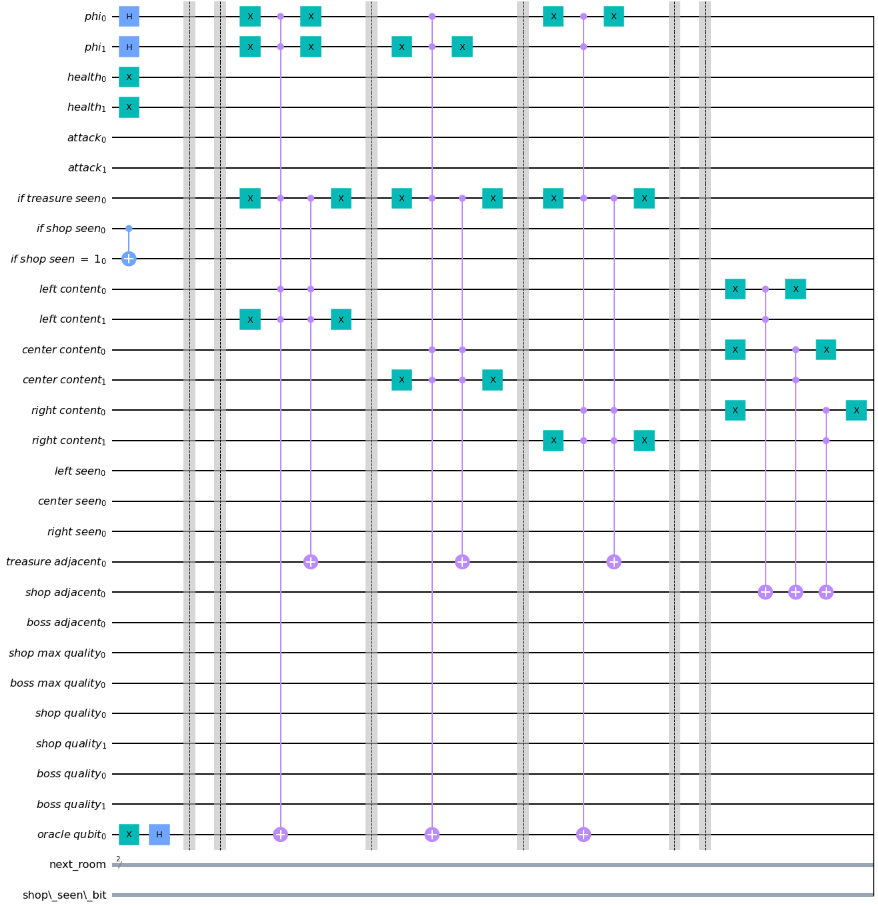
\includegraphics[width=16cm]{immagini_circuito_8_stanze/mega_circ_1.png}
\end{center}
\end{figure}

\begin{figure}[H]
\begin{center}
    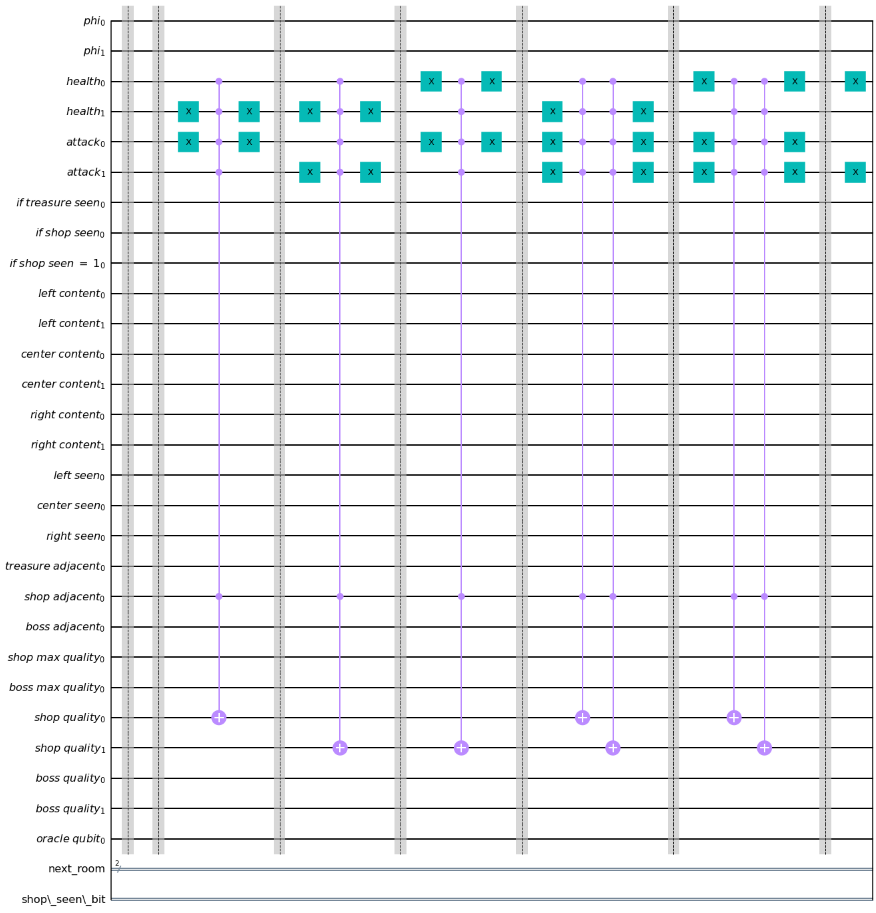
\includegraphics[width=16cm]{immagini_circuito_8_stanze/mega_circ_2.png}
\end{center}
\end{figure}

\begin{figure}[H]
\begin{center}
    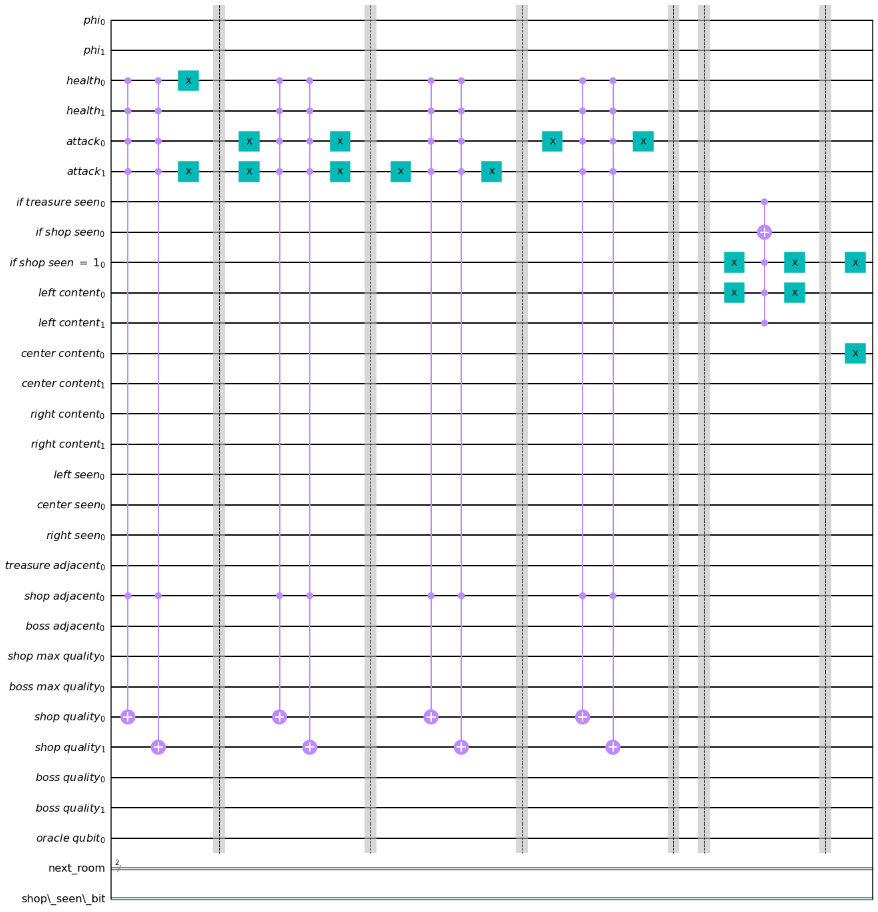
\includegraphics[width=16cm]{immagini_circuito_8_stanze/mega_circ_3.png}
\end{center}
\end{figure}

\begin{figure}[H]
\begin{center}
    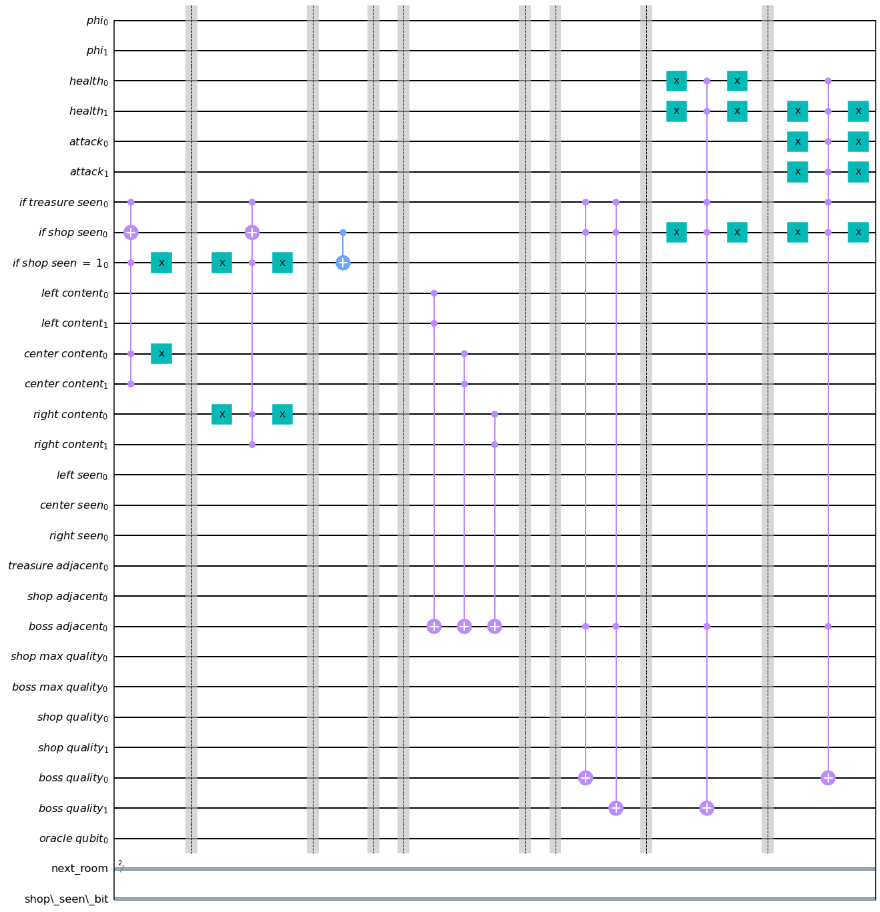
\includegraphics[width=16cm]{immagini_circuito_8_stanze/mega_circ_4.png}
\end{center}
\end{figure}

\begin{figure}[H]
\begin{center}
    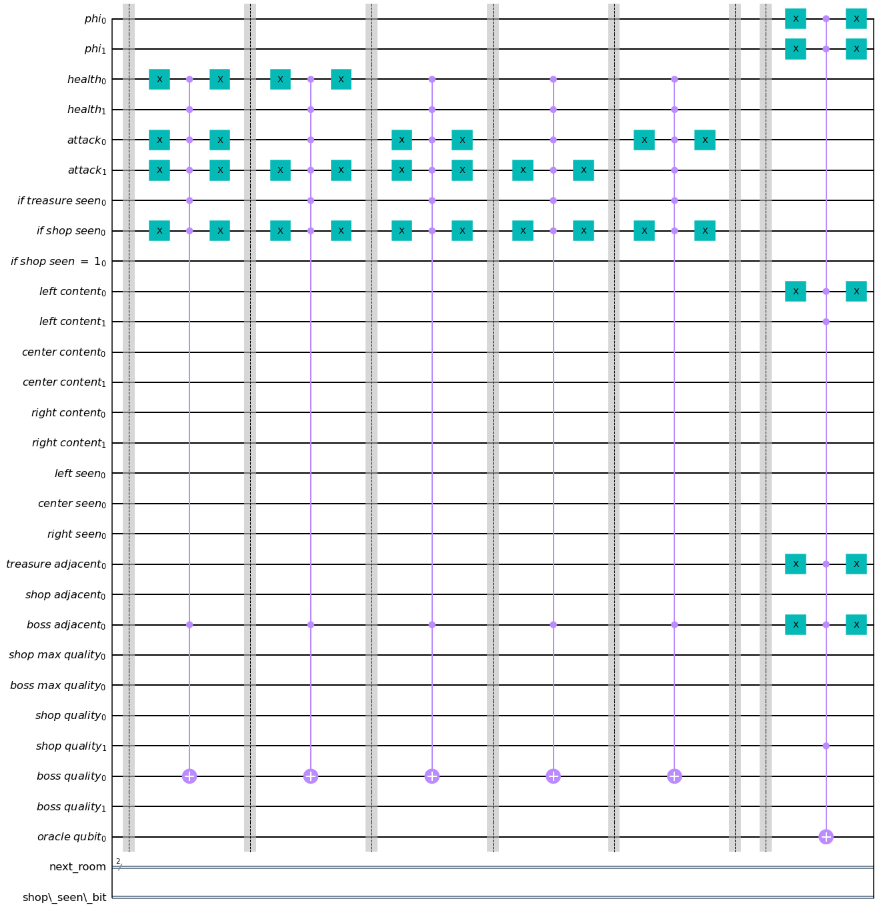
\includegraphics[width=16cm]{immagini_circuito_8_stanze/mega_circ_5.png}
\end{center}
\end{figure}

\begin{figure}[H]
\begin{center}
    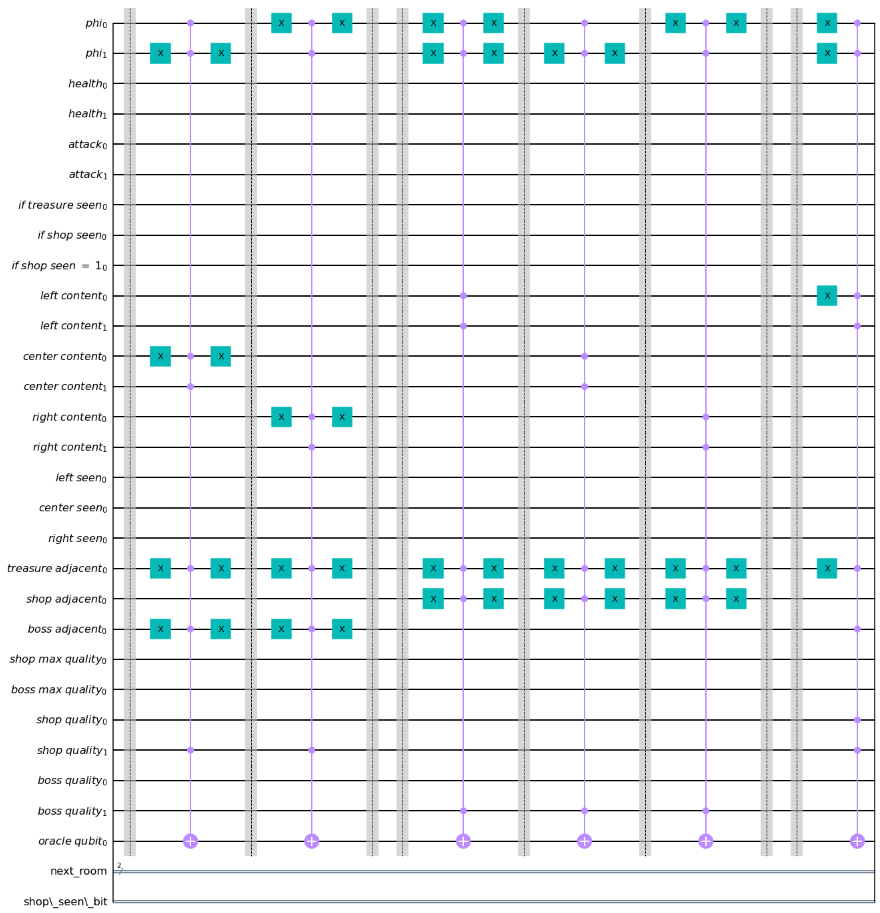
\includegraphics[width=16cm]{immagini_circuito_8_stanze/mega_circ_6.png}
\end{center}
\end{figure}

\begin{figure}[H]
\begin{center}
    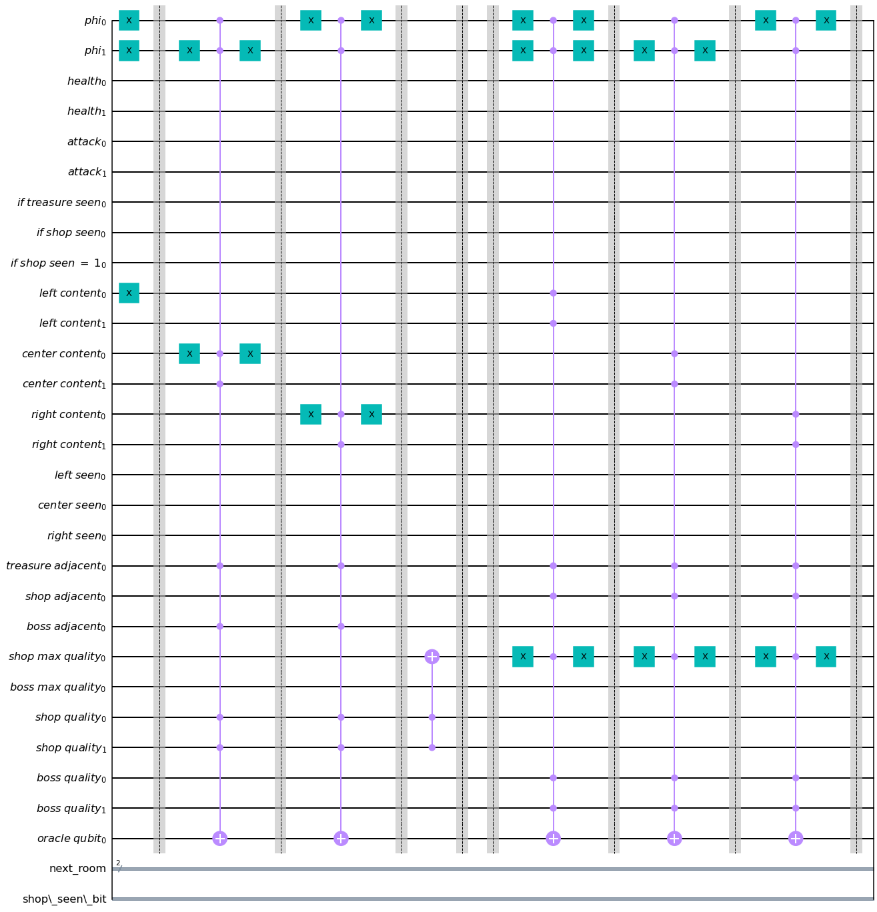
\includegraphics[width=16cm]{immagini_circuito_8_stanze/mega_circ_7.png}
\end{center}
\end{figure}

\begin{figure}[H]
\begin{center}
    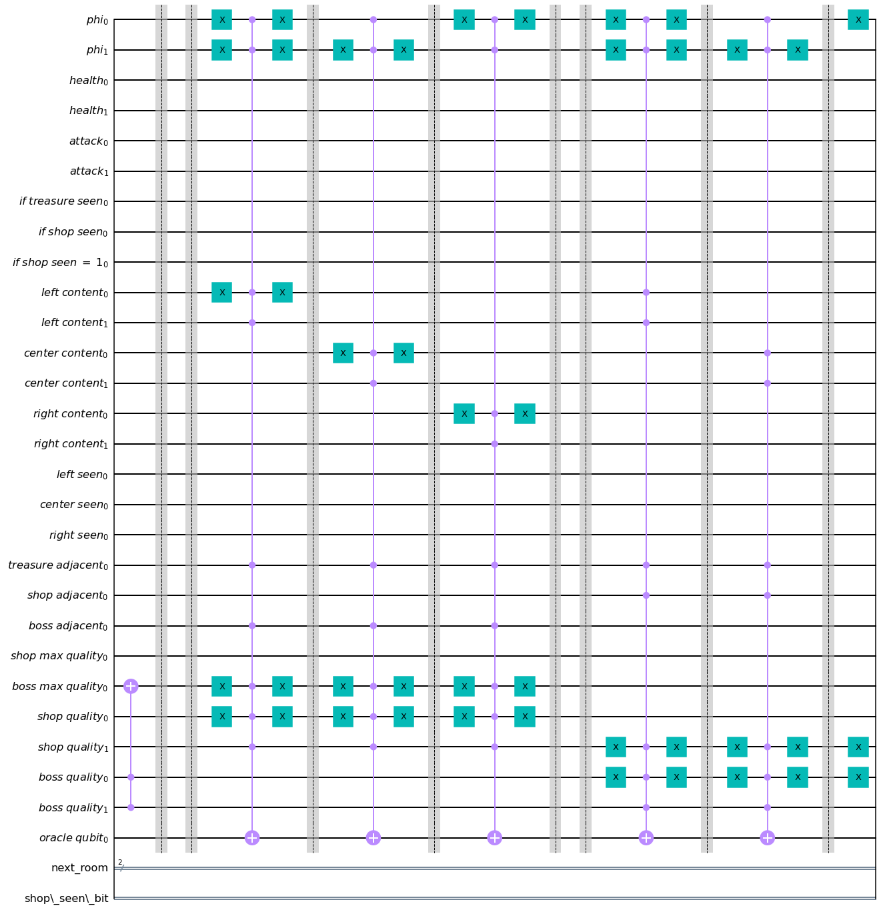
\includegraphics[width=16cm]{immagini_circuito_8_stanze/mega_circ_8.png}
\end{center}
\end{figure}

\begin{figure}[H]
\begin{center}
    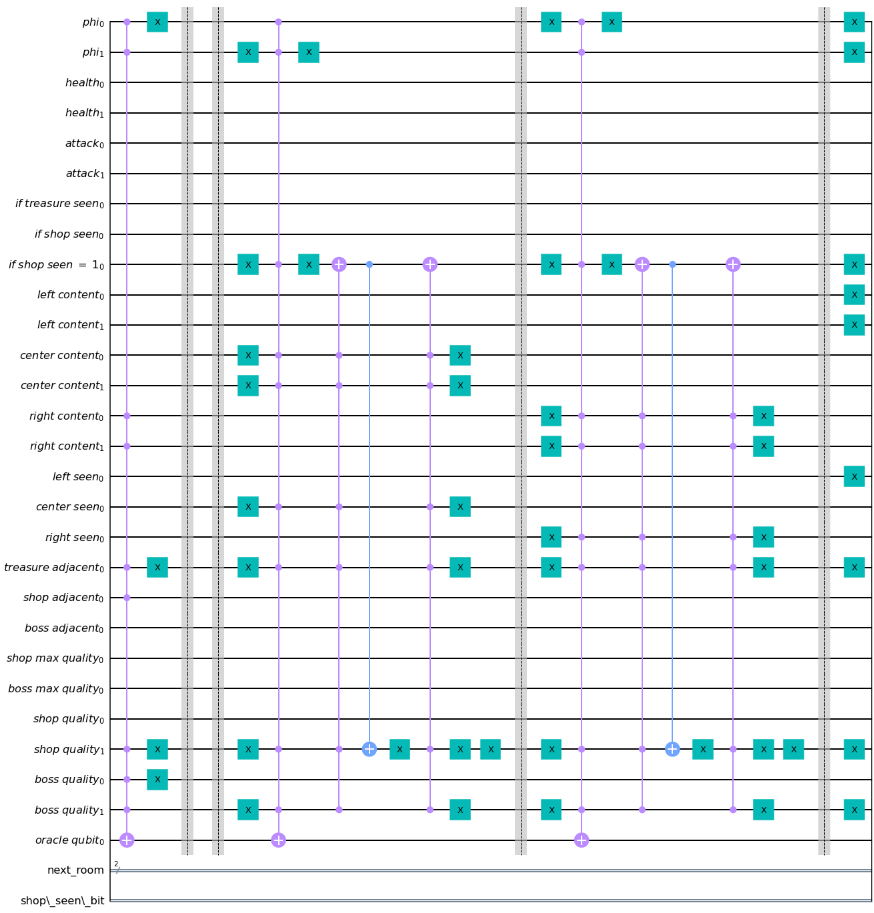
\includegraphics[width=16cm]{immagini_circuito_8_stanze/mega_circ_9.png}
\end{center}
\end{figure}

\begin{figure}[H]
\begin{center}
    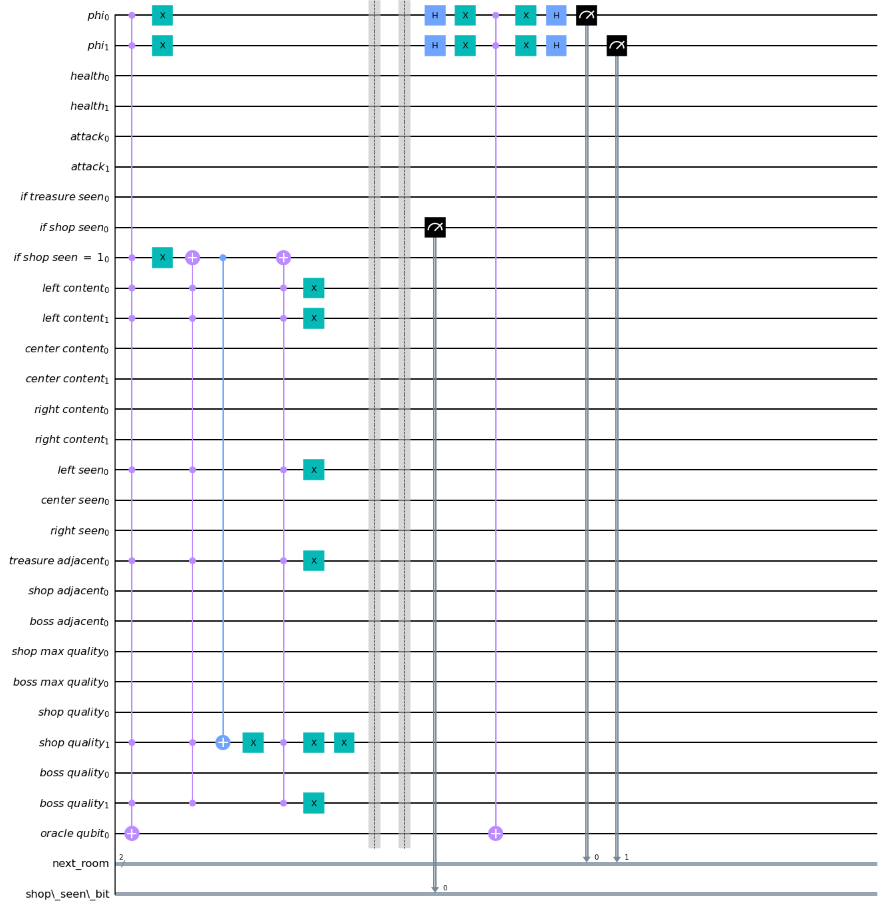
\includegraphics[width=16cm]{immagini_circuito_8_stanze/mega_circ_10.png}
\end{center}
\end{figure}


\bibliographystyle{plain} % We choose the "plain" reference style
%\bibliography{refs}

%\bibliographystyle{ieeetr}
\bibliography{my_bibliography} 



\end{document}

